%%%%%%%%%%%%%%%%%%%%%%%%%%%%%%%%%%%%%%%%%
% Stylish Article
% LaTeX Template
% Version 2.1 (1/10/15)
%
% This template has been downloaded from:
% http://www.LaTeXTemplates.com
%
% Original author:
% Mathias Legrand (legrand.mathias@gmail.com) 
% With extensive modifications by:
% Vel (vel@latextemplates.com)
%
% License:
% CC BY-NC-SA 3.0 (http://creativecommons.org/licenses/by-nc-sa/3.0/)
%
%%%%%%%%%%%%%%%%%%%%%%%%%%%%%%%%%%%%%%%%%

%----------------------------------------------------------------------------------------
%	PACKAGES AND OTHER DOCUMENT CONFIGURATIONS
%----------------------------------------------------------------------------------------

\documentclass[fleqn,10pt]{SelfArx} % Document font size and equations flushed left


\usepackage[english]{babel} % Specify a different language here - english by default

% \usepackage{lipsum} % Required to insert dummy text. To be removed otherwise

\usepackage{xspace}
\usepackage[flushleft]{threeparttable}
\usepackage[nomessages]{fp}% http://ctan.org/pkg/fp
\usepackage{tabu}
\usepackage{appendix}
\usepackage{titlesec}
\usepackage{apptools}
\usepackage{tikz}
%----------------------------------------------------------------------------------------
%	MACROS
%----------------------------------------------------------------------------------------

% !TEX root = ./tech-specification.tex

%  Notations

\newcommand{\B}{\ensuremath{\mathbb{B}}}
\newcommand{\Byte}{\ensuremath{\mathbb{BY}}}
\newcommand{\N}{\ensuremath{\mathbb{N}}}
\newcommand{\emptystring}{\ensuremath{\mathbb{\varepsilon}}}


\newcommand{\st}{\ensuremath{\mathbf{\sigma}}}
\newcommand{\mst}{\ensuremath{\mathbf{\mu}}}
\newcommand{\popstack}{\ensuremath{\mathbf{\delta}}}
\newcommand{\pushstack}{\ensuremath{\mathbf{\rho}}}
\newcommand{\poprstack}{\ensuremath{\mathbf{\delta}^*}}
\newcommand{\pushrstack}{\ensuremath{\mathbf{\rho}^*}}

\newcommand{\transition}{\ensuremath{\mathcal{C}}}
\newcommand{\cost}{\ensuremath{\mathsf{C}}}

\newcommand{\creation}{\ensuremath{\mathrm{\Lambda}}}
\newcommand{\execute}{\ensuremath{\mathrm{\Xi}}}
\newcommand{\execution}{\ensuremath{\mathrm{\Theta}}}
\newcommand{\sstore}{\ensuremath{\mathrm{\Phi}}}

\newcommand{\account}{\ensuremath{\mathbf{\alpha}}}
\newcommand{\contract}{\ensuremath{\mathbf{C}}}


\newcommand{\rec}{\ensuremath{\mathbf{R}}}

\newcommand{\name}{Conflux\xspace}
\newcommand{\tg}{\text{Tree-Graph}\xspace}
% \newcommand{\phvname}[1]{{\fontfamily{phv}\selectfont #1}}
\newcommand{\phvname}[1]{\textsf{#1}}
\newcommand{\op}[1]{\ensuremath{\mathsf{#1}}}

\newcommand{\tx}{\textsf{T}}
\newcommand{\txs}{\textsf{Ts}}
\newcommand{\block}{\textsf{B}}
\newcommand{\gblock}{\textsf{G}}
\newcommand{\ablock}{\textsf{A}}
\newcommand{\genesisblock}{\phvname{Genesis}}
\newcommand{\ommers}{\textsf{U}}
\newcommand{\referees}{\textsf{U}}
\newcommand{\head}{\textsf{H}}
\newcommand{\epoch}{\ensuremath{\textsc{Epoch}}}

\newcommand{\graph}{\textbf{G}}


\newcommand{\reward}{\ensuremath{\textsf{R}}}
\newcommand{\award}{\ensuremath{\textsf{R}_{block}}}
\newcommand{\baseaward}{\ensuremath{\textsf{R}_{base}}}

\newcommand{\feeaward}{\ensuremath{\textsf{R}_{fee}}}
\newcommand{\storageaward}{\ensuremath{\textsf{R}_{storage}}}

\newcommand{\anticone}{\ensuremath{\mathcal{A}}}
\newcommand{\af}{\ensuremath{\mathsf{AF}}}
\newcommand{\basef}{\ensuremath{\mathsf{BF}}}
\newcommand{\wf}{\ensuremath{\mathsf{WF}}}


%% System constants
%	account types
\newcommand{\typenormal}{\ensuremath{[0001]_2}}
\newcommand{\typecontract}{\ensuremath{[1000]_2}}
\newcommand{\typereserved}{\ensuremath{[0000]_2}}

% A new name of {\name} VM
\newcommand{\cvm}{{\textsf EVM}\xspace}


% Unit of {\name} tokens
\newcommand{\unit}{{\sf Drip}\xspace}
\newcommand{\gunit}{{\sf GDrip}\xspace}
\newcommand{\coin}{{\sf Conflux}\xspace}
\newcommand{\coinsign}{{\sf CFX}\xspace}
\newcommand{\ucoinsign}{{\sf uCFX}\xspace}
\newcommand{\cfx}{\coinsign}



% Mathematical notations

\newcommand{\set}[1]{{\left \{{#1} \right \}}}
\newcommand{\ceil}[1]{ {\left\lceil{#1} \right\rceil}}
\newcommand{\floor}[1]{ {\left \lfloor{#1} \right \rfloor}}
\newcommand{\zo}{\ensuremath{ \{ 0, 1 \} }}
\newcommand{\eps}{\ensuremath{\varepsilon}}
\newcommand{\union}{\ensuremath{\cup}}
\renewcommand{\vec}[1]{\ensuremath{\mathbf{#1}}}

\newcommand{\eqdef}{\ensuremath{\equiv}}
% \newcommand{\eqdef}{\ensuremath{:=}}

\newcommand{\true}{\mathsf{True}}
\newcommand{\false}{\mathsf{False}}

% Important functions
\newcommand{\kec}{\ensuremath{\mathsf{KEC}}}
\newcommand{\trie}{\ensuremath{\mathsf{TRIE}}}
\newcommand{\hash}{\ensuremath{\mathsf{Hash}}}
\newcommand{\rlp}{\ensuremath{\mathsf{RLP}\xspace}}
\newcommand{\past}{\ensuremath{\mathsf{PAST}}}
\newcommand{\future}{\ensuremath{\mathsf{FUTURE}}}
\newcommand{\chain}{\ensuremath{\mathsf{CHAIN}}}
\newcommand{\sible}{\ensuremath{\mathsf{SIBLING}}}
\newcommand{\weight}{\ensuremath{\mathsf{Weight}}}
\newcommand{\tolist}{\ensuremath{\mathsf{ToList}}}


\newcommand{\timerchain}{\ensuremath{\mathsf{TimerChain}}}
\newcommand{\timerdis}{\ensuremath{\mathsf{TimerDis}}}

\newcommand{\blockno}{\ensuremath{\mathsf{BlockNo}}}


\newcommand{\risk}{\ensuremath{\mathsf{Risk}}}


\newcommand{\parentf}{\ensuremath{\mathsf{P}}}
\newcommand{\pivotf}{\ensuremath{\mathsf{PIVOT}}}
\newcommand{\parent}[1]{\ensuremath{\mathsf{P}{\left({#1} \right)}}}
\newcommand{\pivot}[1]{\ensuremath{\mathsf{PIVOT}{\left({#1} \right)}}}

\newcommand{\sender}[1]{\ensuremath{\mathsf{S}{\left({#1} \right)}}}
\newcommand{\receiver}[1]{\ensuremath{\mathsf{S}{\left({#1} \right)}}}

\newcommand{\senderf}{\ensuremath{\mathsf{S} }}
\newcommand{\epf}{\ensuremath{\mathsf{EPOCH} }}


\newcommand{\cfs}{\ensuremath{\mathsf{CFS}}}
\newcommand{\gused}{\ensuremath{\mathsf{Gas_{used}}}}
\newcommand{\sol}[1]{\texttt{\textbf{#1}}}
\newcommand{\solkw}[1]{{\color{blue}{\texttt{#1}}}}



\newcommand{\pow}{\ensuremath{\mathsf{PoW}}}
\newcommand{\mpethash}{\ensuremath{\mathsf{MpEthash}}}

\newcommand{\quality}{\ensuremath{\mathsf{QUALITY}}}
\newcommand{\offset}{\ensuremath{\mathsf{OFFSET}}}

\newcommand{\hcancel}[1]{%
	% -{#1}
    \tikz[baseline=(tocancel.base)]{
        \node[inner sep=1pt,outer sep=0pt] (tocancel) {{$#1$}};
        \draw[black] (tocancel.south west) -- (tocancel.north east);
    }%
}%
\newcommand{\compressedmix}{\ensuremath{\mathbf{m}_{\mathrm{c}}}}
\newcommand{\mpmix}{\ensuremath{{m}_{\mathrm{p}}}}

\newcommand{\seedhash}{\ensuremath{\vec{s}_{\mathrm{h}}}}
\newcommand{\dataset}{\ensuremath{\vec{d}}}
\newcommand{\headernon}{\ensuremath{\head_{\hcancel{n}}}}


%%%%%%%%%%%%%%%%%%%%%%%%
% Setting of parameters
%%%%%%%%%%%%%%%%%%%%%%%%

\newcommand{\chainid}{2}
% \newcommand{\chainid}{{\color{red} Conflux Chain ID}}

\newcommand{\txepochbound}{{\color{red}100000}}

\newcommand{\startblockgastlimit}{3\times 10^7}
\newcommand{\collateralperbyte}{\frac{10^{18}}{1024}}
\newcommand{\collateralperbyteline}{10^{18}/{1024}}
\newcommand{\startblockgastlimitline}{30000000}
\newcommand{\maxblocksize}{{$200$} KB}
\newcommand{\maxblocksizeinbytes}{\ensuremath{204800}}
\newcommand{\snapshotperiod}{100000}
\newcommand{\minblockgaslimit}{10^7}


%%%%%%%%%%%%%%%%%%%%
% Internal Contracts
%%%%%%%%%%%%%%%%%%%%%%%%
\newcommand{\admincontract}{{\sf 0x0888000000000000000000000000000000000000}}
\newcommand{\sponsorcontract}{{\sf 0x0888000000000000000000000000000000000001}}
\newcommand{\stakingcontract}{{\sf 0x0888000000000000000000000000000000000002}}

%%%%%%%%%%%%%%%%%%%%
% Mining Schedule
%%%%%%%%%%%%%%%%%%%%%%%%
\newcommand{\blocktime}{0.5}
\FPeval{\blocktimeunix}{clip(\blocktime*1000000)}
\FPeval{\blockinyear}{clip(31536000/\blocktime)}

\newcommand{\quarter}{\mathsf{QRT}}
\newcommand{\initialblockreward}{7}
\newcommand{\eventualblockreward}{1.75}


\newcommand{\decayperiodinday}{91.25}
\FPeval{\decayperiodinblock}{clip(\decayperiodinday*86400/\blocktime)}
% \newcommand{\decayperiod}{15768000} % a quarter = 60*60*24*365/4 seconds, times 2 blocks/s

\newcommand{\decaystartinquarter}{16}
\newcommand{\decayendinquarter}{48}
\FPeval{\decayquarters}{clip(\decayendinquarter-\decaystartinquarter)}
\FPeval{\decaystartinyear}{clip(\decaystartinquarter/4)}
\FPeval{\decayyears}{clip(\decayquarters/4)}

\newcommand{\halfendinyear}{10}
% \FPeval{\decayendinblock}{round(\decayperiodinblock*\halfendinyear*365/\decayperiodinday,0)}

\newcommand{\halfinperiod}{16}
\FPeval{\decayfactor}{round((0.5)^(1/\halfinperiod),3)}
\FPeval{\decayby}{round(1-\decayfactor,3)}
\FPeval{\decaybypercent}{round(\decayby*100,1)}
% \newcommand{\decaypercent}{4.2}
% \FPeval{\decayfactor}{round(1-\decaypercent/100,3)}

\newcommand{\genesistotal}{5000000000}
\newcommand{\mininginflationfirstperiod}{0.0356}
% \newcommand{\mininginflationfirstperiod}{0.05}

% \FPeval{\initialblockreward}{round(\genesistotal*\mininginflationfirstperiod/\decayperiodinblock,1)}
% \newcommand{\blockreward}{900}
% \FPeval{\eventualblockreward}{round(\initialblockreward*(\decayfactor^40),2)}

\newcommand{\targetinflationpercent}{2}



\newcommand{\dfb}{5}
\newcommand{\minerfreeze}{12}
\newcommand{\deferblk}{{\dfb}\xspace}
\FPeval{\dfbresult}{clip(\dfb+1)}
\FPeval{\minerfreezeexec}{clip(\dfb+\minerfreeze)}


% !TEX root = ./contract.tex

%% GHAST parameters

\newcommand{\timerweight}{{\color{red}180}}

\newcommand{\heavyw}{\mathrm{h}}
\newcommand{\heavywvalue}{{\color{red}250}}
% \newcommand{\palpha}{\alpha}
% \newcommand{\pbeta}{\beta}
\newcommand{\palpha}{{\color{red}1000}}
\newcommand{\valuepbeta}{240}
\newcommand{\pbeta}{{\color{red}\valuepbeta}}
\FPeval{\pbetam}{clip(\valuepbeta-1)}


\newcommand{\numberofommers}{100}

% Incentive Parameter

\newcommand{\anticonecountepoch}{{10}}
\newcommand{\anticoneconstant}{{100}}

\newcommand{\difficultyadjustperiod}{5000}

\newcommand{\interest}{{4\%}\xspace}
\newcommand{\annualinterest}{{4.08\%}\xspace}


\newcommand{\commissionrate}{{0.0005}}
\FPeval{\commissionpercent}{clip(round(\commissionrate*100,3))}

\newcommand{\commissiondecayinday}{91.25}
\FPeval{\commissiondecayinblock}{clip(\commissiondecayinday*86400/\blocktime)}

%%  Gas limit and difficulty adjustment

\newcommand{\mingas}{{21000}\xspace}
\newcommand{\mingaslimit}{{5000}\xspace}

% \newcommand{\startdifficulty}{5\times 10^9}
% \newcommand{\startdifficultyline}{5000000000}
\newcommand{\startdifficulty}{3\times 10^4}
\newcommand{\startdifficultyline}{30000}

\newcommand{\mindifficulty}{\startdifficultyline\xspace}
\newcommand{\diffup}{{1.5}\xspace}
\newcommand{\diffdown}{{0.5}\xspace}


\newcommand{\eragap}{50000}
\FPeval{\eraexample}{clip(2*\eragap+100)}

%% Storage price
\newcommand{\sunitsize}{{64B}\xspace}
\newcommand{\fsunitprice}{\frac{1}{16}}
\newcommand{\sunitprice}{$1/16$ \coinsign}
\newcommand{\storagepertoken}{{$1$KB}\xspace}
\newcommand{\storagebytepertoken}{1024}



% Version controls
% \newcommand{\newversion}[1]{{\color{blue} #1}}
\newcommand{\newversion}[1]{{#1}}
% \newcommand{\oldversion}[1]{{\color{gray} {#1}}}
\newcommand{\oldversion}[1]{{\color{gray} {}}}


%  Remark and comments

% slience all the notes in the publish version
% \newcommand{\underdiscussion}[1]{}
% \newcommand{\guangsays}[1]{}
% \newcommand{\note}[1]{}
% \newcommand{\todo}[2]{}

\newcommand{\guangsays}[1]{{\color{red}\textbf{}#1}}
\newcommand{\underdiscussion}[1]{{\color{blue}\textbf{}#1}}
\newcommand{\note}[1]{{\color{red} $\langle$NOTE: #1$\rangle$}}
\newcommand{\todo}[2]{{\color{red} $\langle$TODO [#1]: #2$\rangle$}}

%----------------------------------------------------------------------------------------
%	ALGORITHMS
%----------------------------------------------------------------------------------------

\usepackage[figure,vlined,linesnumbered]{algorithm2e}
%----------------------------------------------------------------------------------------
%	STRIKE OUT
%----------------------------------------------------------------------------------------
\usepackage[normalem]{ulem}


%----------------------------------------------------------------------------------------
%	COLUMNS
%----------------------------------------------------------------------------------------

\setlength{\columnsep}{0.55cm} % Distance between the two columns of text
\setlength{\fboxrule}{0.75pt} % Width of the border around the abstract
\usepackage{array,tabularx,multirow}

%----------------------------------------------------------------------------------------
%	COLORS
%----------------------------------------------------------------------------------------

\definecolor{color1}{RGB}{0,0,90} % Color of the article title and sections
\definecolor{color2}{RGB}{150,150,80} % Color of the boxes behind the abstract and headings
\definecolor{color3}{RGB}{120,120,10} % Color of the boxes behind the abstract and headings


\definecolor{backgroundcolor}{RGB}{250,250,233} % Color of the page background

\pagecolor{backgroundcolor}
%----------------------------------------------------------------------------------------
%	HYPERLINKS
%----------------------------------------------------------------------------------------

\usepackage{hyperref} % Required for hyperlinks
\hypersetup{hidelinks,colorlinks,breaklinks=true,urlcolor=color3,citecolor=color1,linkcolor=color1,bookmarksopen=false,pdftitle={Title},pdfauthor={Author}}

\usepackage{cleveref}

\usepackage{tabu} %requires array.

%This should be the last package before \input{Version.tex}
\PassOptionsToPackage{hyphens}{url}\usepackage{hyperref}
% "hyperref loads the url package internally. Use \PassOptionsToPackage{hyphens}{url}\usepackage{hyperref} to pass the option to the url package when it is loaded by hyperref. This avoids any package option clashes." Source: <https://tex.stackexchange.com/questions/3033/forcing-linebreaks-in-url/3034#comment44478_3034>.
% Note also this: "If the \PassOptionsToPackage{hyphens}{url} approach does not work, maybe it's "because you're trying to load the url package with a specific option, but it's being loaded by one of your packages before that with a different set of options. Try loading the url package earlier than the package that requires it. If it's loaded by the document class, try using \RequirePackage[hyphens]{url} before the document class." Source: <https://tex.stackexchange.com/questions/3033/forcing-linebreaks-in-url/3034#comment555944_3034>.
% For more information on using the hyperref package, refer to e.g. https://en.wikibooks.org/w/index.php?title=LaTeX/Hyperlinks&stable=0#Hyperlink_and_Hypertarget.

\makeatletter
 \newcommand{\linkdest}[1]{\Hy@raisedlink{\hypertarget{#1}{}}}
\makeatother
\usepackage{seqsplit}



%----------------------------------------------------------------------------------------
%	ARTICLE INFORMATION
%----------------------------------------------------------------------------------------
\IfFileExists{version.tex}{
    \input{version}
}{
    \newcommand{\fdate}{\today}
    \newcommand{\version}{Temporary}
}

\JournalInfo{[Octopus v1.0.0]} % Journal information
\Archive{Spec Version: \version\\\fdate} % Additional notes (e.g. copyright, DOI, review/research article)

\PaperTitle{{\name} Protocol Specification} % Article title

\Authors{Chenxing Li\textsuperscript{$\dagger$}, Guang Yang\textsuperscript{$\dagger$} } % Authors
\affiliation{\textsuperscript{$\dagger$}\textit{{\name} Dev Team} 
\begin{figure}[ht]\centering

\includegraphics[width=0.5\linewidth]{figs/logo}
\end{figure}
} % Author affiliation
%\affiliation{\textsuperscript{2}\textit{Department of Chemistry, University of Examples, London, United Kingdom}} % Author affiliation
%\affiliation{*\textbf{Corresponding author}: john@smith.com} % Corresponding author

\Keywords{} % Keywords - if you don't want any simply remove all the text between the curly brackets
\newcommand{\keywordname}{Keywords} % Defines the keywords heading name

%----------------------------------------------------------------------------------------
%	ABSTRACT
%----------------------------------------------------------------------------------------

\Abstract{
The success of Bitcoin and its follow-ups have demonstrated the value of decentralized consensus system among anonymous participants not trusting each other.
On top of the consensus network there can be a public ledger or even a general state transition machine, 
such that all participants agree on the state of the ledger or the state machine.
Conceptually the state machine can be Turing-complete and hence essentially a ``world computer'' shared by all participants, whose results cannot be tampered by any single person or entity.
However, the processing power of the shared state machine is currently bottlenecked on the throughput of underlying consensus system.

{\name} implements a Turing-complete state machine on top of a high-throughput consensus network.
% , which is capable of handling thousands of transactions per second.
To achieve a throughput of thousands of transactions per second, {\name} guarantees consensus on the total order of blocks organized in a \tg.
In this way, all forked blocks contribute to the security and throughput of {\name} as well.
In this work we discuss {\name} protocol design and implementation specifications.
}

%----------------------------------------------------------------------------------------

\begin{document}

\flushbottom % Makes all text pages the same height

\maketitle % Print the title and abstract box

\setcounter{tocdepth}{3}

\tableofcontents % Print the contents section

\thispagestyle{empty} % Removes page numbering from the first page

%----------------------------------------------------------------------------------------
%	ARTICLE CONTENTS
%----------------------------------------------------------------------------------------
\newpage
%------------------------------------------------
%%%%%%%%%%%%%%%%%%%%%%%%%%%%%%%%%%%%%%%%
% \section{Introduction}
% !TEX root = ./tech-specification.tex

%%%%%%%%%%%%%%%%%%%%%%%%%%%%%%%%%%%%%%%%

\section{Introduction}

%\addcontentsline{toc}{section}{Introduction} % Adds this section to the table of contents

Since the born of Bitcoin, various blockchain projects have demonstrated extraordinary success with the power of consensus among permissionless and trustless parties.
The most successful blockchain project after Bitcoin is widely considered to be Ethereum, which generalizes the blockchain paradigm from a specialized value-transfer system to a more generalized Turing-complete state machine that allows conceptually all kinds of computation.
This generalized state machine, known as \emph{Ethereum Virtual Machine} (EVM), makes the Ethereum network essentially a decentralized computing platform 
where the state advances on input of transactions.
Sometimes Ethereum is referred to as the ``world computer'' that nobody can shut down, 
except that its processing power is rather poor and severely bounded by the throughput of underlying consensus.

The consensus throughput of Bitcoin is (in expectation) one block per $10$ minutes, with block size $1$MB (or $2$MB with Segregated Witness (segwit)).
Bitcoin is set to small block size and low generation rate mainly for security concerns.
Intuitively, when there is no adversary, the natural probability of forks is proportional to the ratio of  block broadcasting time to block (generation) time,
since under the longest chain rule honest mining power may keep working on a fork during the propagation of a newly mined block.
Ethereum applies a tailored version of GHOST rule \cite{GHOST} and smaller block size to achieve a much shorter block time, i.e. roughly $<100$KB per $15$ seconds.
Inclusive Block Chain Protocol \cite{Inclusive} is a ``block-DAG'' proposal which defines a total order of blocks in a directed acyclic graph (DAG) rather than a chain, with the major advantage over GHOST that all forked blocks contribute to the consensus throughput as well. 
Another line of scaling techniques trades security and decentralization for scalability by using sharding, sidechains, or other second layer extensions.
In extreme cases, centralized and somehow permissioned consensus systems are implemented in practice.


{\name} is a project which aims at building a high throughput first layer consensus system without any compromises in security and decentralization; a generalized computation platform that securely processes at least thousands of transactions per second which makes the  throughput of consensus is no more a bottleneck.
The positioning of {\name} is a strong backbone consensus network on which a numerous number of unprecedented applications and extensions can germinate and thrive.
Technically, we follow a similar idea as \cite{Inclusive} but organize blocks in a \tg, 
which enables a fast implementation of the {\name} protocol.


%------------------------------------------------
%%%%%%%%%%%%%%%%%%%%%%%%%%%%%%%%%%%%%%%%
% \section{Conventions}
% !TEX root = ./tech-specification.tex

%%%%%%%%%%%%%%%%%%%%%%%%%%%%%%%%%%%%%%%%
\section{Conventions}

Throughout this document, we use the following conventional notations:  
\begin{itemize}[nosep]
	\item $\B$ denotes the set of bit values, i.e. $\B\eqdef \zo$. 
	$\Byte$ denotes the set of byte values, i.e. $\Byte\eqdef \set{0,\dots,255}$.

	\item $\N$ denotes the set of non-negative integers. 


	\item For every $n\in \N$, we use $\B_n$ to denote a binary string of $n$ bits, and $\Byte_n$ for a string of $n$ bytes. In particular, $\Byte=\B_8$.
	
	\begin{itemize}
		\item Furthermore, we denote by $\B^*$ and $\Byte^*$ the set of binary or byte strings of arbitrary length, i.e. $\B^*\eqdef \cup_{i\in\N} \B_i$ and $\Byte^*\eqdef \cup_{i\in\N} \Byte_i$. 
	
		\item For convenience, we let $\N_{n}\eqdef\set{0,1,\dots, 2^n-1}$  be the set of non-negative integers smaller than $2^n$.

		\item The empty string (or the empty series) is denoted by $\emptystring$, which is distinguished from the empty set denoted by $\varnothing$.
	\end{itemize}

	\item Numbers are in decimal base by default. Binary numbers are indicated with square brackets with subscripts, e.g. $[0100]_2$ is the $4$-bit binary representation of $4$. The subscript \textsf{ch} represents the character representation of bit string, e.g. $[{\sf ab}]_{\sf ch}=[6162]_{16}=[0110000101100010]_2$.

	\item When interpreting 256-bit binary values from $\N_{256}$ as integers, the representation is big-endian.

	\item When a 256-bit machine datum in $\B_{256}$ is converted to and from a 160-bit address or hash in $\B_{160}$, the rightwards (low-order for BE) 160 bits (20 bytes) are used and the leftmost 96 bits (12 bytes) are discarded or filled with zeros, thus the integer values (when the bytes are interpreted as big-endian) are equivalent.

	\item Tuples are typically denoted with bold upper case letters such as $\mathbf{A}$. 
	For frequently used tuples, we denote by $\tx$ for a {\name} transaction, $\block$ for a {\name} block, and $\head$ for the header of a block. 
	\begin{itemize}[nosep]
		\item Subscripts can be added to refer to an individual component in the tuple, e.g. $\tx_n$ denotes the nonce of the transaction $\tx$.
		The type of referred components is the same as the type of subscript, e.g. $\block_{\head}$ denotes the header of a block $\block$, where the header itself is another tuple of elements. 
		For succinctness we also write $\head(\block)\eqdef \block_{\head}$ and sometimes simply $\head$ when there is no ambiguity.
		\newversion{
			Also for succinctness, we sometimes use $\block$ and $\head$ interchangeably if there is no ambiguity, e.g. $\block_d$ stands for the target difficulty of block $\block$, which is formally denoted as $\head(\block)_d$ or $\block_{\head_d}$.
		}

		\item In case we are considering many transactions or blocks, we add superscripts to refer to a specific one of them, e.g. $\tx^1$ denotes the first transaction in a sequence.
	\end{itemize}

	\item \newversion{The \tg structure of blocks is typically denoted by $\graph$, which is a graph consisting of blocks represented by vertices and parent/referee relations represented by two kinds of directed edges.}	   

	\item Scalars and fixed-length sequences of elements (arrays, strings, and vectors) are denoted with normal lower case letters, e.g. $n$ is used to denote a transaction nonce. 
	Those with a special meaning may be denoted with Greek letters.

	\item Sequences of potentially arbitrary number of elements are typically denoted with bold lower case letters, e.g. $\mathbf{o}$ is used to denote the byte sequence generated as the output data of a message call.

	\item The highly structured state values are typically denoted with bold lower case Greek letters, e.g. $\st$ (and its variants) is used to denote the world-state, and $\mst$ for machine state.
	% \begin{itemize}[nosep]
		
	% \end{itemize}

	\item Square brackets are used to index subsequences of a sequence, with index starting from $0$, e.g. $\mst_{\mathbf{s}}[0]$ refers to the first item on the machine's stack and $\mst_{\mathbf{m}}[0\dots 31]$ denotes the first $32$ items of the machine's memory.
	\begin{itemize}[nosep]
		\item Some objects like the global state $\st$ is interpreted as a set of key/value pairs.
		Thus the square bracket after $\st$ refers to corresponding value of the given key (i.e., account address). 
		\item Square brackets use negative index to access an array from the end like Python, e.g. $\mst_{\mathbf{s}}[-1]$ refers the last item on the machine's stack. 
	\end{itemize}


	\item Functions are typically denoted by upper case letters and subscripts are used for specialized variants, e.g. $C$ is the general cost function and $C_{\op{CALL}}$ is the cost function for the $\op{CALL}$ operation.
	Specific functions operating on states are denoted by upper case calligraphic letters, e.g. $\transition$ denotes the {\name} global state transition function.
	\begin{itemize}[nosep]
		\item For every function $F$ defined on $D$, we let $F^*$ denote the function on range $D^*$ that element-wise applies $F$ on its input items, i.e. $F^*\big( \left(x_1, x_2, \dots\right) \big) \eqdef \left( F(x_1), F(x_2),\dots \right)$. 
	\end{itemize}

	\item The superscript of a function with parentheses like $f^{(i)}$ represents call function $f$ for $i$ times recursively. Formally, $f^{(1)}(\cdot)\eqdef f(\cdot)$ and $f^{(i)}(\cdot)\eqdef f^{(i-1)}(f(\cdot))$ for $i\ge 2$.
	
	\item The indicator function $\mathbb{I}(\cdot)$ converts a boolean variable to integer. Formally, $\mathbb{I}(\true)=1$ and $\mathbb{I}(\false)=0$.

\end{itemize}  

\smallskip

Frequently used functions:
\begin{itemize}[nosep]
	\item $\parentf$: the \emph{parent function}  takes a block $\block$ as input and returns the parent block $\block'$, i.e. $\block'$ is referenced in $\block$ and designated as the parent of $\block$.
	Formally, $\parentf(\block)\eqdef \block':\kec\left(\rlp(\block')\right)=\head(\block)_{p}$.\footnote{One may argue whether $\parentf$ is well-defined since $\kec$ has collisions. However, as long as the collision cannot be found in practical situations, the function $\parentf$ only need to look up such a $\block'$ from existing blocks and returns $\bot$ if there is none.}

	\item $\chain$: the \emph{chain function} takes a block $\block$ as input and returns the chain from genesis block to block $\block$ following only parent edges. Formally, for genesis block $\gblock$, $\chain(\gblock)\eqdef\gblock$; For other blocks $\block$, $\chain(\block)\eqdef\chain(\parentf(\block))\circ \block$.
	
	\item $\sible$: the \emph{sibling function} takes a block $\block$ as input and returns the blocks which have the same parent as $\block$. Formally, $\sible(\block)\eqdef\{\block' \;|\; \parentf(\block')=\parentf(\block) \wedge \block'\neq \block\}$.

	\item $\past$: the \emph{past function}  takes a block $\block$ as input and outputs all blocks in the ``past set of $\block$'', i.e. all blocks that are directly or indirectly referenced by $\block$.
	The set $\past(\block)$ does not include $\block$, since $\block$ cannot reference itself.
	
	\item $\future$: the \emph{future function} takes a \tg $\graph$ and a block $\block\in\graph$ as inputs and outputs all blocks in the  ``future set of $\block$''. Formally, $\future(\block;\graph)\eqdef\{\block' \in \graph \mid \block \in \past(\block')\}$. 

	\item $\epf$: the \emph{epoch function} takes a block $\block$ as input and returns a sequence of all blocks in the epoch of $\block$, sorted as in the \name total order defined in Section~\ref{sec:total order}.


	\item \newversion{
		\linkdest{blockno}{$\blockno$}: the \emph{block number function} takes a \tg $\graph$ and a block $\block$ as inputs and returns the index of $\block$ in the total order of blocks specified by $\graph$, where the index starts from $0$.
		In particular, for the genesis block $\gblock$ and for every \tg $\graph$ there must be $\blockno(\gblock;\graph)=0$.
		Note that $\blockno(\block;\graph)$ depends on $\graph$ and it is different from $\past(\block)$ which is fully determined by $\block$.
		For every $\graph$ and $\block\in\graph$ there must be $\blockno(\block;\graph)\ge \past(\block)$ since all blocks in $\past(\block)$ precede $\block$ in the total order.
		Furthermore, for $\block,\block'\in\graph$ and $\block\ne\block'$, there must be $\blockno(\block;\graph)\ne\blockno(\block';\graph)$ because distinct blocks cannot have identical index in the total order.
		When the \tg $\graph$ is clear from context, we may write $\blockno(\block)$ for succinctness.
	}


	\item $\pivotf$: the \emph{pivot function} takes a block $\block$ as input and outputs the pivot block in the epoch of $\block$.

	\item $\senderf$: the \emph{sender function} takes a transaction $\tx$ as input and returns the sender of $\tx$, where in particular the sender is represented by its address. 

	\item \linkdest{rlp}{$\rlp$}: this is the serialization function that encodes an input of arbitrary length into a structured binary data, i.e. a byte array explicitly containing information about the length of the input.
	For more details see Appendix B in \cite{ETH_yellow}.

	\item $\tolist$: this function takes a key/value set whose keys are integers or bit/byte sequences the values are integers. It outputs a sequence of key/value pairs for the entry with non-zero value in ascending order or lexicographical order of key.


	\item $\trie$: the trie function maps an arbitrary-length binary byte array $\mathbf{s}$ into a  $256$-bit commitment that represents the database storing $\mathbf{s}$ in a modified Merkle Patricia tree (trie). 

	\item $\kec$: the Keccak $256$-bit cryptographic (collision-resistant) hash function that maps an arbitrary-length binary byte array to a random-looking binary string in $\B_{256}$.
	Furthermore, we assume $\kec$ implements a \emph{random oracle}, i.e. finding a random collision of $\kec$ requires in expectation roughly $2^{128}$ attempts and a specific collision requires $2^{256}$.
	Similarly, $\kec512$ refers to the $512$-bit cryptographic hash function Keccak-512.

	\item $\pow$: this is the proof-of-work function, which takes a block header as input and returns a scalar in $\B_{256}$.
	

	\item \newversion{$\quality$: this is a measurement of the  proof-of-work quality of a given block,
	i.e. how unlikely it is to find such a block. 
	It takes a block or a block header as input and outputs a scalar in $\N_{256}$. 
	Essentially, a block $\block$ with header $\head=\head(\block)$ has quality 
 	$\quality(\block)\eqdef 
 	\quality(\head)\eqdef 
 	\left\lfloor 2^{256}/\left(\pow(\head) - \left[\head_n[1\dots127]\right]_2\times 2^{128} +1\right) \right\rfloor$ except for a few marginal cases.
 	See Section~\ref{subsec:quality} for more details.}
\end{itemize}


\subsection{Value}
To incentivize the maintenance of the {\name} network and charge users for consumption of resources,
{\name} has an intrinsic currency called {Conflux Coin} or simply \coin, denoted by \coinsign for short.
The smallest subdenomination is denoted by \unit,
in which all values processed in \name are integers.
One \coin is defined as $10^{18}$ \unit.
Frequently used subdenominations of {\name} are list as follows:
\par
\begin{center}
\begin{tabular}{cl}
\toprule
Multiplier (in \unit) & Name \\
\midrule
$10^{0~}$ & \unit \\
% $10^{6}$ & TBD \\
$10^{9~}$ & \gunit \\
$10^{12}$ & \ucoinsign \\
% $10^{15}$ & TBD \\
$10^{18}$ & \coin (\coinsign) \\
\bottomrule
\end{tabular}
\end{center}










%------------------------------------------------

%%%%%%%%%%%%%%%%%%%%%%%%%%%%%%%%%%%%%%%%
% \section{Basic Components}
% !TEX root = ./tech-specification.tex

%%%%%%%%%%%%%%%%%%%%%%%%%%%%%%%%%%%%%%%%
%------------------------------------------------

\section{Basic Components}
In an overview, the {\name} world-state consists of a list of accounts and the associated account states, and the global state is updated via transactions. 
The {\name} blockchain stores all processed transactions in blocks, together with necessary information in block headers which enables a total ordering of all blocks.
In this section we discuss the meaning of accounts, transactions and blocks in more details.


\subsection{Accounts}
\label{subsec:accounts}

The {\name} global state is described in an account model, with the basic storage component called an \emph{account}.
Every actor, which is either a person or an entity that is able to interact with the {\name} world, has its necessary information stored in an account $\account$  as a key/value pair $(\account_{addr}, \account_{state})$ of address and corresponding states. 
The account address $\account_{addr}$ is a 160-bit identifier. The account state $\account_{state}= (\account_{basic},\account_{code}, \account_{storage},\account_{deposit},\account_{vote})$ consists of five components. The account basic state $\account_{state}$, the code info $\account_{code}$, the deposit list $\account_{deposit}$ and the vote list $\account_{vote}$ are four serialized sequences in an $\rlp$ structure (c.f. \cite{ETH_yellow}). The account storage $\account_{storage}$ is a set of key-value pairs which map 256-bit address to a serialized storage information in an $\rlp$ structure. 
Furthermore we note that each account $\account$ is associated with a pair of public key and private key $\left(\account_{pubkey}, \account_{prikey}\right)$.
The account address is the concatenation of $4$-bit type indicator and a $156$-bit digest of the associated public key: 
\begin{equation}\label{eq:account-address}
	\account_{addr} \eqdef \mathsf{Type}_{\account} \circ \kec \left( \account_{pubkey} \right)[100\dots 255]
\end{equation}
where $\mathsf{Type}_{\account}\in \B_4$ is the type indicator,
which is $\mathsf{Type}_{\account}=\typenormal$ for \emph{normal accounts} (a.k.a. \emph{non-contract accounts}), $\mathsf{Type}_{\account}=\typecontract$ for \emph{(Solidity) contracts},
and $\mathsf{Type}_{\account}=\typereserved$ for \emph{built-in/reserved contracts} (a.k.a. \emph{``precompiled contracts''}).


For succinctness and convenience, and as long as there is no ambiguity, we will write $\account$ without subscript for the state of an account and let $a\eqdef \account_{addr}$ denote the corresponding address.

\paragraph{Basic state}

An account basic state $\account_{basic} \eqdef\left( \account_n, \account_b, \account_c,\account_t, \account_o, \account_r, \account_a, \account_p\right)$ consists of the following fields. 
\begin{itemize}[nosep]
	\item {\bf nonce:} A scalar counter recording the number of previous activities initiated by this account. Formally denoted by $\account_n\in \N_{256}$. For example, the number of transactions sent from $\account_{addr}$, or the number of contract-creations in the case this account is associated with codes.

	\item {\bf balance:} A scalar value equal to the number of \unit  owned by this account. Formally denoted by $\account_b\in \N_{256}$. 

	\item {\bf codeHash:} The hash of the \cvm code that gets executed when $\account_{addr}$ receives a message call. 
	Unlike other fields, it is immutable once established. All such code fragments are stored in a state database for later retrieval. This hash is formally denoted by $\account_c\in \B_{256}$,
	which satisfies $\account_c=\kec\left(\mathbf{p} \right)$ when the stored code is $\mathbf{p}$.  

	\item {\bf stakingBalance:} A scalar value equals to the number of staked \unit. Formally denoted by $\account_t\in \N_{256}$. (See section~\ref{sec:staking} for details)
	
	\item {\bf storageCollateral:} A scalar value equals to the number of \unit used as collateral for storage, which will be returned to balance if the corresponding storage is released. Formally denoted by $\account_o\in \N_{256}$. (See section~\ref{sec:collateral} for details)
	
	\item {\bf accumulatedInterestReturn:} A scalar value equals to the number of \unit in accumulated interest return. Formally denoted by $\account_r\in \N_{256}$. (See section~\ref{sec:staking} for details)
	
	\item {\bf admin:} The address of the administrator $\account_a\in \B_{160}$. (See section~\ref{sec:admin} for details)
	
	\item {\bf sponsorInfo:} The sponsor information contains five components: {\bf sponsor for gas}, {\bf sponsor for collateral}, {\bf sponsor gas limit}, {\bf sponsor balance for gas} and {\bf sponsor balance for collateral}. Formally denoted by $\account_p\in (\B_{160})^2\times (\N_{256})^3$. (See section~\ref{sec:sponsor} for details). We use $\account_p[{\sf gas}]_a$, $\account_p[{\sf col}]_a$, 
	$\account_p[{\sf limit}]_a$, $\account_p[{\sf gas}]_b$ and $\account_p[{\sf col}]_b$ to reference these five components. 
\end{itemize}

\paragraph{Storage state}

An account's storage state $\account_{storage}$ (or $\account_{\bf s}$ for abbreviation) is a key/value database representing the account's storage state, if $\account$ is a contract account. 
%
Every storage entry is keyed by an arbitrary length bit-string $k\in \B^{*}$ and is represented as $(v,o)\in \N_{256}\times \B_{160}$, where $v$ denotes the value stored in this entry and $o$ denotes the owner who provides storage collateral for this entry. (See section~\ref{sec:collateral} for details about storage collateral.)

We use $\account_{\bf s}[k]$ to represent storage entry $(v,o)$ keyed by $k$ and use $\account_{\bf s}[k]_v$ and $\account_{\bf s}[k]_o$ to denote corresponding fields. We denote by $\account_{\bf s}[k]=\varnothing$ for the case the storage state doesn't contain an entry with key $k$. 


% Since we have contract address conflict exception, we no longer need these functions.
% Given a world-state $\st$, an account is \emph{empty} in this state if it has zero nonce, zero balance, and no code.
% \begin{align}
% 	\mathsf{EMPTY}(\st,a) \eqdef \left[ \st[a]_c = \kec\big(()\big) \;\land\; \st[a]_n=0 \;\land \;\st[a]_b=0\right]
% \end{align}
% An account is \emph{dead} if its account state is non-existent or empty.
% \begin{align}
% 	\mathsf{DEAD}(\st, a) \eqdef \left[ \st[a]=\varnothing \;\lor\;\mathsf{EMPTY}(\st,a)\right]
% \end{align}

% We also define the account validity function $v$ as follows:
% \begin{align}
% 	v(\account)\eqdef 
% 	\left[ \account_n \in 
% 	\N_{256} \land \account_b\in \N_{256} \land \account_s\in \B_{256} \land \account_c\in\B_{256}\right]
% \end{align}
% For every legal world-state $\st$ and for every address $a\in\B_{160}$, 
% % there is either $\st[a]=\varnothing$ or $v\left(\st[a]\right)=1$.
% the account with address $a$ is either unused or valid, i.e.
% \begin{align}
% 	\forall a\in\B_{160}: \left(\st[a] = \varnothing \right) \lor \left(  v\left(\st[a]\right)\right)
% \end{align}

% Thus we define the \emph{world-state collapse function} $L_S$ that translates the world-state $\st$ into account states:
% \begin{align}
% 	L_S(\st) \eqdef \set{ \big(a, \rlp(\st[a]_n, \st[a]_b, \st[a]_s, \st[a]_c) \big) \;\big|\; a\in\B_{160}
% 	\land \st[a]\ne \varnothing}
% \end{align}

% This function $L_S$ and the trie function $\trie$ are used in conjunction to provide a short hash digest of the {\name} world-state.

\paragraph{Code information}

For a contract account $\account$, its code information $\account_{code}\eqdef (\account_{\bf p},\account_{w})$ stores the account code $\account_{\bf p}\in \Byte^*$ and the address $\account_{w}\in \B_{160}$ who paid the code storage collateral.

\paragraph{Staking vote info}

An account's staking vote list $\account_{vote}$ (or $\account_{\bf v}$ for abbreviation) is a key/value set representing the vote staking info unlock at given block number. Each entry is keyed by a block ordering index $i\in\N_{64}$ stores the staking vote amount $s\in \N_{256}$ in $\unit$. It means that the account promises to lock at least $s\;\unit$ before block with order index $i$. See section~\ref{sec:staking} for more details.

\paragraph{Deposit list}

An account's deposit list $\account_{deposit}\in (\N_{256}\times \N_{64}\times \N_{256})^*$ is a series of deposit item. Each entry is a handful of deposited tokens in a ternary tuple of its amount (in \unit), its deposit time (measured in the total number of blocks) and its accumulated interest rate. We use $\account_{deposit}[{\sf amt}],\account_{deposit}[{\sf idx}],\account_{deposit}[{\sf accIR}]$ refers the three components. See section~\ref{sec:staking} for more details.
$\\$

In initialization of each component, Conflux sets all the bit values, byte values and integers to zero and sets arbitrary length series to empty set, except the code hash which is set to the hash value of empty string. Each account state component is initialized as follows
\begin{align}
	\account^0_{basic} &\eqdef (0,0,\kec(\emptystring),0,0,0,0,(0,0,0,0,0)) \\
	\account^0_{basic\_smp} &\eqdef (0,0,0,0,0) \\
	\account^0_{code} &\eqdef (\varepsilon,0) \\
	\account^0_{storage} &\eqdef \varepsilon \\
	\account^0_{vote} &\eqdef \varepsilon \\
	\account^0_{deposit} &\eqdef \varepsilon \\
	\account^0 & \eqdef (\account^0_{basic},\account^0_{code},\account^0_{storage},\account^0_{vote},\account^0_{deposit})\label{eq:default_account}
\end{align}

%
Given the {\name} world-state $\st$ and an address $a\in\B_{160}$, we denote by $\st [a]$ for the state $\account_{state}$ of the account $\account$ with address $a=\account_{addr}$, i.e. $\st [a] \eqdef \account_{state}$.
% \left(\account_n, \account_b, \account_s, \account_c \right)$.
We denote by $\st[a]\eqdef \varnothing$ if the account with address $a$ is never initialized. 
%
For succinctness, we denote by $\st[a]_{\bf s}$ for storage component $\account_{storage}$, $\st[a]_{\bf v}$ for staking vote component $\st[a]_{vote}$ and $\st[a]_{\bf d}$ for deposit component $\st[a]_{deposit}$. 

The world-state $\st$ never stores the account state $\account_{state}$ equals to initialization value $\account^0$. So $\st[a]\eqdef \varnothing$ is equivalent to $\st[a]\eqdef \account^0$. For the key value structure components $\account_{\bf s}$ and $\account_{\bf v}$, we also use the notation $\varnothing$ and zero initialization value interchangeably.

\subsection{Hash Digest of World-State}

\subsubsection{State entries}

Conflux encodes each component of each account in format of $(k,v)\in \B^*\times \B^*$ respectively. 

\paragraph{Basic entry.} The basic entry stores basic components $\account_{basic}$. Specially, for a non-contract address, Conflux doesn't stores the fields only related to contract, like code hash $\account_c$, contract admin $\account_a$ and sponsor info $\account_p$. Let $\account_{basic\_smp}\eqdef (\account_n, \account_b, \account_t, \account_o, \account_r)$ denote the basic component with only the fields in a normal address. Formally
\begin{align}
	&k\eqdef \alpha_{addr}\\
	&v\eqdef \left\{\begin{array}{ll}
		\rlp(\account_{basic}) & \mathsf{Type}_\alpha=[1000]_2 \\
		\rlp(\account_{basic\_smp}) & \mathsf{otherwise}
	\end{array}\right.
\end{align}
	
	

\paragraph{Storage entry.} The storage entry stores all the storages in $\account_{\bf s}$. Given account $\alpha$ with address $\alpha_{addr}$, for each storage key $s\in \B_{256}$ with $\account_{\bf s}[s]_v\neq 0$, we have 
\begin{align}
	k&\eqdef \alpha_{addr}\cdot [{\sf data}]_{\sf ch}\cdot s \\
	v&\eqdef \left\{ \begin{array}{ll}
		\rlp\left(\account_{\bf s}[s]_v\right) & \alpha_{addr} = \account_{\bf s}[s]_o \\ 
		\rlp\left(\account_{\bf s}[s]_v\right) & \alpha_{addr} = a_{\sf stake} \;\wedge\; k \in \{k_1,k_2,k_3,k_4,k_5\} \\ 
		\rlp\left(\account_{\bf s}[s]\right) & \mbox{otherwise}
	\end{array}\right.\\
	\mbox{where:} &\\
	a_{\sf stake} &\eqdef \stakingcontract \\
	k_1 &\eqdef \sf [accumulate\char`_interest\char`_rate]_{\sf ch} \\ 
	k_2 &\eqdef \sf [interest\char`_rate]_{\sf ch} \\
    k_3 &\eqdef \sf [total\char`_staking\char`_tokens]_{\sf ch} \\
    k_4 &\eqdef \sf [total\char`_storage\char`_tokens]_{\sf ch} \\
    k_5 &\eqdef \sf [total\char`_issued\char`_tokens]_{\sf ch} 
\end{align}

There are five special storage entries storing some statistic information about \name blockchain, which have no storage owner. 

\paragraph{Storage root entry.} The storage root entry stores the storage layout for account $\account$. 
\begin{align}
	&k\eqdef \alpha_{addr}\cdot [{\sf data}]_{\sf ch}\\
	&v\eqdef \emptystring
\end{align}

\paragraph{Code entry.} The code entry stores the component code info $\account_{code}$. 
\begin{align}
	&k\eqdef \alpha_{addr}\cdot [{\sf code}]_{\sf ch}\cdot \alpha_c  \\
	&v\eqdef \rlp(\account_{code})
\end{align}

\paragraph{Staking vote list entry.} The staking vote list entry stores the component staking vote list $\account_{vote}$. 
\begin{align}
	k&\eqdef \alpha_{addr}\cdot [{\sf vote}]_{\sf ch}  \\
	v&\eqdef \rlp(\tolist(\account'_{vote}))\\
	\mbox{where:}&\notag\\ 
	\account'_{vote} &\eqdef \mbox{$\account_{vote}$ removing all the key $x$ with $\account_{vote}[x]=\account_{vote}[x-1]$}
\end{align}

\paragraph{Deposit list entry.} The deposit list entry stores the component deposit list $\account_{deposit}$. 
\begin{align}
	&k\eqdef \alpha_{addr}\cdot [{\sf deposit}]_{\sf ch}  \\
	&v\eqdef \rlp(\account_{deposit})
\end{align}

\subsubsection{Multi-version Merkle Patricia Trie}

Ethereum collects all the key/value pairs into MPT (Merkle Patricia Trie) and updates it during execution of transactions. However, in a high throughput blockchain system, the MPT may be accessed in a high frequency and hence become a bottleneck of performance. Conflux maintains a \textbf{read-through write-back} cache and commits cached changes to MPT periodically. 

Formally, at any time, Conflux maintains three key/value sets $T_0,T_1,T_2$, which are called {\bf snapshot}, {\bf intermediate set} and {\bf delta set} respectively. The later one is the cache of the former one. $T_2$ is the only one updated during transaction execution. In order to balance the keys in MPT {\bf delta set} and achieve a high performance, MPT $T_2$ has a different way in computing keys. Let 
%
\begin{align}
	&p\eqdef\kec(\trie(T_0),\trie(T_1)) \\
	&f_{addr}(\alpha_{addr},p)\eqdef\kec(p[0..11]\cdot \alpha_{addr})[0..11]\cdot \alpha_{addr} \\ 
	&f_{store}(s,p)\eqdef \kec(p\cdot s)[4..31]\cdot s\\
	&\text{(The index here are applied on byte-level.)} \notag
\end{align}

The key is defined as (the symbols are inherited from the previous section)
\begin{itemize}[nosep]
	\item {\bf Basic entry.} $k\eqdef f_{addr}(\alpha_{addr},p)$
	\item {\bf Storage entry.} $k\eqdef f_{addr}(\alpha_{addr},p)\cdot [{\sf data}]_{\sf ch}\cdot f_{store}(s,p)$
	\item {\bf Storage root entry.} $k\eqdef f_{addr}(\alpha_{addr},p)\cdot [{\sf data}]_{\sf ch}$
	\item {\bf Code entry.} $k\eqdef f_{addr}(\alpha_{addr},p)\cdot [{\sf code}]_{\sf ch}\cdot \alpha_c$
	\item {\bf Staking vote list entry.} $k\eqdef f_{addr}(\alpha_{addr},p)\cdot [{\sf vote}]_{\sf ch}$
	\item {\bf Deposit entry.} $k\eqdef f_{addr}(\alpha_{addr},p)\cdot [{\sf deposit}]_{\sf ch}$
 
\end{itemize}

\paragraph{Delta set.}

After a successful transaction execution, if a state entry is added, updated or removed after execution of one transaction, its newest content will be added to the delta set. Notice that the delta set only compares the state entry before and after a transaction execution. It is not aware of the intermediate steps during transaction execution. 
%
In case of deleting a state entry, an initialization value for corresponding entry will be added to the delta set representing deletion operation. 

The intermediate MPT will be merged to snapshot MPT every $\snapshotperiod$ epochs. In particular, for some integer $N$, after execution of epoch $\snapshotperiod\cdot N$, \footnote{Since Conflux defers the execution of transactions for $\deferblk$ epochs, the \emph{execution of epoch $i$} means the execution for transactions in epoch $i-\deferblk$. See block component {\bf deferredStateRoot} for details.} Conflux will merge intermediate set $T_1$ to snapshot $T_0$ before computing the state root of pivot block on epoch $\snapshotperiod\cdot N$. Each time the intermediate MPT is merged, Conflux sets current delta MPT as new intermediate set and resets delta set as emptyset. Formally,  
\begin{align}
	T'_0 &\equiv \mathsf{MPTMerge}(T_0,T_1) \\
	T'_1 &\equiv T_2 \\
	T'_2 &\equiv \varnothing
\end{align}
%
where $\mathsf{MPTMerge}$ is the function updates the entries in $T_0$ which have a new version value in $T_1$. Specially, for the entries with initialization value, $T_0$ removes them.  


\subsubsection{State root}

Let $\trie(T^{(i)}_0),\trie(T^{(i)}_1),\trie(T^{(i)}_2)$ be the roots of MPT after execution of epoch $i$, then the state root of epoch $i$ should be 
%
$$ StateRoot^{(i)}\eqdef\kec(\rlp(\trie(T^{(i)}_0),\trie(T^{(i)}_1),\trie(T^{(i)}_2))).$$

Notice that Conflux doesn't insert $StateRoot^{(i)}$ to the header of pivot block in epoch $i$, see the following for details. 


\subsection{Transactions}
\label{sec:tx}

A {\name} transaction $\tx$ is a single instruction composed by an external actor with a {\name} account $\account$, and this instruction is cryptographically signed under the associated private key $\account_{prikey}$ of the sending account $\account$.
The authentication key, i.e. the sending account's associated public key $\account_{pubkey}$, is also included in the transaction for verification.

There are two types of transactions depending on the ``destinations'': 
\begin{enumerate}[nosep]
	\item {to an account address:} these are normal transactions that may transfer value and/or result in message calls, known as \emph{action transactions};

	\item {to ``nowhere'':} these transactions are used to create new contracts, known as \emph{contract creation transactions} or simply \emph{creation transactions}.
\end{enumerate}
Both types of transactions share the following common fields:
\begin{itemize} [nosep]
	\item {\bf nonce:} A scalar value equal to the number of previously sent transactions. Formally denoted by $\tx_n \in\N_{256}$.

	\item {\bf gasPrice:} A scalar value indicating the number of \unit to be paid per unit of gas that is consumed as a result of the execution of $\tx$. Formally denoted by $\tx_p\in\N_{256}$.

	\item {\bf gasLimit:} A scalar value indicating the \emph{total} amount of gas paid for the cost of the execution of $\tx$. This is paid up-front, before any actual computation is done, and may not be increased or refunded later. 
	Formally denoted by $\tx_g\in\N_{256}$.
	It is the transaction sender's responsibility to avoid any extravagance caused by an unnecessarily high {\bf gasLimit}.

	\item {\bf action:} 
	A variable size field indicating the action of this transaction, formally denoted by $\tx_a$. 
	There is a sub-field {\bf create} indicating whether $\tx$ is a contract creation transaction, which we make it implicit for notation convenience. 
	Thus, for action transactions $\tx_a$ indicates the $160$-bit address of the recipient, which refers to either a normal account or a contract account;
	otherwise in case of a creation transaction, the recipient is indeed the newly created contract and we interpret $\tx_a$ as the only element in $\B_0$ and write $\tx_a = \emptystring$.

	\item {\bf value:} A scalar value equal to the amount of \unit that the transactions sender wants to transfer to the recipient, i.e. the account specified in $\tx_a$ or the newly created contract.
	Formally denoted by $\tx_v\in\N_{256}$.


	\item \newversion{{\bf storageLimit:} A scalar value indicating the maximum increment of storage used in the execution of $\tx$, measured in bytes. Formally denoted by $\tx_{\ell}\in\N_{64}$.}

	\item \newversion{{\bf epochHeight:} A scalar value specifying the range of epochs where $\tx$ can be executed. Formally denoted by $\tx_e\in\N_{64}$ such that $\tx$ can only be executed between the epochs of $[\tx_e - \txepochbound, \tx_e + \txepochbound]$. }

	\item \newversion{{\bf chainID:} A binary chain id indicating where $\tx$ is intended to be executed. Formally denoted by $\tx_c\in\N_{32}$ and the chain id of {\name} is a constant $\tx_c=503$.} 

	\item {\bf v, r, s:} Corresponding fields of the recoverable ECDSA signature of $\tx$, formally denoted by $\tx_w$, $\tx_r$ and $\tx_s$. 
\end{itemize}

\smallskip
In additional to the shared fields, 
a transaction may contain either of the following fields of unlimited length byte arrays for contract creation and invocation:
\begin{itemize}[nosep]
 	\item {\bf init:} A byte array specifying the \cvm code for the initialization procedure, formally denoted by $\tx_{\bf i} \in \Byte^*$.
 	Note that {\bf init} is executed once and discarded thereafter, and it returns another code fragment {\bf body} as the actual contract code that will be executed each time the contract account receives a message call (either through a transaction or due to the internal execution of code).


 	\item {\bf data:} A byte array specifying the input data of the message call to an existing contract, formally denoted by $\tx_{\bf d}\in \Byte^*$.

 \end{itemize} 

There is a function $\sender{\cdot}$ that maps a transaction to its sender using the recoverable ECDSA signature,
i.e. $\sender{\tx}$ henceforth represents the sender of the transaction $\tx$.
% 
For convenience, we further introduce the function $L_{\tx}$ that parses a transaction $\tx$ as follows:
\begin{align}\label{def:tx_prepare}
	L_{\tx}(\tx)\eqdef 
	\begin{cases}
	\left(\tx_n, \tx_p, \tx_g, \tx_a, \tx_v, \newversion{\tx_\ell,\tx_e,\tx_c,} \tx_{\bf i}, \tx_w,\tx_r,\tx_s \right) & \mbox{if $\tx_a=\emptystring$} \\
	\left(\tx_n, \tx_p, \tx_g, \tx_a, \tx_v, \newversion{\tx_\ell,\tx_e,\tx_c,} \tx_{\bf d}, \tx_w,\tx_r,\tx_s \right) & \mbox{otherwise}
	\end{cases}
\end{align}

\subsection{Blocks}
\label{sec:block}

The {\name} blockchain organizes all on-chain information in blocks.
%
Every {\name} block $\block$ consists of two parts: a block header $\head$ and a list of transactions $\txs$. The header $\head$ contains a list of other unreferenced block headers (a.k.a. \emph{referee} blocks or simply \emph{referees}).

The block header $\head$ is a collection of relevant pieces of information:
\begin{itemize}[nosep]
	\item {\bf parentHash:} The Keccak 256-bit hash of the parent block's header, formally denoted by $\head_p\in\B_{256}$.
	
	\item {\bf height:} A scalar value equal to the height of the block, which is also the number of parent references to reach the genesis block. 
	This is formally denoted by $\head_h\in \N_{64}$.
	The genesis block has a height of zero. 
	
	\item {\bf timestamp:} A scalar value equal to the reasonable output of Unix's time() at this block's inception. Formally denoted by $\head_s \in \N_{64}$. 

	\item {\bf author:} The 160-bit address of the author of this block, formally denoted by $\head_a \in \B_{160}$. 
	This is indeed the beneficiary's address to receive all rewards caused by successfully mining this block.

	\item {\bf transactionRoot:} The Keccak 256-bit hash of the root node of the trie structure populated with each transaction in the transaction list portion of the block, formally $\head_t\in\B_{256}$.



	\item {\bf deferredStateRoot:} The Keccak 256-bit hash commitment of the state after all ``stable transactions''  are executed and finalized, formally $\head_r\in\B_{256}$.
	Note that due to \emph{deferred execution} in {\name},  ``stable transactions'' are those included in the past blocks of the pivot block of \deferblk epochs ago, i.e. \deferblk steps along the parent references.
	\begin{itemize}
		\item If the {\bf blame} field is zero, i.e. $\head_m=0$, then $\head_r$ is the root node of the state trie after all ``stable transactions''  are executed and finalized.
	
		\item Otherwise if $\head_m>0$, then $\head_r$ will be the Keccak 256-bit hash of the vector consisting of the state root in the previous case and the corrected state roots of $\block$'s ancestors until (not including) the first ancestor that is not blamed.
	\end{itemize}
	
	

	\item {\bf deferredReceiptsRoot:} The Keccak 256-bit hash commitment of the receipts of each transaction executed when updating the {\bf deferredStateRoot} field of the block, formally $\head_e\in\B_{256}$. 
	\begin{itemize}
		\item If the {\bf blame} field is nonzero, i.e. $\head_m=0$, then $\head_e$ is the Keccak 256-bit hash of the root node of the trie structure populated with the receipts of transactions in the epoch that is just executed.
		
		\item Otherwise if $\head_m>0$, then $\head_e$ will be the Keccak 256-bit hash of the vector consisting of the receipt root in the previous case and the corrected receipt roots of $\block$'s ancestors until (not including) the first ancestor that is not blamed.
	\end{itemize}
	
	 


	\item {\bf deferredLogsBloomHash:} The Keccak 256-bit hash commitment of the Bloom filter composed from indexable information (logger address and log topics) contained in each log entry from the receipts of all transactions executed when updating the {\bf deferredStateRoot} field, formally $\head_b\in\B_{256}$.
	\begin{itemize}
		\item If the {\bf blame} field is zero, i.e. $\head_m=0$, then $\head_b$ is the Keccak 256-bit hash commitment of the Bloom filter composed from receipts of transactions in the epoch that is just executed.
	
		\item Otherwise if $\head_m>0$, then $\head_b$ will be the Keccak 256-bit hash of the vector consisting of the Bloom filter commitment in the previous case and the corrected Bloom filter commitments of $\block$'s ancestors until (not including) the first ancestor that is not blamed.
	\end{itemize}

	\item {\bf blame:} A scalar value $\head_{m}\in\N_{32}$ indicating the number of immediate ancestors whose header is incorrect in the execution state fields: {\bf deferredStateRoot}, {\bf deferredReceiptsRoot}, {\bf deferredLogsBloomHash}, or {\bf blame}. 
	This {\bf blame} field is relevant in reward distribution.\\
	For example, if $\parent{\block}$ is correct on all the four fields then $\head_{m}=0$; if any of these fields is wrong in $\parent{\block}$, then $\head_{m} \ge 1$.


	\item {\bf difficulty:} A scalar value $\head_d\in\N_{256}$ specifying the target difficulty level of this block. This is calculated from the previous block's difficulty level and the timestamp.


	\item {\bf adaptiveWeight:} The Boolean value $\head_w\in\B$ indicating whether adaptive weight is triggered.

	\item {\bf gasLimit:} A scalar value $\head_{\ell}\in\N_{256}$ equal to the current limit of gas expenditure per block. 
	Starting from $\head_{\ell}(\gblock)\eqdef \startblockgastlimit=\startblockgastlimitline$.

	\item {\bf refereeHash:} The serialized $\rlp$ sequence of the referee list consisting of  Keccak 256-bit hashes of referee blocks, formally denoted by $\head_o \in\Byte^*$. 
	This list consists of up to $\numberofommers$ hash references of referee blocks.
	For convenience, we let $\referees(\block)$ denote these referee blocks of a block $\block$.
	
	\item {\bf customData:} A customized field with an arbitrary length list of byte string $\head_c\in (\Byte^*)^*$. 

	% {The following corresponds to the PoW part:}
	\item {\bf mixHash:} A $256$-bit hash which, combined with the {\bf nonce}, proves that a sufficient amount of computation has been carried out on this block; formally $\head_x\in\B_{256}$. \todo{}{I'm not seeing this field in code}

	\item {\bf nonce:} A $256$-bit value which
	proves that a sufficient amount of computation has been carried out on this block, formally $\head_n\in\B_{256}$.


\end{itemize}

Formally, a block header is defined as 
%
\begin{align}
	\head = (\head_p,\head_h,\head_s,\head_s,\head_a,\head_t,\head_r,\head_e,\head_b,\head_m,\head_d,\head_w,\head_\ell,\head_o,\head_c[0],\cdots,\head_c[-1],\head_n)
\end{align}
	
The other part of $\block$ is simply a list of transactions. Therefore the block $\block$ can be represented as follows:
\begin{align}
	\block\equiv \left(\block_\head, \block_\txs \right)
\end{align}

% \note{We notice that in many situations it is more convenient to have a list of all blocks in an epoch (under the pivot block's view) rather than a list of {\bf directly referenced blocks}. It is under discussion whether $\head_o$ should be a list of all other blocks in the epoch, i.e. $\epoch(\block)-\block \eqdef  \past(\block) - \past(\parent{\block})- \parent{\block}$ including those blocks indirectly referenced by direct referred blocks of $\block$, so that it is clear from $\block$ itself what its epoch looks like.

\subsubsection{Transaction Receipt}

For convenience and easy verification of the outcome of transaction execution, 
we introduce \emph{transaction receipt} to record certain information of every executed transaction.
When updating the {\bf deferredStateRoot} $\head_r$ of a block,
we encode a receipt $\block_{\rec}[i]$ for the $i$-th executed transaction
and store these receipts in an index-keyed trie.
This root is recorded in the header as $\head_e\in\B_{256}$.


For every executed transaction $\tx$, the receipt $R\eqdef \left(R_u, R_f, R_g, R_b, R_{\bf l}, R_z,R_{\bf o},R_s,R_{\bf i}\right)$ is a tuple consisting of six fields:
\begin{itemize}[nosep]
	\item $R_u\in\N_{256}$ is the cumulative gas used \emph{in the epoch where $\tx$ is executed} as of immediately after $\tx$ has been processed;
	
	\item $R_f\in\N_{256}$ is the gas fee charged for the current transaction. 
	
	\item $R_g \in \B$ denotes whether the gas fee is sponsored. 

	\item $R_{\bf l}$ is the set of logs created in the execution of $\tx$;

	\item $R_b\in\B_{2048}$ is the Bloom filter composed from logs in $R_{\bf l}$;

	\item $R_z\in\N$ is the status code of the transaction $\tx$.
	
	\item $R_s \in \B$ denotes whether the storage collateral is sponsored. 
	
	\item $R_{\bf o}$ is the set of incremental storage (in bytes) for addresses in the execution of $\tx$;

	\item $R_{\bf i}$ is the set of decremental storage (in bytes) for addresses in the execution of $\tx$;
\end{itemize}

The sequence $R_{\bf l}\eqdef \left(O_0,O_1,\dots\right) \in \left(\B_{160} \times \left(\B_{256}\right)^*\times \B_*\right)^*$ is a series of log entries,
where each log entry $O$ is a tuple of the logger's address $O_a\in \B_{160}$,
a possibly empty series of $256$-bit log topics $O_{\bf t}\eqdef \left(O_{{\bf t}_0}, O_{{\bf t}_1},\dots \right)$, such that $O_{{\bf t}_i}\in\B_{256}$ for every $i\in\N$,
and a sequence of data $O_{\bf d}\in\B_*$:
\begin{align}
	O\eqdef \left( O_a, O_{\bf t}, O_{\bf d} \right)
\end{align}

The Bloom filter function $M$ reduces a log entry into a single $256$-byte ($2048$-bit) hash as follows:
\begin{align}
 	M(O)\eqdef \bigvee_{x\in\set{O_a}\union O_{\bf t}}\left( M_{3:2048}(x) \right)
\end{align} 
where $M_{3:2048}$ is the specialized Bloom filter that sets three out of $2048$ bits to $1$ on input of an arbitrary byte sequence,
as formally defined in \cite{ETH_yellow}.

The sequence $R_{\bf o}\eqdef \left(P_0,P_1,\dots\right) \in \left(\B_{160} \times \B_{256}\right)^*$ where each entry $P$ is a tuple of an address and the incremental storage collateral of such address. $R_{\bf o}$ only collects the addresses with positive incremental storage collateral. It is sorted in ascending order of addresses and each address only appears once. $R_{\bf i}$ has the same settings as $R_{\bf o}$.

\subsubsection{Serialization}

The function $L_B$ and $L_H$ are the preparation functions for a block and block header respectively (similar as $L_{\tx}$ defined in \cref{def:tx_prepare}),
where we recall that $L_{\tx}^*$ and $L_H^*$ refer to element-wise sequence transformations.
We assert the types and order of the structure when the $\rlp$ transformation is required:
%
\begin{align}
	L_H(\head) &\equiv \left(\head_p, \head_h, \head_s, \head_a, \head_t,\head_r,\head_e,\head_b, \head_m, \head_d, \head_w,  \head_\ell,  \head_o, \head_x, \head_n  \right)\\
	L_B(\block) &\equiv \left( L_H(\block_\head), L_{\tx}^*(\block_\txs) \right)
\end{align}

In addition, we let $L_O$ be the preparation function for the referee blocks as follows:
\begin{align*}
	L_O(\head)\equiv L_H^*(\head_o)
\end{align*}

The component types are defined thus: 
\begin{align}
	& \head_p \in \B_{256} 
	\qquad &\land \qquad &\head_h\in \N_{64}
	\qquad &\land \qquad &\head_s\in \N_{64}
	\qquad &\land \qquad &\head_a\in \B_{160}
	\qquad &\land \qquad &\head_t\in \B_{256}
	\notag\\
	\land \qquad &\head_r\in \B_{256}
	\qquad & \land \qquad &\head_e\in \B_{256}
	\qquad &\land \qquad &\head_b\in \B_{256} 
	\qquad &\land \qquad &\head_m\in \N_{32}	
	\qquad &\land \qquad &\head_d\in \N_{256}	
	\notag\\
	\land \qquad &\head_w\in \B
	\qquad &\land \qquad &\head_\ell\in \N_{256}	% \qquad \land \qquad \head_g\in \B_{256}
	\qquad &\land \qquad &\head_{o} \in\left(\B_{256}\right)^{\le \numberofommers}
	% \qquad &\land \qquad &\head_x\in \Byte_{\le 32}
	\qquad &\land \qquad &\head_x\in \B_{256}
	\qquad &\land \qquad &\head_n\in \B_{256}
\end{align}

Now we have the specification for the construction of a formal block structure. 
With the $\rlp$ transformation we can further serialize this structure into a sequence of bytes ready for transmission and storage. 
 

  
\subsubsection{Well-formedness}
\label{sec:internal consistency}
Every {\name} block $\block$ (with header $\head=\head(\block)$) is \emph{well-formed} if and only if it is internally consistent and satisfies the following: 
\begin{align}
	\head_t = \trie\left(\forall i<||\block_{\txs}||, i\in \N: \left(\rlp(i),\rlp(L_{\tx}(\block_{\txs}[i]))\right) \right)  
\end{align}

Intuitively, a block $\block$ is well-formed if its header $\head$ is consistent with the contents inside $\block$.
In other words, $\head$ effectively represents the whole block $\block$.




\subsubsection{Block Header Validity}
\label{sec:valid header}

Given a block $\block$ with header $\head=\head(\block)$, 
we decide whether the header $\head$ is valid by 
checking the following fields of $\head$
and comparing to $\head\big(\parentf(\block)\big)$ and $\past(\block)$ when necessary:

\begin{itemize}[nosep]
	\item the height is increased by one;
	\item the timestamp (in Unix's time()) is increased;

	\item the canonical gas limit does not change too much (i.e. more than $1/1024$) and it remains above $\minblockgaslimit$;

	\item the target difficulty is properly set according to Section~\ref{sec:difficulty};

	\item the proof-of-work quality exceeds the target difficulty; 

	% \item the {\bf extraData} is no more than $32$ bytes;

	\item the parent is chosen properly from $\past(\block)$ (the past view of $\block$) following the GHAST rule;

	\item the adaptive weight flag {\bf adaptiveWeight} must set properly according to the GHAST rule with respect to $\past(\block)$;

	% \item the deferred receipt root {\bf deferredReceiptRoot} and deferred Bloom filter of receipt logs {\bf deferredLogsBloomHash} must be correct as right after $\epf\left(\parentf^{(\dfb)}(\block)\right)$;

	% \item the blame value {\bf blame} must be correct;

	% \item the transaction root {\bf transactionRoot} is properly generated;

	\item the referee list {\bf refereeHash} properly decomposes to block headers.

\end{itemize}

\medskip

Formally, the header $\head$ is valid if and only if: 


\begin{align}
	&{\head_h} = \head\left(\parentf(\block)\right)_{h}+1\\
	\land \qquad &{\head_s} > \head\left(\parentf(\block)\right)_{s}\\
	\land \qquad & \left|{\head_l} -\head\left(\parentf(\block)\right)_{l}\right|< \left\lfloor\frac{\head\left(\parentf(\block)\right)_{l}}{1024}\right\rfloor \qquad
	\land \qquad {\head_l}\ge \minblockgaslimit \label{eq:blockgas}\\
	\land \qquad & \text{${\head_d}$ is legitimate according to the difficulty adjusting function}\\
	\land \qquad & \text{${\head_x}$ is the correct mix-hash (see (\ref{eq:mixhash}) in Section~\ref{sec:pow})}\\
	\land \qquad & \quality(\head) \ge {\head_d}\\
	\land \qquad & \newversion{\text{$\parentf(\block)$ specified by ${\head_p}$ is legitimate according to GHAST rule in $\past(\block)$}}\\
	\land \qquad & \newversion{\text{${\head_w}$ is legitimate according to the GHAST rule in $\past(\block)$}}\\
	% \land \qquad & 
	% \oldversion{{\head_r} = \trie\left( L_S\left(\transition\left(\st, \epf\left(\parentf^{(\deferblk)}(\block)\right)\right)\right) \right) \label{eq:stateroot}}\\
	% \land \qquad & 
	% \newversion{\text{${\head_e}$ and ${\head_b}$ properly encode receipts generated in the execution of $\epf\left(\parentf^{(\deferblk)}(\block)\right)$}}\\
	% \land \qquad & \newversion{\text{${\head_m}$ is legitimate according to the Blaming rule}}\\
	\land \qquad & \newversion{\text{${\head_o}$ is well-formed and encodes referee block headers}}
\end{align}


\oldversion{
	In (\ref{eq:stateroot}), $\st$ refers to the base state just before executing $\epf\left(\parentf^{(\deferblk)}(\block)\right)$.
	In particular, $\st$ is exactly the final state after executing $\parentf^{(\dfbresult)}(\block)$.
	% 
	Furthermore,
	recalling that $L_S$ is the world-state collapse function, 
	% and the parent block of $\block$ contains in its header exactly the state root after executing :
	the state root of $\st$ is stored in the header of $\parentf(\block)$ and it satisfies the following:
	\begin{align}
		\trie\left( L_S(\st)\right)= \parentf(\block)_{\head_r}
	\end{align}
}

\newversion{
	We remark that the validity of $\head$ only matters for consensus of total order of blocks,
	and it \emph{does not} rely on the correctness of the execution related fields {\bf deferredStateRoot}, {\bf deferredReceiptsRoot}, {\bf deferredLogsBloomHash} and {\bf blame} of the header, 
	i.e. ${\head_r}, {\head_e}, {\head_b}$ and ${\head_m}$ of $\head$ respectively.
	However, being incorrect in these fields may indicate that the author of the block fails to maintain the state and execute the transactions properly, 
	in which case we still count the contribution of this block to consensus but the author gets no reward,
	as discussed in Section~\ref{sec:blaming} and Section~\ref{sec:incentive}.
}

\subsubsection{Partially (In)Valid Blocks}
\label{sec:pvalid header}

We call a block $\block$ \emph{partially valid} if 
\newversion{either $\parent{\block}$ is marked as partially valid or} 
its header $\head=\head(\block)$ passes all the assertions as in Section~\ref{sec:valid header} except for the following:
\begin{itemize}
	\oldversion{\item the deferred state root $\head_r$ is incorrect;}

	\oldversion{\item the parent reference $\parent{\block}$ specified by $\block_{\head_p}$ is not chosen by the GHOST rule in $\past(\block)$.}

	\newversion{
	\item the parent reference $\parent{\block}$ specified by $\head(\block)_{p}$ is not chosen properly according to the GHAST rule in $\past(\block)$;


	\item the adaptive weight flag $\head(\block)_{w}$ is not set properly according to the GHAST rule in $\past(\block)$;


	\item the target difficulty $\head(\block)_{d}$ satisfies the threshold condition of difficulty adjustment but it is not calculated properly according to the GHAST difficulty adjusting function.}
\end{itemize}



A partially valid block may not be referenced by honest blocks in several hours after it is released. 
When a block becomes old and loses the ability to influence the pivot chain, we do not care about whether a block is partially valid or not. See Section~\ref{sec:block validate} for details. 
Once a partially valid block is accepted, then it is treated as a fully valid block except for the decision of timer chain (Section~\ref{sec:timer chain}).


We note that as long as the target difficulty is legitimate and the proof of work is valid,
the partially valid block can still contribute to the throughput.
This is because we allow referencing partially valid blocks and the transactions inside will be processed as in any fully valid block.
% 
We further remark that since the producer of a partially valid block is entitled to no reward, transaction fees may be burnt in case these transactions are only collected in partially valid blocks.







\subsubsection{Blaming Mechanism}
\label{sec:blaming}
	
	The {\bf blame} field is introduced for easy verification of states by light nodes.
	Intuitively, this field represents the vote to the latest ancestor block which commits to a correct state, 
	i.e. the author of the current block agrees with the committed state (represented in {\bf deferredStateRoot}, {\bf deferredReceiptsRoot}, {\bf deferredLogsBloomHash}, and {\bf blame}) of that block.
	We emphasize that these fields are \emph{not} checked for validity of a block, however, committing to an incorrect state may lead to loss of block reward.



	More specifically, $\head(\block)_{m}$ should be set to the minimum non-negative number such that $\parentf^{\left(\head(\block)_{m}+1\right)}(\block)$ is correct on all the four fields of {\bf deferredStateRoot}, {\bf deferredReceiptsRoot}, {\bf deferredLogsBloomHash}, and {\bf blame}.
	For example, $\head(\block)_{m}$ should be $1$ if $\parent{\block}$ is incorrect in $\head(\parent{\block})_{r}, \head(\parent{\block})_{e}, \head(\parent{\block})_{b}$ or $\head(\parent{\block})_{m}$ while $\parentf^{(2)}(\block)$ is correct in these fields.

	Then, in the current block $\block$'s view, all blocks in between of $\block$ and $\parentf^{\left(\head(\block)_{m}+1\right)}(\block)$, i.e. $\parentf(\block), \cdots, \parentf^{\left(\head(\block)_{m}\right)}(\block)$, are committing to incorrect states, for which we say that those blocks are (directly) \emph{blamed} by $\block$.
	Furthermore, since $\block$ agrees with the state committed in $\parentf^{\left(\head(\block)_{m}+1\right)}(\block)$,
	the blocks blamed by $\parentf^{\left(\head(\block)_{m}+1\right)}(\block)$ is also (indirectly) blamed by $\block$, and recursively we can determine all the blocks on $\chain(\block)$ that are blamed by the newest block $\block$.

	For blocks off $\chain(\block)$ (which is indeed the pivot chain in $\past(\block)$ as long as $\block$ is valid), 
	we do a best effort test to decide whether they are blamed by $\block$.
	More precisely,
	every block $\block'$ must have determined a set of blocks blamed by $\block'$ along $\chain(\block')$,
	and $\block'$ is blamed by $\block$ if they do not agree on exactly the same set of blamed blocks in the intersection $\chain(\block)\bigcap\chain(\block')$.
	We remark that no further check is applied on the execution related fields $\block'_r,\block'_e,\block'_b$ of $\block'$ as long as $\block'$ is off the current pivot chain.

	Thus we have determined for every block $\block'$ whether it is blamed by any other block $\block$.
	The punishment for blamed blocks (in particular, those blamed by the latest block on the pivot chain) is specified in Section~\ref{sec:incentive}.

	In addition, the fields of state commitments, i.e. {\bf deferredStateRoot}, {\bf deferredReceiptsRoot}, {\bf deferredLogsBloomHash}, 
	would be handled differently when being blamed, as briefly described at the beginning of Section~\ref{sec:block}.
	That is, if $\head_m>0$ and the those fields are blamed, 
	then the commitment will be a Keccak hash of the vector consisting of the correct commitments.
	For example, if a block $\block$ has $\head(\block)_m=2$ such that $\parentf(\block),\parentf^{(2)}(\block)$ are blamed but $\parentf^{(3)}(\block)$ is not, then the {\bf deferredStateRoot} field 
	$\head(\block)_r$ of block $\block$
	would be 
	\begin{align}
		\head(\block)_r = \kec\left( \mathrm{CorrectDeferredStateRoot}(\block), \mathrm{CorrectDeferredStateRoot}\big(\parentf(\block)\big), \mathrm{CorrectDeferredStateRoot}(\parentf^{(2)}\big(\block)\big) \right)
	\end{align}
	where $\mathrm{CorrectDeferredStateRoot}(\cdot)$ is the function that returns the correct value of the deferred state root, 
	which is a $256$-bit Keccak hash, that should be filled in the given block.
	Note that 1) $\rlp$ serialization is not used in the vector since each element has fixed length,
	and 2) the vector length only depends on the {\bf blame} field, regardless of correctness of individual fields in  blamed blocks.
	Similar rules apply to  {\bf deferredReceiptsRoot} and {\bf deferredLogsBloomHash}, i.e. $\head(\block)_e$ and $\head(\block)_b$.




%------------------------------------------------

%%%%%%%%%%%%%%%%%%%%%%%%%%%%%%
%%%%%% \section{Consensus}

% !TEX root = ./tech-specification.tex

%%%%%%%%%%%%%%%%%%%%%%%%%%%%%%%%%%%%%%%%

\section{Consensus}

The consensus rules in {\name} are designed to make decision on two questions: the first is that whether a block is valid and should be added to the {\name} blockchain; the other is that in what order those valid blocks should be processed.   

In an overview, the \name consensus protocol optimistically accepts all formally correct blocks and organizes them as a \tg (instead of a tree or a chain), and then specifies a total order of blocks in the \tg following the \oldversion{Conflux consensus rules in \cite{Conflux}} \newversion{GHAST rule}.
This total order will be agreed by all honest participants and it is hard to change (under reasonable assumptions). 
After fixing such an order, transactions inside blocks are executed accordingly, and invalid transactions, which can be duplicating or conflicting previously processed transactions, are ignored.

% \newversion{
% 	We remark that the referee validation only  validates the parent edge choice with in its EraGenesis subtree.
% }


\subsection{Validation of Blocks}
\label{sec:block validate}

A set of {\name} blocks form a \tg structure where each vertex in the \tg represents a {\name} block and each directed edge in the \tg corresponds to a parent or referee reference. 
Every full node maintains a \tg structure of accepted blocks, which are blocks that are valid in the node's local view.
Whenever receiving a new block, the full node verifies whether the block is valid before adding it into the \tg.

The validation of a new block can result in four outcomes:
\begin{itemize}
	\newversion{\item {\bf suspending:} the block $\block$ is partially valid and $\timerdis(\block;\graph)< \pbeta$. ($\timerdis(\cdot)$ is defined later in eq.~(\ref{def:timerdis}) and $\graph$ denotes the current \tg.) 
	The status of block $\block$ will be checked again each time a new valid (or partially valid) block appears in the future set of $\block$. }

	\item {\bf accept:} the block is valid \newversion{(either fully valid or partially valid but not \textbf{suspending} anymore)} and will be added to the \tg immediately.
	      
	\item {\bf reject:} the block is clearly invalid and will be discarded.
	      
	\item {\bf pending:} the block references some blocks not in the current \tg. Such blocks will be checked again once all the referenced blocks have been added to the \tg.
\end{itemize}
%
\medskip
Given a new block $\block$ that is no longer {\bf suspending}, the validation of $\block$ is done in the following steps:
\begin{enumerate}[]
	\item {\bf Header Validation.} This step asserts that $\block$ has a valid header (or at least a partially valid one) following Section~\ref{sec:valid header} and \ref{sec:pvalid header}.
	      Note that a {\bf Proof-of-Work Validation} of $\block$ is embedded inside the {\bf Header Validation},
	      where the solution to the $\pow$ puzzle is verified w.r.t. the legitimate target difficulty $\head(\block)_{d}$. 
	      The canonical gas limit $\head(\block)_{\ell}$ is also checked here, i.e. $\head(\block)_{\ell}\in \left(1\pm \frac{1}{1024}\right)\times \head(\parent{\block})_{\ell}$ and $\head(\block)_{\ell}\ge \mingaslimit$ as in (\ref{eq:blockgas}).
	      
	      The {\bf Proof-of-Work Validation} is the major mechanism against Sybil attacks and should be performed before invoking more expensive steps of verification and execution.
	      It is interchangeable with 
	      other steps of the validation for better efficiency;
	      % the {\bf Referee Validation}, especially in case when there are too many pending blocks;
	      and it will be performed last and repeatedly when mining a new block.
	      
	      
	\item {\bf Referee Validation.} The validation of referee headers asserts that $\block$ only references existing valid blocks. 
	      % \guangsays{Shall we put an upper bound for the number of referee references in each block?}
	      In case the new block references the head of an unknown block, it is marked as {\bf pending} until all its referee blocks have been added to the \tg.
	      The node is suggested (but not forced) to query its neighbors about the referenced unknown block.
	      	
	      		      
	
	\item {\bf Volume Validtion.} The size of block body must not exceed \maxblocksize. 
	Formally, $\sum_{\tx\in\block_\txs} \left| \rlp(\tx)\right| \le \maxblocksizeinbytes$.

	      
	\item {\bf Internal Consistency.} This step asserts that $\block$ is self-consistent.
	      More specifically:
	      \begin{itemize}[nosep]
	      	\item the block header $\block_\head$ is formally consistent with content in $\block_\txs$,
	      	      i.e. $\block_\head$ is well-formed following Section~\ref{sec:internal consistency};
	      	      
	      	\item every transaction $\tx\in\block_\txs$ is \emph{locally legitimate}, 
	      	      which is the first test of the intrinsic validity of transactions:
	      	      \begin{enumerate}[nosep]
	      	      	\item $\tx$ is well-formed $\rlp$ with no trailing bytes; 
	      	      	      
	      	      	\item $\tx$ has a valid signature by its sender $\sender{\tx}$;

  	      	      	% \item $\tx$ has a valid recipient, i.e. the type indicator (first $4$-bit) of $\tx_a$ belongs to $\set{\typereserved,\typenormal,\typecontract}$;

	      	      	\item $\tx$ has correct chain id $\tx_c = \chainid$;
					
					\item the \textbf{gasLimit} $\tx_g$ is no smaller than the intrinsic gas $g_0$, where
					\begin{align}\label{def:g0}
						g_0\eqdef 
						&\sum_{i\in \tx_{\bf i}, \tx_{\bf d}} \begin{cases}
							G_\mathsf{txdatazero} & \mbox{if $i=0$}\\
							G_\mathsf{txdatanonzero} & \mbox{otherwise}
						\end{cases}\notag\\
						&+ \begin{cases}
							G_\mathsf{txcreate} & \mbox{if $T_a=\varnothing$}\\
							0 & \mbox{otherwise}
						\end{cases}\notag\\
						&+ G_\mathsf{transaction}
					\end{align}
	      	      \end{enumerate}
	      	      
	      	\item the total gas consumption does not exceed the block gas limit, i.e. $\sum_{\tx\in \block_{\txs}} \tx_g \le \block_{\head_{\ell}}$.
	      	      % 
	      	      % \item \guangsays{anything else?}
	      \end{itemize}
	      
	      	
	      
	\item If $\block$ passes all above steps, then it is marked {\bf accept} and added into the \tg structure, otherwise it is marked {\bf reject} and discarded.
\end{enumerate}

Note that because a valid block must pass all the above validation steps and there is no jump or loop, 
all validation steps are interchangeable and parallelizable. 


We emphasize an important difference of {\name} from other blockchains in validating blocks: 
in {\name} we check the validity of each transaction locally,
i.e. at this moment we do not care if it is a duplicate of some processed transaction or the sender has insufficient balance.
Thus a block $\block$ being valid \textbf{does not} imply that all transactions in $\block_\txs$ are valid or will be eventually executed.
The validation of transactions in $\block_\txs$ will be deferred to the finalization of $\block$.



\subsection{Total Order in the \tg}


Every {\name} full node maintains a \tg structure of accepted blocks, and now we discuss how to decide the total order of all accepted blocks.

Recall that in the \tg each vertex represents a {\name} block and each directed edge represents the reference of another block.
The vertex for the genesis block has no outgoing edges, since the genesis block does not reference any other block.
Other than the genesis block, each block has exactly one parent reference and possibly multiple (can be zero) referee references, represented by multiple outgoing edges from the corresponding vertex.
This directed graph is acyclic since every directed edge reflects a clear chronological order of blocks, unless the referenced block is generated using a hash collision. 
% Furthermore, if we only consider parent edges, the blocks would form a tree structure, on which we will first define the pivot chain based on the GHOST rule \cite{GHOST} 
Based on this \tg structure the {\name} consensus will first select a pivot chain that defines order of blocks on the chain, and then extend to the total order of all blocks. 


\newversion{
	\subsubsection{GHAST and Weight Adaption on the \tg}
	\label{subsec:GHAST}

	In {\name} the valid blocks may have heterogeneous weights, even if there is no difficulty adjustment.
	This feature is introduced to improve the liveness guarantee in case a divergence of computing power (which is also the block generation power) happens, either by chance or caused by an active attack.

	At a high level, the GHAST rule defines block weight as follows:
	\begin{itemize}
		\item In the usual case,  all valid blocks have homogeneous weight. 
		That is, every block with a proof of work satisfying the target difficulty of the epoch it belongs to would have the same weight, say weight $1$.	

		\item When a divergence of block generation power is observed, the distribution of block weights is changed adaptively:

		\begin{itemize}
			\item A small fraction of blocks are marked as ``heavy blocks'' and given a greater weight.
			In particular, if the attached proof of work of a block has difficulty at least $\heavywvalue$ times of the epoch's normal target difficulty, then this block is called a \emph{heavy block} and its weight is also $\heavywvalue$ times of a usual block, so as its base award.

			\item Other blocks under this circumstance are still valid as long as the attached proof of work satisfies the normal target difficulty. But they have zero weight when making consensus decisions.

			\item When the divergence is resolved, the weight distribution resumes to the usual case, where every block with a valid proof of work has the same weight as target difficulty of the epoch.
		\end{itemize}	
	\end{itemize}

	To be more specific,
	we remark that the GHAST rule only considers blocks in recent eras, e.g. the choice of parent edge is defined and validated \emph{within} the subtree of the corresponding era genesis.
	See Section~\ref{sec:checkpoint} for more details about era and checkpoints.


	\paragraph{Timer Chain}
	\label{sec:timer chain}

	\name introduces the notion of timer block and timer chain as a robust estimation of elapsed time.
	Intuitively the timer chain is the longest chain that would be generated if the block generation were slow, or equivalently only high quality blocks were considered.

	Every \textbf{fully valid} block $\block$ with quality $\quality(\block)\ge \timerweight\cdot \block_d$ is called a \emph{timer block}.
	The partial order of timer blocks can be deduced from the \tg of all blocks,
	which then determines the longest chain of timer blocks, called the \emph{timer chain}.	
	More specifically, the genesis block is also genesis of the timer chain, and the ``parent timer block'' of every timer block $\block$ is recursively defined by choosing the tip of timer chain in $\past(\block)$. 
	For convenience, the parent timer block of $\block$ is denoted by $\parentf_{timer}(\block)$.

	For convenience the timer chain in \tg $\graph$ is denoted by $\timerchain(\graph)$,
	and the difference of timer blocks in two {\tg}s $\graph$ and $\graph'$ is denoted by $\timerdis(\graph,\graph')$ as follows
	\begin{align}\label{def:timerdis}
		\timerdis(\graph,\graph') \eqdef \left|\timerchain(\graph) 
		\backslash  \graph' \right|
	\end{align}
	The timer block difference $\timerdis(\graph,\graph')$ provides an estimate of the time difference between two local views $\graph$ and $\graph'$.




	\paragraph{Triggering Condition of Adaptive Weight}
		

	Intuitively, a block $\block$ should apply the adaptive weight rule if any previous pivot block (on $\chain(\block)$) fails to 
	receive support from a clear majority of computing power,
	i.e. the nemesis pivot block does not accumulate enough weight under its subtree after a sufficiently long time.
	
	Formally, 
	a block $\block$ is an \emph{adaptive block}, denoted by $\mathrm{Adaptive}(\block)=\true$,
	if there exists $\block'\in\chain(\block)$ satisfying both of the following conditions:
	\begin{enumerate}[]
		\item $\timerdis\left(\past(\block),\past\left(\parentf(\block')\right) \right)\ge \pbeta$;

		\item $\mathsf{SubTW}\left(\block';\past(\block)\right) - \left( \mathsf{SubTW}\left(\parentf(\block');\past(\block)\right)-\mathsf{SubTW}\left(\block';\past(\block)\right)-\weight\left(\parentf(\block')\right)\right) < \palpha \cdot \block_d$,

		where $\mathsf{SubTW}(\ablock;\graph)$ denotes the total weight of the sub-tree rooted at $\ablock$ in graph $\graph$,
		and $\weight(\cdot)$ is the adaptive weight function as defined in (\ref{def:weight}).
	\end{enumerate}


	Otherwise the block $\block$ is a \emph{non-adaptive block} and denoted by $\mathrm{Adaptive}(\block)=\false$. 
	%
	The adaptive weight mechanism is only triggered for adaptive blocks.


	


	\paragraph{Adaptive Block Weight}
	% \label{subsec:AdaptiveWeight}

	Recalling that $\pow(\cdot)$ denotes the proof-of-work function  and $\block_d$ denotes the target difficulty of $\block$, 
	the GHAST rule formally defines the weight of a block $\block$ as follows:
	\begin{align}\label{def:weight}
		\weight(\block) \eqdef 
		\begin{cases}
		\block_d       & \text{if } \neg\; \mathrm{Adaptive}(\block)                                 \\
		0       & \text{if } \mathrm{Adaptive}(\block) \;\land\; \heavywvalue \cdot \pow(\block_\head) \cdot \block_d > {2^{256}} \text{ (i.e. $\quality(\block) < \heavywvalue  \cdot \block_d$)} \\
		\heavywvalue\cdot \block_d & \text{if } \mathrm{Adaptive}(\block) \;\land\; \heavywvalue \cdot \pow(\block_\head) \cdot \block_d  \le  {2^{256}} \text{ (i.e. $\quality(\block) \ge \heavywvalue  \cdot \block_d$)}   
		\end{cases} 
	\end{align}   


	We remark that whether a block $\block$ should be adaptive or not is fully determined by $\past(\block)$, which is indeed specified by $\block$ through directly and indirectly referenced blocks.
	Therefore it is not necessary to put a specific flag in the header of $\block$ for this condition, unless for efficiency concerns. 
}


\subsubsection{\newversion{The GHAST Rule} for Selecting the Pivot Chain }
\label{subsec:GHAST parent}

Since every block (except the genesis block) has exactly one parent, all parent edges in the \tg together form a \emph{parental tree} with the genesis block being the root. 
In the parental tree, {\name} \newversion{applies the GHAST rule} to select a chain from the genesis block to one of the leaf blocks as the \emph{pivot
chain},
where blocks on the pivot chain are called \emph{pivot blocks} and other blocks called \emph{off-pivot blocks}.

In {\name} the pivot chain is not necessarily the longest chain or the ``heaviest'' chain.
\newversion{Indeed, the GHAST rule requires that the pivot chain should proceed to the branch whose subtree has greatest total weight (after weight adaption), in case there are multiple child blocks to choose}. 
% 
The {\name} selection algorithm starts from the genesis block. 
At each step, it computes the accumulated 
\newversion{\emph{total weight}} of each child subtree in the parental tree and advances to the child
block whose subtree has the largest total \newversion{weight}, until it reaches a leaf block in the local \tg. 

The total \newversion{weight} of a subtree rooted at block $\block$ is denoted by $\block_t$ and defined recursively as:
\begin{align}
	\block_t \eqdef \block_d + \sum_{\block': \parent{\block'}=\block} \block'_t 
	% \begin{cases}                                                                          
	% 	\head_d & \mbox{if $\block$ is a leaf block}                                                                          \\
	% 	\head_d + \sum_{\block': P(\block')=\block} \block'_t & \mbox{otherwise}                                                                          
	% \end{cases}                                                                          
\end{align}
where $\block_d\eqdef \head(\block)_d$ denotes the target difficulty of $\block$, 
and $\parent{\block'}$ is the parent block of $\block'$ (hence the summation is taken over $\block$'s children).
Note that $\block_t$ is not a part of the block $\block$ -- indeed it describes a state of $\block$ in the local view and may increase as more subsequent blocks are included afterwards.

We further remark that the total \newversion{weight} of every subtree can be computed from all block headers, 
since a block header contains the block difficulty as well as its parent \newversion{and referees}, which suffices to decide \newversion{the weight of this block as in Section~\ref{subsec:GHAST} and hence} the total \newversion{subtree weight} recursively.
As a result, the whole pivot chain can be determined by the block headers.


The advantage of \newversion{the GHAST rule} is that it guarantees the
irreversibility of the selected pivot chain even if honest nodes fork because of network delays or other reasons.
This is because forked blocks also contribute
to the safety of the pivot chain (indeed, this property is inherited from GHOST rule, c.f.~\cite{GHOST}).

For example, consider the local view as in Figure~\ref{fig:example} and for simplicity suppose that all blocks have equal weight. 
{\name} would select \phvname{Genesis}, \phvname{A},
\phvname{C}, \phvname{E}, and \phvname{H} as pivot blocks. 
Note that they do not form the longest chain in the parental tree -- the longest chain is
\phvname{Genesis}, \phvname{B}, \phvname{F}, \phvname{J}, \phvname{I}, and \phvname{K}. 
{\name} does not select that longest chain because the subtree of
\phvname{A} contains more blocks (and hence more total amount of computation) than the subtree of \phvname{B}. 
Therefore, the chain selection algorithm selects \phvname{A} over \phvname{B} at its first step.

\begin{figure*}
	\centering
	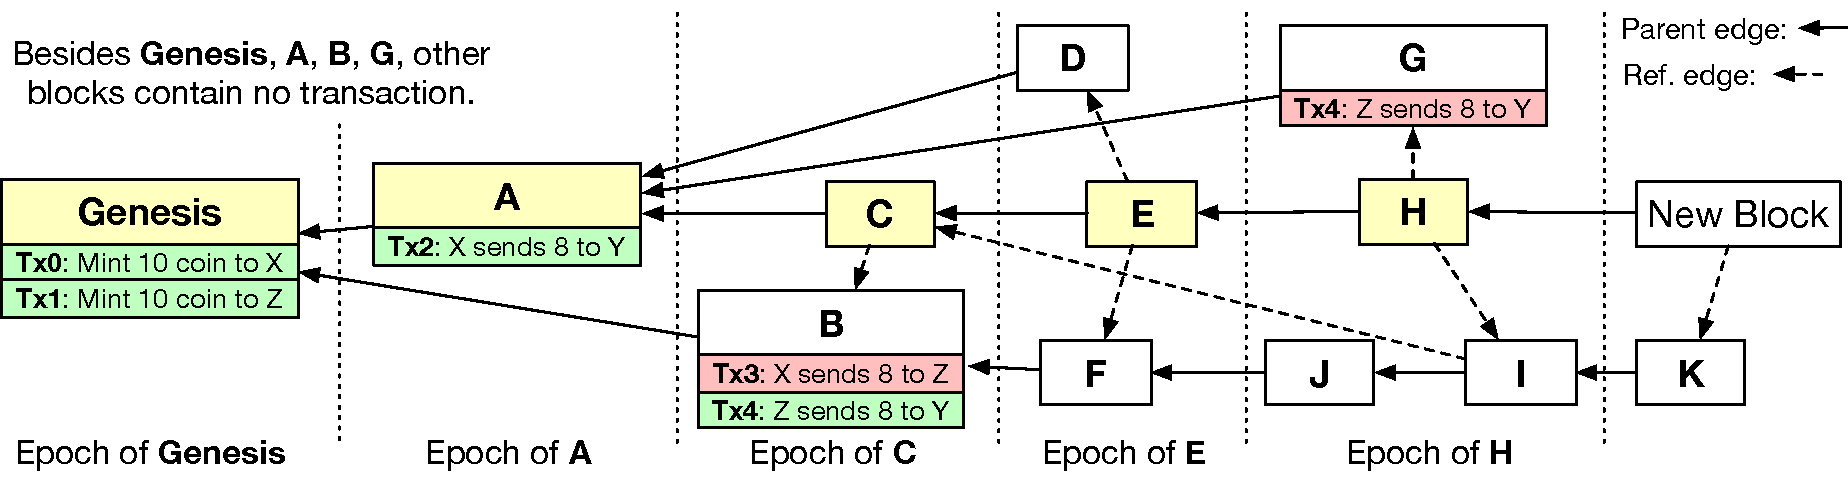
\includegraphics[scale=0.52]{figs/example}
	\caption{An example local \tg state to illustrate the consensus algorithm of
		{\name}. The yellow blocks are on the pivot chain in the \tg. 
		Each block on the pivot chain forms a new epoch to partition
		blocks in the \tg.}
	\label{fig:example}
\end{figure*}




\subsubsection{Epoch}

Given the pivot chain in a \tg,  {\name} splits all blocks into epochs as follows:
\begin{itemize}[nosep]
	\item Every pivot block $\block$ is at epoch $\head(\block)_h$, or simply the \emph{epoch of} $\block$, which is denoted by $\epf(\block)$.
	In particular the genesis block is at epoch $0$.
	      
	\item Every off-pivot block $\block'$ is at the epoch of the first pivot block $\block$ that references it, directly or indirectly. 
	That is, every block $\block'\in \referees(\block)$ is at the epoch of $\block$; then every block $\block''$ referenced by $\block'$, i.e. $\block''\in \referees(\block')\union \set{\parent{\block'}}$, if not already included in an earlier epoch, is also at the epoch of $\block$; and recursively all blocks referenced by $\block''$ and so on.
\end{itemize}

In other words, the epoch of $\block$ consists of all blocks within the local view of $\block$, such that there blocks are potentially produced after $\parent{\block}$ but clearly before $\block$.
% 
For example, 
each of the pivot blocks \phvname{Genesis}, \phvname{A},
\phvname{C}, \phvname{E}, and \phvname{H} corresponds to one individual epoch in Figure~\ref{fig:example}. 
The block \phvname{J} belongs to the epoch of \phvname{H} but not the epoch of \phvname{E}, because \phvname{J} is
reachable from \phvname{H} but not reachable from the previous pivot block \phvname{E}.

It is clear from the definition that as long as the pivot chain is not reverted, the partition of epochs cannot be changed.

\newversion{
\paragraph{Epoch capacity}
	Each epoch now has a limit of executing $200$ blocks. When a single epoch contains more than $200$ blocks, {\name} will only execute the last $200$ blocks (as specified in Section~\ref{sec:total order}) in that epoch. 
	This limit is introduced to battle DoS attacks about releasing a lot of blocks suddenly.
}


\subsubsection{Total Order of Blocks}
\label{sec:total order}

{\name} extends the total order of pivot blocks to all blocks in a \tg as follows.
{\name} first sorts blocks according to their corresponding epochs, so that a block in an earlier epoch always precedes another block in a later epoch;
and then {\name} sorts the blocks inside each epoch based on their topological order, i.e. corresponding to the partial order implied by referee references.
In case two blocks have no partial order relation, {\name} breaks ties deterministically with the unique ids of these two blocks. 
{More detailed rules are described with codes in Figure~\ref{fig:order}.}

\begin{algorithm}[!htb]
	\small
	\SetNlSty{}{}{}
	\DontPrintSemicolon
	\SetKw{To}{ to }
	\SetKw{In}{ in }
	\SetKw{And}{ and }
	\SetKwInOut{Input}{Input}\SetKwInOut{Output}{Output}
	\Input{ A block $\block$ and the local \tg $\graph$ (with $\block$ in $\graph$ and $\gblock$ is the genesis block of $\graph$)}
	\Output{A list of blocks $\mathbf{L} = \block_1 \circ \block_2 \circ \ldots \circ \block_n$, where $\block_1,\dots, \block_n$ are blocks in $\graph$, and in particular $\block_1 = \gblock$ and $\block_n=\block$. \\ A list of pivot blocks $\mathbf{P}=\block'_1\circ\block'_2\circ\cdots\circ\block'_m$ where $\block'_1,\cdots,\block'_m$ are pivot blocks and in particular $\block'_1=\gblock$ and $\block'_m=\block$.}
	\let\oldnl\nl% Store \nl in \oldnl
	\newcommand{\nonl}{\renewcommand{\nl}{\let\nl\oldnl}}% Remove line number for one line
	
	$\block' \longleftarrow \parentf(\block)$\;
	\If {$\mathsf{B}' = \bot$} {
		\Return ($\block$,$\block$)\;
	}
	$(\mathbf{L},\mathbf{P}) \longleftarrow \mathrm{ConfluxOrder}( \block';\graph)$\;
	$\mathbf{L}' \longleftarrow \text{An empty list}$\;
	$\mathsf{\Delta} \longleftarrow \past(\block) \backslash \left(\past(\block') \union \set{\block'}\right)$\;
	\While {$\mathsf{\Delta} \neq \varnothing$} {
		% $\mathsf{\Delta}' \longleftarrow \set{\tilde{\block} \in \mathsf{\Delta} \mid 
		% \forall \ablock\in\mathsf{\Delta}  \left(\tilde{\block}\notin\past(\ablock) \right) }$\;
		% |\future({\tilde \block};\graph)\cap \mathsf{\Delta}| = 0}$\;
		$\mathsf{\Delta}' \longleftarrow \mathsf{\Delta} \backslash\left(\union_{\ablock \in \mathsf{\Delta}} \past(\ablock) \right)$\;

		
		$\block''\longleftarrow {\arg\max}_{\ablock\in\mathsf{\Delta'}}\set{\hash(\ablock)}$\;
		% Let $\block'$ be the block with maximum $\hash(\block')$ in $\mathsf{\Delta}'$\;

		$\mathbf{L}' \longleftarrow \block'' \circ \mathbf{L}'$ \;
		$\mathsf{\Delta} \longleftarrow \mathsf{\Delta} \backslash \set{\block''}$\;
	}
	$\mathbf{L}  \longleftarrow \mathbf{L} \circ \mathbf{L}' \circ \block$\;
	$\mathbf{P} \longleftarrow  \mathbf{P}\circ \block$\;
	\Return $(\mathbf{L},\mathbf{P})$\;
	%\vspace{-2.5mm}
	\caption{The Definition of the $\mathrm{ConfluxOrder}$ function.}
	\label{fig:order}
	%\vspace{-4mm}
\end{algorithm}

For example,  the local \tg in Figure~\ref{fig:example} may give a total order as
\phvname{Genesis}, \phvname{A}, \phvname{B}, \phvname{C}, \phvname{D}, \phvname{F}, \phvname{E}, \phvname{G}, \phvname{J},  \phvname{I}, \phvname{H}, and \phvname{K}.
The order of  \phvname{D} and  \phvname{F} may change if the block id of  \phvname{F} is smaller than  \phvname{D}, 
and the same holds for  \phvname{G}, \phvname{J}, and  \phvname{I}.

\newversion{
	Here we remark that the weight of blocks is not used when extending the pivot chain to the total order of all blocks.
	All blocks, even blocks with zero weight after adaption, are treated equally in this procedure.
}


\subsubsection{Total Order of Transactions}
\label{sec:txorder}
{\name} first sorts transactions based on the relative order of their enclosing blocks.
In case two transactions belong to the same block, {\name} sorts them based on their appearance order in that block.
{\name} checks conflicts of transactions at the same time when deriving
the orders. If two transactions are conflicting with each other, 
e.g. they have exactly the same sender and nonce, 
then {\name} will attempt to execute the first one and 
ignore the second one if the first one is executed. 
If one transaction appears in multiple blocks, {\name}
will keep the first valid appearance of this transaction and discard all redundant ones.

For example, the transaction total order in Figure~\ref{fig:example} is \phvname{Tx0},
\phvname{Tx1}, \phvname{Tx2}, \phvname{\sout{Tx3}}, \phvname{Tx4}, and \phvname{\sout{Tx4}},
where {\name} discards \phvname{Tx3} because it conflicts with
a previously executed valid transaction \phvname{Tx2}, and discards the second appearance of \phvname{Tx4} because it is redundant.


% When the user assumes $q\le 0.25$,
% \begin{displaymath}
% 	n>\min\left\{
% 	\frac{2m}{5}+13,\;
% 	\frac{2m}{7}+36\right\}
% 	\Longrightarrow \risk(\ablock)<10^{-4}
% 	\qquad 
% 	n>\min\left\{
% 	\frac{2m}{5}+19,\;
% 	\frac{2m}{7}+57\right\}
% 	\Longrightarrow \risk(\ablock)<10^{-6}
% \end{displaymath}

% When the user assumes $q\le 0.5$,
% \begin{displaymath}
% 	n>\min\left\{
% 	\frac{2m}{3}+23,\;
% 	\frac{6m}{11}+64\right\}
% 	\Longrightarrow \risk(\ablock)<10^{-4}
% 	\qquad 
% 	n>\min\left\{
% 	\frac{2m}{3}+36,\;
% 	\frac{6m}{11}+103\right\}
% 	\Longrightarrow \risk(\ablock)<10^{-6}
% \end{displaymath}


% %\begin{lemma}
% %\vspace{-2mm}
% Suppose $\block$ is a block on the pivot chain of all honest nodes during the
% time $[t-d, t]$ and $\parentf(\block)$, the parent of $\block$, is generated at time zero. The
% chance of $\block$ being kicked out of the pivot chain by one of its sibling blocks
% $\phvname{A}$ 
% is no more than:
% \begin{displaymath}
% \sum_{k=0}^{n-m}\zeta_k \cdot q^{n-m-k+1} + \sum_{k=n-m+1}^{\infty} \zeta_k
% \end{displaymath}
% where $n$ is the number of blocks in the subtree of $\block$ before time $t-d$, $m$ is the number of blocks in the subtree of $\phvname{A}$ 
% generated by honest nodes, and $\zeta_k = e^{-q\lambda_h t}\frac{(q\lambda_h t)^k}{k!}$.
% %\label{lem:confirm}
% %\vspace{-2mm}
% %\end{lemma}
% This is a direct application of Theorem 10 in \cite{GHOST}.
% It provides us a way to estimate the stability of each individual block on the
% pivot chain. 

% Note that the stability of a pivot
% chain prefix is determined by the least stable block in the prefix.
% %\begin{theorem}
% Suppose $\block$ is a block on the pivot chains of all honest nodes during the time $[t-d, t]$.
% The chance of $\block$ falls off the pivot chain is no more than:
% \begin{displaymath}
% \max_{\substack{\phvname{A}\in \mathrm{Chain}(\block)\\ \phvname{A}'\in \mathrm{Sibling}(\phvname{A})}} \mathrm{Pr}[\text{$\phvname{A}$ is kicked out of the pivot chain by $\phvname{A}'$}]
% \end{displaymath}
%\label{the:confirm}
%\vspace{-4mm}
%\end{theorem}
%Theorem~\ref{the:confirm} indicates that the stability of a pivot
%chain prefix is determined by the least stable block in the prefix. See
%Appendix~\ref{app:proof} for the proof of Lemma~\ref{lem:confirm} and
%Theorem~\ref{the:confirm}.

% \guangsays{List a recommended setting of parameters. Adversary 35\%, $\eps=10^{-80}$ etc.}



% !TEX root = ./tech-specification.tex

%%%%%%%%%%%%%%%%%%%%%%%%%%%%%%%%%%%%%%%%

\newversion{
\subsection{Checkpoint}
\label{sec:checkpoint}

{\name} implements a checkpoint mechanism to tailor the ever-growing blockchain history data.
At a high level, every $\eragap$ epochs form an \emph{era}\footnote{In geologic time scale, \emph{eons} are divided into \emph{eras}, which are in turn divided into \emph{periods}, \emph{epochs} and \emph{ages}.} and a \emph{checkpoint} is made when the era genesis block becomes stable. 
Thereafter, full nodes can safely discard the content of old blocks.
 % as described in Section~\ref{sec:truncate}.
% \todo{ckimpl}{We may not have the following rule currently.}
% blocks in a old era but outside the corresponding checkpoint will be discarded and hence cannot affect future consensus decisions. 
% Thus, once a new checkpoint is made, the full nodes can safely reject unchecked old-era blocks and discard the contents of old blocks (it is suggested but not forced to store the headers of old blocks as a legitimate proof of the current state).


\subsubsection{Era and Era Genesis}

	Formally, eras in {\name} are partitioned with respect to the height of pivot blocks. 
	Every $\eragap$ height corresponds to one era,
	and in particular the pivot block of height $\eragap\cdot N$ is called the \emph{era genesis block of Era $N$}. 
	For example, the genesis block, which is the only block at height $0$, 
	is the era genesis block of Era $0$ (i.e. the first era);
	the pivot block at height $\eragap$ is the era genesis block of Era $1$  (i.e. the second era). 
	Furthermore, an era genesis will eventually be finalized and become a \emph{stable era genesis}, which is irreversible in any case.

	% \subsubsection{Stable Era Genesis}
	% // This is what we called forced confirmation in informal discussion.

	The stable era geneses are recursively defined as below:
	\begin{enumerate}[]
		\item The genesis block is the first stable era genesis.

		\item An era genesis block $\gblock$ becomes a stable era genesis if it satisfies the following:
		% According to the timer chain, the first era genesis block $\gblock$ satisfying the following becomes the next stable era genesis:
		\begin{itemize}[nosep]
			\item $\gblock$ is in the subtree of the last stable era genesis;

			\item the subtree of $\gblock$ contains $\pbeta$ \emph{consecutive} timer blocks ended by $\block$, 
			i.e. $\exists \block$ such that $\block,\parentf_{timer}(\block),\dots,\parentf_{timer}^{(\pbetam)}(\block)$ are all in the subtree of $\gblock$;

			\item there are $\pbeta$ \emph{consecutive} timer blocks in the future of $\block$ (these blocks are not necessarily within the subtree of $\gblock$).
		\end{itemize}

		\item Era genesis blocks preceding a stable era genesis are also stable.
	\end{enumerate}
	 

	Let the latest stable era genesis block of a \tg $\graph$ be denoted by $\mathsf{StableEraGenesis}(\graph)$.
	%
	The GHAST rule, including weight adaption and parent selection (as specified in Section~\ref{subsec:GHAST} and \ref{subsec:GHAST parent}), are applied within the subtree of $\mathsf{StableEraGenesis}(\graph)$. 
	The anti-cone penalty, as defined in Section~\ref{subsec:anticone}, is also subject to blocks within the subtree of $\mathsf{StableEraGenesis}(\graph)$, 
	though such restriction makes no essential difference according to  current anti-cone parameters.




\subsubsection{Truncation of Consensus \tg}\label{sec:truncate}
	
	In a \tg $\graph$, the latest stable era genesis $\mathsf{StableEraGenesis}(\graph)$ is indeed a checkpoint that can be treated as the ``new genesis block'' thereafter, 
	since the consensus rules only apply to blocks within the subtree of $\mathsf{StableEraGenesis}(\graph)$.
	 % and blocks in $\past\left(\mathsf{StableEraGenesis}(\graph)\right)$ cannot be reordered and the total order of transactions is irreversible up to $\mathsf{StableEraGenesis}(\graph)$.
	Therefore, the bodies of blocks in $\past\left(\mathsf{StableEraGenesis}(\graph)\right)$ are no longer needed for future world-states and can be safely discarded from every full node's memory.
	However, the headers of those blocks in $\past\left(\mathsf{StableEraGenesis}(\graph)\right)$ are still needed for validation of references from future blocks (blocks outside the future set $\future\left(\mathsf{StableEraGenesis}(\graph);\graph\right)$ may reference blocks in $\past\left(\mathsf{StableEraGenesis}(\graph)\right)$). 

	For convenience we let $\block'$ and $\block''$ denote the latest two stable era geneses as follows:
	\begin{align*}
		\block' &\eqdef \mathsf{StableEraGenesis}(\graph)\\
		\block'' &\eqdef \mathsf{StableEraGenesis}(\past(\block'))
	\end{align*}

	Blocks missing one stable era genesis, i.e. the blocks in $\future(\block'';\graph)\backslash\future(\block';\graph)$, can be referenced by a new block in $\graph$ but will not affect consensus decision.
	Blocks missing two stable era geneses, i.e. the blocks outside $\future(\block'';\graph)$, cannot be referenced.
	% 
	More specifically, when adding a new block $\block$ into the \tg $\graph$, the validity of $\block$ is examined as follows:
	\begin{enumerate}
		\item If $\block \notin \future(\block'';\graph)$, then $\block$ is discarded.

	    \item If $\block\in \future(\block'';\graph)\backslash\future(\block';\graph)$, 
	    then $\block$ is partially valid.
	    That is, the block $\block$ has zero weight in consensus decision and should not be referenced, but the transactions in $\block_\txs$ are still valid.

	    \item If $\block\in  \future(\block';\graph)$ but
	     % its parent is outside the subtree of $\block''$, i.e. 
	    $\parent{\block} \notin  \mathsf{SubTree}(\block'';\graph)$,
	    then $\block$ is also partially valid.
	  

	    \item Otherwise follow the rules in Section~\ref{sec:pvalid header}.
	\end{enumerate}
}

\subsection{Finalization}

In this part we discuss when a block or a transaction in {\name} is considered irreversible, or ``finalized''.
This is crucial for off-chain users to decide when to confirm a transaction or a state.

Like every other PoW consensus system, the risk that an adversary succeeds in reverting the blockchain history decreases over time but never goes to zero.
That is, there is always a positive probability, no matter how tiny it is, that an adversary generates a branch with higher accumulated weight than the one generated by honest parties.
This is a nature of PoW consensus but not one weakness, because:
1) a sufficiently small probability is usually considered equivalent to zero in practice;
2) that tiny probability can be made even smaller than the probability that an adversary breaks the public-key cryptosystem or finds a collision of the hash reference, and hence not the bottleneck of security.
Therefore, in order to decide the concrete finalization rule, 
a user must specify how much risk he can tolerate as well as his (perhaps subjective) assumption about several system parameters.


In what follows we elaborate the finalization of a block.
A transaction $\tx$ is finalized if the first block $\block'$ where $\tx$ is \textbf{executed} becomes finalized.
This is a sufficient but sometimes not necessary condition\footnote{The finalization of a transaction may be much faster. For example,  a simple transaction $\tx$ may be safely confirmed before the blocks containing $\tx$ being finalized, 
if the execution of $\tx$ is indifferent of the agreement of pivot chain, i.e. no conflicting or dependent transactions of $\tx$ included in competing blocks.}.
Note that ``the first block including $\tx$ becomes finalized'' is insufficient, since {\name} allows invalid transactions.

Consider the block $\block'$ in a \tg and suppose that $\block'$ belongs to the epoch of a pivot block $\block$.
Then the finalization of $\block'$ reduces to the finalization of $\block$ on the pivot chain.
The user can decide whether $\block$ is finalized as follows:
\begin{enumerate}%[nosep]
	\item Estimate or make assumptions about following system parameters:
	\begin{itemize}[nosep]
	 	\item \textbf{Block Generation Rate:} Let $q\eqdef\lambda_a/\lambda_h$ where $\lambda_h$ denotes the combined block generation rate of honest nodes and $\lambda_a$ denotes the block generation rate of attacker. 
	 	The user needs to make an assumption of the attacker's power by setting an upper bound for $q$.

	 	\item \textbf{Network Synchronization:} If at time $t$, an honest node broadcasts a block via the gossip network, then by time $t + d$ all honest nodes receive this block (the nodes not receiving by time $t+d$ will be counted as adversary). 
	 	\newversion{According to our experiment in a globally distributed testing environment, we set $d$ equal to 10 seconds.}
	\end{itemize} 

	\item Make sure that all the pivot blocks preceding $\block$ have been finalized.

	\item Make sure that block $\block$ stays on the pivot chain since $2d$ time ago.

	\item For $q\le 0.2$, compute the confirmation risk $r_1$ according to the \textbf{Fast Confirmation Rule}. 
	\begin{itemize}[nosep]
		\item The fast confirmation rule assumes that the GHAST weight adaption is not triggered under the subtree of $\parent{\block}$ during the generation of $8000$  blocks ($\approx 1.1$ hours) since the creation of $\parent{\block}$.
		% in the next $\approx 1.1$ hours every block $\block'$ under the subtree of $\block$ has normal weight, 
	%% i.e. $\forall \block'$ such that $\block\in\chain(\block')$, there is $\weight(\block')=\block'_d$. 

		\item Let $r_2$ denote the risk that an attacker breaks the above assumption.
	\end{itemize}
	
	
	\item For $q< 1$, compute the confirmation risk $r_3$ according to the \textbf{Slow Confirmation Rule}.

	\item The confirmation risk for $\block$ is bounded as $\risk(\block)\le \min\set{r_1+r_2,r_3}$. 
\end{enumerate}


\subsubsection{Fast/Slow Confirmation Rules}

Since evaluating $\risk(\block)$ may be costly, 
we provide the following simple (but not tight) formulas for risk estimation. 
These estimations are conservative and hence result in a longer confirmation time. 
Users, especially those who are also developers, are encouraged to make more accurate estimation and design sophisticated strategies to achieve a better balance between confirmation time and security. 


For the estimation of confirmation risk, we introduce the following values with respect to the current local \tg $\graph$ and any block $\ablock\in\graph$.

\begin{itemize}[nosep]
	\item $c_0$: the total weight of all blocks locally observable in $\graph$;
	\item $c_1$: the total weight of received blocks in the past $2d$ time (in local clock); 
	\item $\mathbf{d}$ : the largest target difficulty in the last one day (in local clock);

	\item $w_1(\ablock)$: the total weight of blocks under the subtree rooted at $\ablock$ in $\graph$, i.e. $w_1(\ablock)\eqdef \sum_{\ablock'\in \graph: \ablock\in\chain(\ablock')} \weight(\ablock')$;
	\item $w_2(\ablock)$: the maximum weight of subtrees rooted at blocks in $\sible(\ablock)$, i.e. 
	$w_2(\ablock) \eqdef \max_{\ablock'\in \sible(\ablock)} \set{w_1(\ablock')}$ \\
	(here malicious blocks can be excluded for better performance,
	while failing to exclude malicious blocks would result in a correct but more conservative (less accurate) estimation for the upper bound of confirmation risk);

	\item $w_3(\ablock)$: the total weight of all the blocks in $\past(\ablock)$,  i.e. $w_3(\ablock)\eqdef \sum_{\ablock'\in \past(\ablock)} \weight(\ablock')$.
\end{itemize}

 Then we let $n$ be the estimation of $\block$'s advantage over its siblings, and $m$ denote the total (equivalent) number of blocks competing with $\block$, 
 where $n$ and $m$ are formally defined as below:
		\begin{align}
			\label{def:nm}
			n\eqdef \lceil(w_1(\block)-w_2(\block)-c_1)/\mathbf{d}\rceil,
			\;\qquad\;
			m\eqdef\lfloor(c_0-w_3(\parent{\block)})/\mathbf{d}\rfloor
		\end{align}

If $n$ approaches $m$ quickly then it must be the case that most of the mining power are concentrating under the subtree of $\block$,
in which case the block $\block$ can be finalized using the Fast Confirmation Rule.
However, it is possible that the Fast Confirmation Rule is never satisfied for a predetermined risk tolerance in case the convergence of mining power is not that timely.
Then the confirmation of $\block$ has to rely on the Slow Confirmation Rule,
which takes time but will eventually come true as long as the majority of mining power is honest.

\begin{center}
	\begin{threeparttable}
		\caption{The confirmation risk lookup table for Fast Confirmation Rule.}
		\smallskip
		\begin{tabular}{l|ccc}
			\toprule
			Risk tolerance $\backslash$  Adversary power &  
			$q\le 0.1$ (i.e. $9.1\%$ adversary) & $q\le 0.2$ (i.e. $16.7\%$ adversary) \\
			\midrule
			$\risk(\block)<10^{-4}$ & $m-n\le \min\{0.85m-12,4400\}$\tnote{$\ast$} & $m-n\le \min\{0.75m-22,2250\}$ \\
			$\risk(\block)<10^{-6}$ & $m-n\le \min\{0.80m-12,3800\}$ & $m-n\le \min\{0.70m-22,1500\}$ \\
			$\risk(\block)<10^{-8}$ & $m-n\le \min\{0.75m-12,3200\}$  & $m-n\le \min\{0.65m-22,750\}$ \\
			\bottomrule
		\end{tabular}
		\begin{tablenotes}
			\item[$\ast$] Slightly better security than confirmation with $6$ successive blocks in Bitcoin.

			% \item[$\ast\ast$] It is possible that the fast confirmation rule is never satisfied for a predetermined risk tolerance,
			% in which case the block can only be confirmed with the Slow Confirmation Rule.
		\end{tablenotes}
	\end{threeparttable}
\end{center}

\begin{center}	
	\begin{threeparttable}
		\caption{The confirmation risk lookup table for Slow Confirmation Rule.}			
		\begin{tabular}{l|ccc}
			\toprule
			Risk tolerance $\backslash$ Adversary power &  $q\le 0.25$ (i.e. $20\%$ adversary) & $q\le 0.5$ (i.e. $33.3\%$ adversary)&  \\
			\midrule
			$\risk(\block)<10^{-4}$ & $m-n\le 0.6m-5700$\tnote{$\dagger$} & $m-n\le 0.35m-10900$ \\
			$\risk(\block)<10^{-6}$& $m-n\le 0.6m-7200$ & $m-n\le 0.35m-13600$ \\
			$\risk(\block)<10^{-8}$ & $m-n\le 0.6m-8700$ & $m-n\le 0.35m-16200$ \\
			\bottomrule
		\end{tabular}
		\begin{tablenotes}
			\item[$\dagger$] Security equivalent to confirmation with $13\sim 14$ successive blocks in Bitcoin.
		\end{tablenotes}
	\end{threeparttable}
\end{center}	


\paragraph{Safety of Fast Confirmation Rule.}

Now we upper bound the risk $r_2$ that
% a heavy block (with weight $\heavywvalue$ times of usual) is added to the subtree of $\block$ 
% within $8000$ successive blocks since the generation of $\parent{\block}$.
the GHAST weight adaption is triggered within $8000$ successive blocks since the generation of $\parent{\block}$.

Let $h$ be the height of the latest stable era genesis block in the current \tg $\graph$. 
Let $\block_i$ denote the block at height $h+i$ on $\chain(\block)$. 
Let $\psi$ be an arbitrary positive integer (e.g. $\psi=50$).
% 
For integer $j\in\N$, let $m'$ and $m_j,n_j$ be defined as follows: 
\begin{align}
	m' &\eqdef \lfloor (c_0-w_3(\parent{\block}))/\mathbf{d}\rfloor\\
	n_j &\eqdef \lceil(w_1(\block_{(j+1)\cdot \psi})-\max\nolimits_{i\in(j\cdot \psi,(j+1)\cdot \psi]}w_2(\block_i)-c_1)/\mathbf{d}\rceil-m'\\ 
	m_j &\eqdef \lfloor(c_0-w_3(\block_{j\cdot \psi}))/\mathbf{d}\rfloor\;
\end{align}

Let $j_{max}$ be the largest integer satisfying $\mathsf{TimerDis}(\graph,\past(\block_{j_{max}\cdot \psi}))\ge 140$. 
For $q\le 0.2$, the risk $r_2$ is bounded by 
%
\begin{align}
	10^{-7}+\sum_{j=0}^{j_{max}} 10^{(m_j/3-n_j)/700+5.3}
\end{align}

%------------------------------------------------

%%%%%%%%%%%%%%%%%%%%%%%%%%%%%%
%%%%%%  \section{Blockchain Execution}

% !TEX root = ./tech-specification.tex

%%%%%%%%%%%%%%%%%%%%%%%%%%%%%%%%%%%%%%%%

\section{Blockchain Execution}

After determining the total order of blocks, the transactions are executed as if they are packed into sequential blocks on an Ethereum-like chain. 

Blockchain execution is based on a series of ordered blocks $\mathbf{L}$ and a subsequence of pivot blocks $\mathbf{P}$ output by figure~\ref{fig:order}. 
%
The pivot blocks divided into $\mathbf{L}$ into several epochs.  For $k\ge 1$, the epoch $k$ (denoted by $\mathbf{E}_k$) refers the slice in $\mathbf{L}$ started with the next block of $\mathbf{P}[k-1]$ and ended at block $\mathbf{P}[k]$. The epoch 0 refers the genesis block. 


\subsection{Initial state}

{\color{red} This sub-section is a deprecated version.}

The initialization world state $\st^0$ is set as follows. A list $\vec{a}$ with elements $(a,b)$ gives the addresses $a$ and their balance $b$ when the \name blockchain launched.  
\begin{align}
	\forall (a,b)\in \vec{a}, \st^0[a]= \account^0 \quad \mbox{except:} \account_b=b 
\end{align}

% In Oceanus, this list contains the following two addresses for faucet. Each address has initialization balance $5\times 10^{33}$ \unit, i.e., 5000 trillion \coinsign.
% %
% \begin{align*}
% 	\mathsf{0x1be45681ac6c53d5a40475f7526bac1fe7590fb8} \\
% 	\mathsf{0x1e768d12395c8abfdedf7b1aeb0dd1d27d5e2a7f}
% \end{align*}

% The \name internal contracts are also initialized.
% %
% \begin{align}
% 	\forall a\in \{a_{\sf stake},a_{\sf sponsor},a_{\sf admin}\}, \st^0[a] &\eqdef \account^0 \quad \mbox{except:} \account_n=1 \\
% 	\mbox{where:}&\\
% 	a_{\sf admin} &\eqdef \admincontract \\ 
% 	a_{\sf sponsor} &\eqdef \sponsorcontract \\
% 	a_{\sf stake} &\eqdef \stakingcontract
% \end{align}

The global statistic information will be set as follows:

\begin{align}
	\st^0[a_{\sf stake}][k_1]_v & \eqdef \blockinyear\times 2^{80} \\ 
	\st^0[a_{\sf stake}][k_2]_v & \eqdef \blockinyear\times 40000 \\
	\st^0[a_{\sf stake}][k_3]_v & \eqdef 0 \\
	\st^0[a_{\sf stake}][k_4]_v & \eqdef 0 \\
	\st^0[a_{\sf stake}][k_5]_v & \eqdef \sum\nolimits_{(a,b)\in \vec{a}} b \\
	\mbox{where:}&\\
	a_{\sf stake} &\eqdef \stakingcontract \\
	k_1 &\eqdef \sf [accumulate\char`_interest\char`_rate]_{\sf ch} \\ 
	k_2 &\eqdef \sf [interest\char`_rate]_{\sf ch} \\
    k_3 &\eqdef \sf [total\char`_staking\char`_tokens]_{\sf ch} \\
    k_4 &\eqdef \sf [total\char`_storage\char`_tokens]_{\sf ch} \\
    k_5 &\eqdef \sf [total\char`_issued\char`_tokens]_{\sf ch} 
\end{align}


\subsection{Epoch execution}

The blockchain is executed epoch by epoch started with epoch 1. Let $\st_{k-1}$ denote the world state after the execution of epoch $k-1$. The Conflux protocol updates world state from $\st_{k-1}$ to $\st_k$ as follows. Besides updating the world state, the protocol also generates a receipt list $\mathbf{R}_k$ for epoch execution. 

\paragraph{Blocks execution. } First, all the blocks in epoch are executed in sequence by block execution function $\transition_{\sf block}(\st,\block,\mathbf{L}[0..(\tau-1)])=(\st',\mathbf{R}')$, where $\block$ is the block to be executed, $\tau$ is the the index of block $\block$ in $\mathbf{L}$ and $\mathbf{R}'$ is the sequence of transaction receipts. After executing all the blocks, the resultant world-state $\st^*$ becomes the input of the next step and the concatenation of block receipts becomes epoch receipts $\mathbf{R}$. Function $\transition_{\sf block}(\st,\block,\vec{L})$ is defined in section~\ref{sec:block_exec}.

\paragraph{Distribute mining reward. } Since Conflux incentive mechanism puts off the mining reward distribution for $\minerfreeze$ epochs, after execution of epoch $k$, Conflux distribute the mining reward for blocks in $\mathbf{E}_{k-\minerfreeze}$. The computing of mining reward for blocks in epoch $k-\minerfreeze$ requires the following context information.
\begin{itemize}[nosep]
	\item The epoch block set $\mathbf{E}_{k-\minerfreeze}$
	\item The world-state before the execution of all the block $\block$ in $\mathbf{E}_{k-\minerfreeze}$, denoted by $\st(\block)$.
	\item The transaction receipts of all the block $\block$ in $\mathbf{E}_{k-\minerfreeze}$, denoted by $\mathbf{R}'(\block)$.
	\item The tree-graph structure for blocks in $\past(\mathbf{P}[k-\minerfreeze+\anticonecountepoch])$. 
\end{itemize}

Section~\ref{sec:incentive} describes how to compute the block reward $\reward(\block)$ with the context information. The mining reward will be distributed to the block author if the author is . The global parameter \emph{total issued tokens} is updated accordingly. Suppose $\st^*$ is the world state after blocks execution, it will be updated to $\st^{**}$ by
%
\begin{align}
	\st^{**}&\eqdef \st^* \qquad \mbox{except:} \\ 
	\forall a\in \B_{160} \mbox{ with }& \mathsf{Type}_a \in \{[0000]_2,[0001]_2,[1000]_2\} \\ 
	\st^{**}[a]_b&\eqdef \st^*[a]_b +\sum\nolimits_{\block \in \mathbf{E}_{k-\minerfreeze}} \mathbb{I}(\block_{\head_a}=a) \times \reward(\block) \\ 
	\st^{**}[a_{\sf stake}]_{\bf s}[k_3]&\eqdef \st^*[a_{\sf stake}]_{\bf s}[k_3] +\sum\nolimits_{\block \in \mathbf{E}_{k-\minerfreeze}} \left(\mathbb{I}(\mathsf{Type}_{\block_{\head_a}} \in \{[0000]_2,[0001]_2,[1000]_2\} ) \times \reward(\block)-\sum\nolimits_{R\in \mathbf{R}'(\block)}R_f\right) \\ 
	\mbox{where:}&  \\
	a_{\sf stake} &\eqdef \stakingcontract \\ 
	k_3  &\eqdef [{\sf total\char`_issued\char`_tokens}]_{\sf ch}
\end{align}

\subsection{Block execution}\label{sec:block_exec}
The block execution function $\transition_{\sf block}(\st,\block,\vec{L})$ consists of two steps. 

\paragraph{Update accumulate interest}
\begin{align}
	\st^{*}&\eqdef \st \qquad \mbox{except:} \\ 
	\st^{*}[a_{\sf stake}]_{\bf s}[k_1] & \eqdef \left\lfloor\st[a_{\sf stake}]_{\bf s}[k_1] \times \left(1+\frac{4\%}{\blockinyear}\right)\right\rfloor\\
	\mbox{where:}& \\ 
	a_{\sf stake} & \eqdef \stakingcontract \\ 
	k_1 & \eqdef [{\sf accumulate\char`_interest\char`_rate}]_{\sf ch}
\end{align}

\paragraph{Execute transactions in block}

Each block $\block$ contains a series of transactions $\block_{\sf Ts}$. Start with world state $\st^{*}$, \name executes these transactions in sequence by a transform function $\Upsilon(\st,\tx,\vec{L})=(\st',R)$, which updates world state from $\st$ to $\st'$ by processing transaction $\tx$ and outputs a receipt $R$. The input $\vec{L}$ represents the blocks in front of the present block.After executing all the transaction, the resultant state $\st'$ and the concatenation of all the transaction receipts $\mathbf{R}'$ consists of the output of function $\transition_{\sf block}$.


%------------------------------------------------

%%%%%%%%%%%%%%%%%%%%%%%%%%%%%%
%%%%%%  \section{Transaction Execution}


% !TEX root = ./tech-specification.tex

%%%%%%%%%%%%%%%%%%%%%%%%%%%%%%%%%%%%%%%%

\section{交易处理}
%\section{Transaction Processing}
\label{sec:tx_processing}

\name 实现了与以太坊 \cite{ETH_yellow} 相同的虚拟机。
%\name implements the same virtual machine as Ethereum \cite{ETH_yellow}. 
一个交易的执行定义了转换函数 $\Upsilon(\st,\tx,\vec{L})$,其与以太坊的全局状态转换函数类似。
%The execution of a transaction defines the transform function $\Upsilon(\st,\tx,\vec{L})$, which is similar with Ethereum's state transition function.

\subsection{Overview}

在下文中我们将阐述 \name 有关交易执行的具体设计。
%In what follows we focus on the \name specific designs in the execution.

\paragraph{燃料与支付}
\label{subsec:gas_and_pay}

如同第 \ref{sec:tx} 节中的定义样,每笔交易 $\tx$ 的两个域 {\bf 燃料量} 和 {\bf 燃料价格} 标明交易所需燃料 $\tx_g$ 和燃料单位价格 $\tx_p$ 的具体数值。
%As defined in Section~\ref{sec:tx} every transaction $\tx$ has two fields of {\bf gasLimit} and {\bf gasPrice} that declare the specific amount of associated gas $\tx_g$ and the price $\tx_p$ of per unit gas.
开始执行一笔交易 $\tx$ 时,应支付的燃料总价为 $\tx_g \times \tx_p$;当负责支付燃料消耗费用的一方负担不起该费用时,交易 $\tx$ 将被视为无效。
%When starting the execution of a transaction $\tx$, the purchase of gas happens at the price $\tx_g \times \tx_p$ and the transaction $\tx$ is considered invalid if the actor responsible for the cost of gas consumption cannot afford such a purchase.
正常情况下,$\tx$ 的发送方 $\sender{\tx}$ 将承担燃料消耗费用。但燃料消耗可能由交易调用的合约赞助(详见下文)。
%Normally $\sender{\tx}$, the sender of $\tx$, is responsible for the cost of gas consumption. But the gas consumption maybe sponsored by called contract sometimes. (See the following paragraph for details.) 
与以太坊相似,燃料不存在于交易执行过程以外。
%Like in Ethereum, gas does not exist outside the execution of transactions.


未被使用的燃料将在交易 $\tx$ 执行后退回,但退回额度不超过购买燃料所花总价的四分之一。
%The unused gas can be refunded after the transaction $\tx$ is executed, but no more than a quarter of the total value spent on purchasing. 
因此,\emph{可退还燃料量} $g^{\dagger}$ 等于以下两个中更小的值:$\tx$ \textbf{燃料量} 的四分之一和 \emph{合理剩余燃料} $g'$。即,$g^{\dagger}\eqdef \min\set{g', \tx_g/4}$。
%Thus, the \emph{refundable amount of gas} $g^{\dagger}$ is the minimum of the \emph{legitimately remaining gas} $g'$ and a quarter of the \textbf{gasLimit} of $\tx$,i.e. $g^{\dagger}\eqdef \min\set{g', \tx_g/4}$, 
特别地,若发送方导致 $\tx$ 执行失败,则理论上没有燃料可退还(即 $g^{\dagger} = g' = 0$)。
%where in principle no gas is refundable (i.e. $g^{\dagger} = g' = 0$) if the execution of $\tx$ fails due to the sender's fault. 
最初为 $\tx$ 购买燃料的一方将收到退款 $g^{\dagger}\times\tx_p$。而支付给已消耗燃料的 \coinsign 为
%The actor who initially purchased the gas for $\tx$ will get the refund of $g^{\dagger}\times\tx_p$. And the \coinsign paid for the consumed gas is 
	%
\begin{align}
	\left(\tx_g-g^{\dagger}\right)\times \tx_p.
\end{align}
	%
如果 $\tx$ 未被执行(即,如第 \ref{sec:tx validate} 中定义一般,仅当 $R_z=2$ 时),没有燃料需要被支付。
	%If the $\tx$ is not executed (i.e. only when $R_z=2$ as in Section~\ref{sec:tx validate})), no gas will be charged. 
若发送方 $\sender{\tx}$ 无法负担燃料费,发送方的全部余额将被用于支付燃料费,此实际收取的燃料费将被记录在收据 $R_f$ 中。
	%If the sender $\sender{\tx}$ can not afford gas fee, all its the remained balance of sender $\sender{\tx}$ will be charged as gas fee. The actual charged gas fee will be record in receipt $R_f$. 


支付完毕的燃料费将加入矿工奖励池。因此,更高的燃料价格使发送者花费更多的同时,也将增加该交易被及时处理的概率。
%The charged gas fee is added to the reward pool for miners. Thus in general a higher gas price on a transaction would cost the sender more but also increase the chance of being processed timely.


计算整个区块的累计燃料消耗时,不可退还的燃料 $g^{\dagger} - g'$ 将不被纳入考量。
%In computing the accumulated gas used of the whole block, the non-refundable gas $g^{\dagger} - g'$ is not taken into consideration. 
但当发送方 $\sender{\tx}$ 无法负担燃料费时,即使实际收取的燃料费少于 $\tx_p\times\tx_g$,我们也认为消耗的燃料量即是 $\tx_g$。
%But in case the sender $\sender{\tx}$ can not afford gas fee, the gas used is considered as $\tx_g$, even if the actual charged gas fee is less than $\tx_p\times\tx_g$. The gas used is also recorded in receipt $R_g$. 

\paragraph{存储上限和存储抵押}
%\paragraph{Storage Limit and Storage Collateral}

每笔交易都有一个 \textbf{存储上限} 域,表明当前交易可增加的最大存储字节 $\tx_\ell$。
%Every transactions also have a filed of \textbf{storage limit} that declare the maximum storage bytes $\tx_\ell$ increasing for the present transaction. 
执行交易前,除燃料费用和转账额以外,发送方 $\sender{\tx}$ 必须有足够余额为所需 \textbf{存储上限} 支付存储抵押,即 $\tx_\ell\times\collateralperbyte\;\unit$。
%Before transaction execution, besides gas fee and transferred value, the sender $\sender{\tx}$ must have enough balance for storage collateral for specified \textbf{storageLimit}, i.e., $\tx_\ell\times\collateralperbyte\;\unit$. 
不同于燃料费,在执行交易前这些抵押将不被收取或锁定。
%Unlike the gas fee, these collateral will not be charged or locked at this time. 
在交易执行完成时,若发送方没有足够余额为实际增加的存储支付抵押,或实际增加的存储字节超过了存储上限,交易执行将失败。
%At the end of transaction execution, if the sender doesn't have enough balance paying for the increased storage collateral or the increased storage bytes of sender exceeds storage limit, the transaction execution fails. 
更多有关存储抵押的细节详见第 \ref{sec:collateral} 节。
%More details for collateral for storage is specified in section~\ref{sec:collateral}. 

\paragraph{赞助}
%\paragraph{Sponsorship}

当交易 $\tx$ 调用一个带有 \textbf{燃料资助人} 的智能合约 $\contract$,且 $\tx$ 满足 \cref{eq:whitelist} 中定义的函数 $\mathsf{Whitelist}(\cdot)$ 要求而有资格使用该赞助时,
%In case the transaction $\tx$ is calling a smart contract $\contract$ with \textbf{sponsor for gas} and $\tx$ is qualified for the subsidy as checked in function $\mathsf{Whitelist}(\cdot)$ defined in \cref{eq:whitelist}, 
若 $\contract$ 有足够的 \textbf{燃料资助余额} 且交易 \textbf{燃料上限} $\tx_g$ 不超过 {\bf 燃料资助上限},
$\contract$ 将负责购买燃料;
%$\contract$ is responsible for the purchase of gas if it has sufficient \textbf{sponsor balance for gas} and the transaction \textbf{gasLimit} $\tx_g$ does not exceed the {\bf sponsor limit for gas}, 
否则,交易发送方 $\sender{\tx}$ 仍负责购买燃料全额。
%and otherwise the sender $\sender{\tx}$ is still responsible for the whole purchase of gas as if there were no sponsor at all. 
我们正式定义函数 $\mathsf{GasElig}(\st,\tx)$ 来检查交易 $\tx$ 是否有资格使用燃料赞助,同时定义 $\mathsf{GasSpr}(\st,\tx)$ 来检查实际上 $\tx$ 是否使用了燃料赞助。
%Formally, we define function $\mathsf{GasElig}(\st,\tx)$ to check whether transaction $\tx$ is eligible for gas consumption sponsorship and define function $\mathsf{GasSpr}(\st,\tx)$ to check whether $\tx$ is actually sponsored for gas consumption. 
\begin{align}
\mathsf{GasElig}(\st,\tx)&\eqdef \quad \mathrm{Type}_{\tx_a}=\typecontract \;\wedge\; \mathsf{Whitelist}(\st,\sender{\tx},\contract) \;\wedge\; \st[\tx_a]_p[\mathsf{gas}]_a\neq 0 \;\wedge\; \tx_g\times\tx_p \le \st[\tx_a]_p[\mathsf{limit}] \\
\mathsf{GasSpr}(\st,\tx) &\eqdef\quad  \mathsf{GasElig}(\st,\tx) \;\wedge\; \st[\tx_a]_p[{\sf gas}]_b\ge \tx_g\times\tx_p
\end{align}
%
其中,函数 $\mathsf{Whitelist}(\cdot)$ 在 \cref{eq:whitelist} 有详细定义。
%where function $\mathsf{Whitelist}(\cdot)$ is defined in \cref{eq:whitelist}. 

若一个合约存在 \textbf{存储抵押资助人}, 存储抵押费用也能被合约赞助。正式定义下,
%If a contract has \textbf{sponsor for collateral}, the storage collateral can also be sposnored by a contract. Formally,
\begin{align}
\mathsf{ColElig}(\st,\tx) &\eqdef \quad \mathrm{Type}_{\tx_a}=\typecontract \;\wedge\; \mathsf{Whitelist}(\st,\sender{\tx},\contract) \;\wedge\; \st[\tx_a]_p[\mathsf{col}]_a\neq 0 \\
\mathsf{ColSpr}(\st,\tx) &\eqdef\quad  \mathsf{ColElig}(\st,\tx) \;\wedge\; \st[\tx_a]_p[{\sf col}]_b\ge \tx_\ell\times \collateralperbyte
\end{align}

\subsection{交易执行}
%\subsection{Transaction Execution}

\subsubsection{执行前验证}
%\subsection{Pre-execution Validation}
\label{sec:tx validate}

在被执行前,一笔处于待执行列中的交易 $\tx$ 必须通过以下有关交易合法性的第二轮测试:
%Before being executed, a transaction $\tx$ in the processing queue must pass the following secondary test of intrinsic validity. 
\begin{enumerate}[nosep]
	\item 当前纪元处于 \textbf{epochHeight} 所指明的区间之内,即当前纪元高度在 $[\tx_e - \txepochbound, \tx_e + \txepochbound]$ 之间。
	%\item The current epoch is in the range specified by \textbf{epochHeight}, i.e. current epoch height is in $[\tx_e - \txepochbound, \tx_e + \txepochbound]$.
	
	\item 交易 \textbf{序列号} 合法,即 $\tx_n = \st\left[\sender{\tx}\right]_n$,其中 $\st$ 表示当前世界状态。
	%\item The transaction \textbf{nonce} is valid, i.e. $\tx_n = \st\left[\sender{\tx}\right]_n$ where $\st$ is the current world-state.

	\item 接收方地址合法,即 $\tx_a$ 的(前 $4$ 位)类型标志属于 $\set{\typereserved,\typenormal,\typecontract}$。
    %\item The recipient address is valid , i.e. the type indicator (first $4$-bit) of $\tx_a$ belongs to $\set{\typereserved,\typenormal,\typecontract}$.
\end{enumerate}

需要注意的是交易的本地合法性,即 $\rlp$ 格式和签名有效性,
%Note that the local legality of the transaction, e.g. the $\rlp$ format and the validity of signature, 
已在有关交易合法性的第一轮测试中(定义见第 \ref{sec:block validate} 节)得到验证。第一轮测试在将相应区块纳入 \name 树图时进行,因此在第二轮测试中本地合法性将不被二次检查。
%is already verified in the first intrinsic validity test before accepting the corresponding block into the \name \tg, as discussed in Section~\ref{sec:block validate}, and will not be checked again at this moment.

若 $\tx$ 未能通过这些检查,系统将不执行该交易,不增加账户序列号,也不对此交易收取交易费用。
%If $\tx$ fails at these checks, the transaction will not be executed, the nonce for account will not increase and no transaction fee is charged for such transaction. 
用 $R'$ 表示前一笔交易的收据,
%Let $R'$ be the receipt of last transaction.
则当前交易的收据将被设为:
%Then the receipt of current transaction will be set as follows:
\begin{align}
	R_u=R'_u && R_f=0 && R_g=0 && R_{\bf l}=\emptystring && R_z=2 && R_s=0 && R_{\bf o}=\emptystring && R_{\bf i}=\emptystring
\end{align}
%
布隆过滤器 $R_b$ 根据日志 $R_{\bf l}$ 计算而已。
%(The bloom filter $R_b$ of log $R_{\bf l}$ is computed accordingly. )

若 $\tx$ 通过了以上交易前检查,$\tx$ 的执行过程如本节余下内容所述。
%If $\tx$ passes all the above pre-execution checks, the execution of $\tx$ is as specified in the rest of this section.


\subsubsection{预处理}
%\subsubsection{Preprocessing}
\label{subsubsec:preprocessing}

在 $\tx$ 的预处理阶段,为确保未来成功操作,$\sender{\tx}$(或资助人) 的余额将被检查。
%In the preprocessing phase of $\tx$, the balance of $\sender{\tx}$ (and the sponsor, if applicable) is examined so that the payment for any further operation is assured.
若 $\tx$ 通过了预处理,世界状态将从 $\st$ 转变为 $\st^0\eqdef \st^{**}$;否则,世界状态将变为 $\st'$,而交易 $\tx$ 的执行将被中止。
%The world-state will be transformed from $\st$ into $\st^0\eqdef \st^{**}$ if $\tx$ passes the preprocessing, or directly into $\st'$ and the execution is aborted if $\tx$ fails at any step.

\paragraph{序列号增加}
%\paragraph{Nonce incremental.}
交易执行的开始将对世界状态 $\st$ 产生一个不可更改的变动:
%The beginning of execution causes an irrevocable changed to the state $\st$: 
发送方的账户序列号 $\sender{\tx}_n$ 将增加一。
%the nonce of the sender, $\sender{\tx}_n$, is incremented by one. 
%
世界状态 $\st^*$ 的定义如下:
%We define the state $\st^*$:
\begin{align}
	\st^*  &\eqdef \st \qquad \mbox{  except:}\\
	\st^*\left[\sender{\tx} \right]_n &\eqdef \st\left[\sender{\tx} \right]_n+1 
\end{align}

\paragraph{燃料消耗支付验证}
%\paragraph{Gas consumption payment validation.}

进行交易 $\tx$ 的提前支付时,系统首先明确燃料消耗是否有赞助。
%The up-front payment of a transaction $\tx$ first figures out whether the gas consumption is sponsored. 
若 $\tx$ 有资格使用燃料赞助,且其调用的合约有足够的 \textbf{燃料资助余额},则交易 $\tx$ 有燃料赞助。
%$\tx$ is sponsored on gas consumption if $\tx$ is eligible for sponsorship on gas consumption and the calling contract has sufficient \textbf{sponsor balance for gas fee}. 
\begin{itemize}
	\item 若 $\tx$ 的燃料消耗使用了赞助,燃料费支付后的世界状态 $\st^{**}$ 定义如下:
	%\item If the gas consumption of $\tx$ is sponsored, the world-state $\st^{**}$ after gas consumption payment is as follows: 
	\begin{align}
		\st^{**}  &\eqdef \st^* \qquad \mbox{  except:}\\
		\st^{**}\left[\contract_{addr}\right]_p[{\sf gas}]_b &\eqdef \st^*\left[I_a\right]_p[{\sf gas}]_b-\tx_g\times\tx_p
	\end{align} 
	
	\item 否则,发送方 $\sender{\tx}$ 需支付燃料费。
	%\item Otherwise, the sender $\sender{\tx}$ is required to pay for the gas consumption. 
	$\sender{\tx}$ 的余额应满足 $\st^{*} \left[\sender{\tx}\right]_b \ge \tx_g\times\tx_p+\tx_v$;否则,系统将生成一个 \emph{余额不足例外}。
	%The balance of $\sender{\tx}$ should satisfy $\st^{*} \left[\sender{\tx}\right]_b \ge \tx_g\times\tx_p+\tx_v$ and otherwise a \emph{not enough balance exception} is generated. 
	处理此 \emph{余额不足例外} 的方法将在之后讨论。
	%The handling of \emph{not enough balance exception} will be discussed later.
	燃料费支付后的世界状态定义如下:
	%The world-state after the gas consumption payment is defined as: 
	\begin{align}
		\st^{**}  &\eqdef \st^* \qquad \mbox{  except:}\\
		\st^{**} \left[\sender{\tx}\right]_b &\eqdef \max\set{\st^*\left[\sender{\tx}\right]_b-\tx_g\times\tx_p,0}
	\end{align}
\end{itemize}

\paragraph{存储上限验证}
%\paragraph{Storage limit validation.}

确定燃料费用后,Conflux 将决定由谁来支付存储抵押。
%After charging, Conflux decides who is responsible for storage collateral. 
若 $\tx$ 有资格使用存储抵押赞助,且被调用的合约 $\contract=\tx_a$ 有充足的 \textbf{存储抵押资助余额},则合约 $\contract$ 将负责支付由执行 $\tx$ 产生的存储抵押,并成为修改项的所有者。
%If $\tx$ is eligible for sponsorship on storage collateral and calling contract $\contract=\tx_a$ has enough \textbf{sponsor balance for collateral}, contract $\contract$ is responsible for the storage collateral resulted in the execution of $\tx$ and will be the owner of modified entries. 
%
否则,发送方 $\sender{\tx}$ 为修改项的所有者,并有义务支付相应的存储抵押。
%Otherwise, the sender $\sender{\tx}$ is the owner of modified entries and has the obligation to pay corresponding storage collateral. 
%
\begin{align}
	\mathsf{ColOwner}(\st,\tx) &\eqdef\left\{ \begin{array}{ll}
		\tx_a & \text{if } \mathsf{ColSpr}(\st,\tx) = \true \\ 
		\sender{\tx} & \text{if } \mathsf{ColSpr}(\st,\tx) = \false \\ 
	\end{array}\right.
\end{align}

若 $\sender{\tx}$ 是存储所有者,但其账户在转帐 $\tx_v$ 后无法负担 {\bf 存储上限} 所标明的抵押全额,
%If $\sender{\tx}$ is the storage owner but his balance cannot afford the full collateral as declared in {\bf storageLimit} after transferring value $\tx_v$, 
即 $\st^{**}[\sender{\tx}]_b<\tx_v+\tx_\ell\times 10^{18}/1024$,
%i.e. $\st^{**}[\sender{\tx}]_b<\tx_v+\tx_\ell\times 10^{18}/1024$, 
那么 $\tx$ 的执行将因为 \emph{余额不足例外} 失败。
%then the execution of $\tx$ fails due to \emph{not enough balance exception}. 

\paragraph{处理余额不足例外} 
%\paragraph{Handling not enough balance exception.} 

每当 $\tx$ 在预处理过程中生成一个 \emph{余额不足例外} 时,$\tx$ 的执行将失败,且 $\tx$ 将不继续执行。
%Whenever the preprocessing of $\tx$ generates a \emph{not enough balance exception} during preprocessing, the execution of $\tx$ fails and there will be no further execution of $\tx$. 
为明确该例外是否由合约的赞助余额不足造成,交易执行前的发送方账户余额(即 $\st[\sender{\tx}]_b$)将与一个 \emph{最低要求余额(minimum required balance)} 做比较。该 \emph{最低要求余额} 定义如下: 
%To figure out whether this exception caused by the insufficient sponsorship balance in contract, the sender balance before transaction execution (i.e. $\st[\sender{\tx}]_b$) is compared with a \emph{minimum required balance} defined as
\begin{align}
	\tx_v+(1-\mathbb{I}(\mathsf{GasElig}(\st,\tx)))\times \tx_g \times \tx_p + (1-\mathbb{I}(\mathsf{ColElig}(\st,\tx)))\times \tx_\ell \times \collateralperbyte.
\end{align}

若 $\st[\sender{\tx}]_b$ 大于 \emph{最低要求余额},系统将认定 \emph{余额不足例外} 不因发送方 $\sender{\tx}$ 而产生。
%If $\st[\sender{\tx}]_b$ has enough balance for \emph{minimum required balance}, the sender $\sender{\tx}$ is considered not responsible for the generated \emph{not enough balance exception}. 
这种情况下,例外所造成的世界状态 $\st'$ 将被恢复为 $\st$;为使 $\tx$ 可被再次使用,发送方的账户序列号将被重设
%In this case, the resultant world-state $\st'$ is reverted to $\st$, the nonce of sender is reset so that $\tx$ is reusable. 
收据由以下项组成(其中 $R'$ 表示上一笔交易的收据):
%The receipt is composed as follows (where $R'$ refers the receipt of last transaction):
\begin{align}
	&R_u=R'_u && R_f=0 && R_g=0 && R_{\bf l}=\emptystring \\
	&R_z=2 && R_s=0 && R_{\bf o}=\emptystring && R_{\bf i}=\emptystring
\end{align}

其他情况下,例外因发送方 $\sender{\tx}$ 而产生。
%In other cases, sender $\sender{\tx}$ is responsible for the exception. 
例外所造成的世界状态将从 $\st'$ 恢复为 $\st^{**}$。若发送方存在(即 $\st[\sender{\tx}]\neq\varnothing$),则收据由以下项组成:
%The resultant world-state is $\st'$ is reverted to $\st^{**}$ and the receipt is composed as follows if sender is non-existent. (i.e. $\st[\sender{\tx}]\neq\varnothing$).
\begin{align}
	&R_u=R'_u+\tx_g && R_f=\min\{\tx_g\times\tx_p,\st[\sender{\tx}]_b\} && R_g=\mathsf{GasElig}(\st,\tx) && R_{\bf l}=\emptystring \\
	&R_z=1 && R_s=0 && R_{\bf o}=\emptystring && R_{\bf i}=\emptystring
\end{align}

若例外因发送方 $\sender{\tx}$ 而产生,且发送方不存在,例外所造成的世界状态将从 $\st'$ 恢复为 $\st$,收据如下:
%If sender $\sender{\tx}$ is responsible for the exception and the sender is empty, the resultant world-state is $\st'$ is reverted to $\st$. The receipt is composed as follows
\begin{align}
&R_u=R'_u && R_f=0 && R_g=0 && R_{\bf l}=\emptystring \\
&R_z=2 && R_s=0 && R_{\bf o}=\emptystring && R_{\bf i}=\emptystring
\end{align}


\subsubsection{执行子状态}
%\subsubsection{Execution Substate}
\label{subsubsec:substate}

\emph{交易子状态} $A$ 是一个在执行中积累中间信息的三元组。
%The \emph{transaction substate} $A$ is a three tuple which accrues intermediate information during execution. 
\begin{align}
	A\eqdef \left( A_{\bf s}, A_{\bf l}, A_{\bf c}\right)
\end{align}
$A$ 的组成部分定义如下:
%The components of $A$ are defined as follows: 
\begin{itemize}[nosep]
	\item $A_{\bf s}$ 是一个边执行边自毁的账户集合,在交易完成时其将被遗弃。
	%\item $A_{\bf s}$ is the self-destruct set of accounts that will be discarded upon the transaction's completion.

	\item $A_{\bf l}$ 是一个虚拟机代码执行中产生的可索引日志序列,其允许轻量级客户端追踪一个合约的执行。
	%\item $A_{\bf l}$ is the log series consisting of indexable ``checkpoints'' in the VM code execution, allowing light clients to track the execution of a contract.

	\item $A_{\bf c}$ 是一个键值对集合,记录着每个地址的存储抵押变化值。与世界状态相似,我们用 $A_{\bf c}[k]=\varnothing$ 表示键 $k$ 不存在的情况,并使用 $A_{\bf c}[k]=0$ 简代 $A_{\bf c}[k]=\varnothing$。
	%\item $A_{\bf c}$ is the set of key-value pairs for the storage collateral changes for each address. Similar with the world state, we write $A_{\bf c}[k]=\varnothing$ for the case that the key $k$ does not exist and regard $A_{\bf c}[k]=\varnothing$ as $A_{\bf c}[k]=0$.

	%\item $A_{\bf t}$ 是一个交易所涉及账户的集合,其中空账户将在交易完成时被删除。
	%\item $A_{\bf t}$ is the set of touched accounts, of which the empty ones will be deleted on the transaction's completion.
\end{itemize}

空白的子状态 $A^0$,也即初始子状态,没有账户自毁记录、日志,和所涉及账户记录。$A^0$ 的正式定义为
%The empty substate $A^0$, which is also the initial substate, has no self-destructs, no logs, no touched accounts, and zero refund. Formally, $A^0$ is defined as
\begin{align}
	A^0\eqdef \left( \varnothing, \emptystring, \varnothing\right)
\end{align}

对任意两个子状态 $A^1$ 和 $A^2$,两者累计的子状态 $A\eqdef A^1\Cup A^2$ 定义如下:
%For any two substate $A^1$ and $A^2$, the accrued substate $A\eqdef A^1\Cup A^2$ is defined by 
\begin{align}
	A_{\bf s} &\eqdef A^1_{\bf s} \cup A^2_{\bf s} \\ 
	A_{\bf l} &\eqdef A^1_{\bf l} \cdot A^2_{\bf l} \\
	\forall a\in\B_{160},\; A_{\bf c}[a] & \eqdef A^1_{\bf c}[a]+A^2_{\bf c}[a]
	% A_{\bf t} &\eqdef A^1_{\bf t} \cup A^2_{\bf t} 
\end{align}


\subsubsection{类型依存性执行}
%\subsubsection{Type dependent execution}

若交易通过了预处理阶段,
%If transaction passes the preprocessing, 
{\name} 将根据 \emph{执行前临时状态} $\st^0$ 评估其 \emph{执行后临时状态} $\st^P$。
而\emph{执行前临时状态} $\st^0$ 取决于 $\tx_a$ 所明确的交易类型:创建合约或消息调用。
%then {\name} evaluates the \emph{post-execution provisional state} $\st^P$ from \emph{pre-execution provisional state} $\st^0$ depending on the transaction type as specified in $\tx_a$: either contract creation or message call. 
%
下一步计算可用的燃料为 $g\eqdef \tx_g-g_0$,其中 $g_0$ 表示 $\tx$ 的内在成本(定义见 \ref{def:g0})。
%The gas available for the proceeding computation is $g\eqdef \tx_g-g_0$, where $g_0$ is the intrinsic cost of $\tx$ as in (\ref{def:g0}). 

我们定义一个包含执行后临时状态 $\st^{P}$ ,剩余燃料 $g$,累计子状态 $A$,和状态代码 $z$ 的多元组:
%We define the tuple of post-execution provisional state $\st^{P}$, remaining gas $g$, accrued substate $A$ and status code $z$:
\begin{align}\label{def:transform}
	(\st^{P},g',A,z)\eqdef
	\begin{cases}
		\creation(\st^0,\sender{\tx},\sender{\tx},\emptystring, \mathsf{ColOwner}(\st,\tx),g,\tx_p,\tx_v,\tx_{\bf i},0,\zeta,\top) &  \tx_a=\varnothing \\
		\execution(\st^0,\sender{\tx},\sender{\tx},\tx_a,\emptystring,\mathsf{ColOwner}(\st,\tx),\tx_a,g,\tx_p,\tx_v,\tx_v,\tx_{\bf d},0,\top) & \tx_a\neq\varnothing
	\end{cases}
\end{align}
%
需要注意的是,与以太坊相比我们多了三个参数。
%Notice that we have three more parameters compared with Ethereum. 

函数 $\creation$ 和 $\execution$ 的规范分别在第 \ref{sec:creation} 节和第 \ref{sec:execution} 节有所说明。
%The specifications of function $\creation$ and $\execution$ are given in Section~\ref{sec:creation} and Section~\ref{sec:execution} respectively.

\subsubsection{后处理}\label{sec:tx_post_process}
%\subsubsection{Postprocessing}\label{sec:tx_post_process}

\paragraph{存储抵押退款及收费}
%\paragraph{Storage collateral refund and charge.}

在处理消息调用或合约创建请求后,Conflux 检查增加的存储是否超过 $\tx_\ell$ 中所规定的存储上限,以及存储项所有者是否有足够余额支付存储抵押。
%After the message call or contract creation is processed, Conflux checks whether the incremental storage exceeds storage limit specified in $\tx_\ell$ and if the storage owner has enough balance for storage collateral. 
我们用 $i\eqdef \mathsf{ColOwner}(\st,\tx)$ 表示修改后存储项的所有者地址,并用 $v$ 表示可用于支付存储抵押的余额,其定义如下:
%Let $i\eqdef \mathsf{ColOwner}(\st,\tx)$ be the address who owns modified storage entries and $v$ be the available balance to pay for storage collateral, which is defined as 
\begin{align}
	v \eqdef \begin{cases}
		\st^{P}[\sender{\tx}]_b & \text{if }\mathsf{ColSpr}(\st,\tx)=\false \\
		\st^{P}[\tx_a]_p[{\sf col}]_b &  \text{if }\mathsf{ColSpr}(\st,\tx)=\true
	\end{cases}
\end{align}
%
需要注意的是,$A_{\bf c}[i]$ 是在执行过程中增加的存储抵押。
%Notice that $A_{\bf c}[i]$ is the incremental storage collateral during execution.
若 $A_{\bf c}[i]>\min\{v,\tx_\ell\times 10^{18}/1024\}$,执行将因为抵押余额不足或超出存储上限而失败,
%If $A_{\bf c}[i]>\min\{v,\tx_\ell\times 10^{18}/1024\}$, then the execution fails because of not enough balance for collateral or exceeding the storage limit, 
且所有经过修改的状态将被恢复至 $\st^0$,即 $\st'\eqdef\st^0$。
%and all the modified state will be reverted to $\st^0$, i.e. $\st'\eqdef\st^0$. 
我们用 $R'$ 表示上一笔交易的收据,则此情况下当前交易 $\tx$ 的收据为
%Let $R'$ denote the receipt of last transaction. Then the receipt of current transaction $\tx$ will be 
\begin{align}
	&R_u=R'_u+\tx_g && R_f = \tx_g\times\tx_p && R_g = \mathsf{GasSpr}(\st,\tx) && R_{\bf l}=\emptystring \\
	&R_z=1 && R_s = \mathsf{ColSpr}(\st,\tx) && R_{\bf o}=\emptystring && R_{\bf i}=\emptystring
\end{align}

否则,\name 收取并在后续退还存储抵押,将世界状态 $\st^P$ 转化为 $\st^*$/
%Otherwise \name charges and refunds storage collateral and transforms world-state $\st^P$ into $\st^*$. 
我们在此略过边执行边自毁合约,因为其存储抵押在自毁过程中已被退还。
%We skim the self-destructed contracts here because their storage collateral have been refunded during self-destruction. 
此时,账户状态中的存储抵押也将被更新。
%The storage collateral in account state is also updated at this time. 

\begin{align}
	&\st^1  \eqdef \st^{P} \qquad \mbox{  except:}\\
	&\forall a \in \B_{160} \text{ with }  A_{\bf c}[a]\neq 0, \\
	&\quad \begin{cases}
	\st^1[a]_p[{\sf col}]_b \eqdef \st^{P}[a]_p[{\sf col}]_b + f(a) & \mbox{if $a$ refers to a contract account, i.e. $\mathsf{Type}_{a}=\typecontract$} \\
	\st^1[a]_b \eqdef \st^{P}[a]_b + f(a) & \mbox{if $a$ refers to a normal account, i.e. $\mathsf{Type}_{a}= \typenormal$}
	\end{cases}\\
	& \st^1[a]_o \eqdef \st^P[a]_o - f(a)\\ 
	&\st^1[a_{\sf stake}]_{\bf s}[k_3] \eqdef \st^P[a_{\sf stake}]_{\bf s}[k_3] + \sum_{a\in \B_{160}}(f(a) + A_{\bf c}[a]) \\
	&\st^1[a_{\sf stake}]_{\bf s}[k_4] \eqdef \st^P[a_{\sf stake}]_{\bf s}[k_4] + \sum_{a\in \B_{160}}A_{\bf c}[a] \\
	&\mbox{where:}  \\
	&a_{\sf stake} \eqdef \stakingcontract \\ 
	&k_3 \eqdef {\sf [total\char`_issued\char`_tokens]_{\sf ch}}  \\ 
	&k_4 \eqdef {\sf [total\char`_storage\char`_tokens]_{\sf ch}}  \\ 
	& f(a) \eqdef \min\{-A_{\bf c}[a], \st^P_o[a]\}
\end{align}

\paragraph{燃料费退款}
%\paragraph{Gas fee refund.}

\emph{可退还燃料量} $g^{\dagger}$ 是以下两个中更小的值:$\tx$ \textbf{燃料量} 的四分之一和 \emph{合理剩余燃料} $g'$。即,$g^{\dagger}\eqdef \min\set{g', \tx_g/4}$。
%The \emph{refundable amount of gas} $g^{\dagger}$ is the minimum of the \emph{legitimately remaining gas} $g'$ (as calculated in (\ref{def:transform})) and a quarter of the \textbf{gasLimit} of $\tx$, i.e. $g^{\dagger}\eqdef \min\set{g', \tx_g/4}$.
燃料费退款作用于世界状态 $\st^{*}$,并使 $\st'\eqdef \Upsilon(\st,\tx)$。
%The refund of gas fee is applied on world-state $\st^{*}$ and results in $\st'\eqdef \Upsilon(\st,\tx)$.

\begin{align}
	& \st^2  \eqdef \st^1 \qquad \mbox{  except:}\\
	& \quad \begin{cases} 
		\st^2\left[\tx_a\right]_p[{\sf gas}]_b \eqdef \st^1\left[\tx_a\right]_p[{\sf gas}]_b+g^{\dagger}\times \tx_p 
		& \mbox{if $\mathsf{GasSpr}(\st,\tx)=\true$}\\
		\st^2 \left[\sender{\tx}\right]_b \eqdef \st^1\left[\sender{\tx}\right]_b + g^{\dagger}\times \tx_p 
		& \mbox{if $\mathsf{GasSpr}(\st,\tx)=\false$}
	\end{cases} 
\end{align}

\paragraph{Killed contract processing} 
%\paragraph{Killed contract processing} 

赞助机制和抵押机制为销毁合同带来额外任务。首先,对于所有 killed 合约而言,我们将代码项和存储项的抵押退还给相对应的所有者。
%The sponsor mechanism and collateral mechanism bring additional tasks in contract destruction. First, for all the killed contract, we refund the collateral for code and storage entries to the corresponding owner. 
\begin{align}
& \st^3  \eqdef \st^2 \qquad \mbox{  except:}\\
& \forall a \in A_{\bf s},\; \st^2[a]_{\bf s} \eqdef \varnothing \\
&\forall a \in \B_{160} \text{ with }  A^*_{\bf c}[a]\neq 0, \\
&\quad \begin{cases}
\st^3[a]_p[{\sf col}]_b \eqdef \st^2[a]_p[{\sf col}]_b + f(a) & \mbox{if $a$ refers to a contract account, i.e. $\mathsf{Type}_{a}=\typecontract$} \\
\st^3[a]_b \eqdef \st^2[a]_b + f(a) & \mbox{if $a$ refers to a normal account, i.e. $\mathsf{Type}_{a}= \typenormal$}
\end{cases}\\
& \st^3[a]_o \eqdef \st^2[a]_o - f(a)\\ 
&\st^3[a_{\sf stake}]_{\bf s}[k_3] \eqdef \st^2[a_{\sf stake}]_{\bf s}[k_3] + \sum_{a\in \B_{160}}(f(a) + A^*_{\bf c}[a]) \\
&\st^3[a_{\sf stake}]_{\bf s}[k_4] \eqdef \st^2[a_{\sf stake}]_{\bf s}[k_4] + \sum_{a\in \B_{160}}A^*_{\bf c}[a] \\
& A' \eqdef A \Cup A^* \\ 
&\mbox{where:}  \\
&a_{\sf stake} \eqdef \stakingcontract \\ 
&k_3 \eqdef {\sf [total\char`_issued\char`_tokens]_{\sf ch}}  \\ 
&k_4 \eqdef {\sf [total\char`_storage\char`_tokens]_{\sf ch}}  \\ 
& f(a) \eqdef \min\{-A^*_{\bf c}[a], \st^2_o[a]\} \\
& A^* \eqdef A^0 \qquad \mbox{  except:}\\
& \forall a \in \B^{160}, A^*[a]_{\bf c} = - \collateralperbyte \times \sum_{a'\in A_{\bf s}}\left(\mathbb{I}(\st^2[a']_{w}=a) \times |\st^2[a']_{\bf p}| + \sum_{k\in \B_*} \mathbb{I}(\st^2[a']_{\bf s}[k]_o=a)\times 64\right) 
\end{align}

接着,我们退回所有killed合约的资助余额。
%Then we refund the sponsor balance for all the killed contract. 
%
\begin{align}
&\st^4  \eqdef \st^3 \qquad \mbox{  except:}\\
&\forall a \in \B_{160},\;  \st^4[a]_b\eqdef \st^3[a]_b + \sum_{a'\in A_{\bf s}} \left(\mathbb{I}(\st^3[a']_p[{\sf col}]_a=a)\times \st^3[a']_p[{\sf col}]_b + \mathbb{I}(\st^3[a']_p[{\sf gas}]_a=a)\times \st^3[a']_p[{\sf gas}]_b \right)\\
&\forall a' \in A_{\bf s},\; \st^4[a']_p[{\sf col}]_b\eqdef 0 \\
&\forall a' \in A_{\bf s},\; \st^4[a']_p[{\sf gas}]_b\eqdef 0
\end{align}

接着,我们删除所有合约并焚毁剩余余额。
%Then we delete all the contracts and burn all the rest balance 
%
\begin{align}
&\st' \eqdef \st^4 \qquad \mbox{  except:} \\ 
&\forall a \in A_{\bf s}, \st'[a] = \varnothing \\ 
&\st'[a_{\sf stake}]_{\bf s}[k_3] \eqdef \st^4[a_{\sf stake}]_{\bf s}[k_3] - \sum_{a\in A_{\bf s}} (\st[a]_b + \st[a]_t) \\
&\mbox{where:}  \\
&a_{\sf stake} \eqdef \stakingcontract \\ 
&k_3 \eqdef {\sf [total\char`_issued\char`_tokens]_{\sf ch}}  
\end{align}

\paragraph{交易收据} 
%\paragraph{Transaction Receipt.} 

现在交易执行已完成。returning 状态代码 $z$ 代表执行是否成功。
%Now the transaction execution is accomplished. The returning status code $z$ denotes whether the execution succeeds or not. 
假设 $R'$ 为上一笔交易的收据,当前交易的收据如下:
%Supposing that $R'$ is the receipt of last transaction, the receipt of current transaction will be as follows:
\begin{align}
	\begin{array}{llll}
		R_u=R'_u+g' & R_f = (\tx_g-g^{\dagger})\times \tx_p & R_g = \mathsf{GasSpr}(\st,\tx) & R_{\bf l}=A'_{\bf l} \\  
		R_z=z & \multicolumn{3}{l}{R_s = \left\{\begin{array}{ll}
			\mathsf{ColSpr}(\st,\tx) & \text{if }z=0\\
			0 & \text{if }z=1
		\end{array}\right.} \\
		\multicolumn{4}{l}{R_{\bf o}=\mathsf{ToList}\left(\left\{ (a,A'_{\bf c}[a]) | a\in \B_{160}\;\wedge\; A_{\bf c}[a]>0 \right\}\right)}\\
		\multicolumn{4}{l}{R_{\bf i}=\mathsf{ToList}\left(\left\{(a,-A'_{\bf c}[a]) | a\in \B_{160}\;\wedge\; A_{\bf c}[a]<0  \right\}\right)}
	\end{array}
\end{align}

% !TEX root = ./tech-specification.tex

%%%%%%%%%%%%%%%%%%%%%%%%%%%%%%%%%%%%%%%%

\subsection{合约创建}
%\subsection{Contract Creation}
\label{sec:creation}

当创建一个智能合约账户时,我们使用若干固有参数:
%A number of intrinsic parameters are used when creating a smart contract account:
\begin{itemize}[nosep]
	\item 世界状态 ${\st}$;
	%\item world-state ${\st}$;
	
	\item 发送方 $s$;
	%\item sender $s$;

	\item 原发送方 $o$;
	%\item original sender $o$;
	
	\item 调用栈中其他参与方 $\vec{t}$;
	%\item other recipients in call stack $\vec{t}$;
	
	\item 存储所有者 $i$;
	%\item storage owner $i$;
		
	\item 可用燃料 $g$;
	%\item available gas $g$;

	% \item storage limit $\ell$;

	\item 燃料价格 $p$;
	%\item gas price $p$;

	\item 资助额 $v$;
	%\item endowment $v$;

	\item 表示初始化代码的任意长度字节数组 $\vec{i}$ ;
	%\item initialization code $\vec{i}$ as an arbitrary length byte array;

	\item 当前消息调用栈/合约创建栈的深度 $e$;
	%\item the present depth of message-call/contraction-creation stack $e$;

	\item 新账户地址的salt $\zeta$,\\
	其中,若 {\hyperlink{create}{$\op{CREATE}$}} 使得合约创建,则 $\zeta = \varnothing$;
	若 {\hyperlink{create2}{$\op{CREATE2}$}} 使得合约创建,则 $\zeta\in \B_{256}$;
	%\item the salt for new account's address $\zeta$,\\
	%where $\zeta = \varnothing$ if the creation was caused by {\hyperlink{create}{$\op{CREATE}$}}, 
	%and $\zeta\in \B_{256}$ if the creation was caused by {\hyperlink{create2}{$\op{CREATE2}$}};

	\item 以及,改变状态的许可 $w$.
	%\item and finally the permission to change the state $w$.
\end{itemize}


我们使用 $\creation$ 表示合约创建函数,
%We define the contract creation function by $\creation$,
该函数根据以上参数,评估并修改状态 $\st$ 为新状态 $\st'$,并一起返回剩余燃料 $g'$、累计子状态 $A$、合约创建结果 $\zeta$ 和输出 $\vec{o}$。
%which evaluates from the above parameters and modifies the state $\st$ to a new state $\st'$, together with the leftover gas $g'$, the accrued substate $A$, the result of creation, and the output $\vec{o}$. 
\begin{align}
	\left(\st',g', A, z, \vec{o} \right)\eqdef \creation\left(\st, s, o, \vec{t},i, g, p, v, \vec{i}, e, \zeta,w \right)
\end{align}

由 {\hyperlink{create}{$\op{CREATE}$}} 新创建的账户 $\account$ 的地址 $a$ 由一个 $4$ 位合约类型标志,一个 Keccak 哈希值的最右 $156$ 位(即第 $100$ 至 $255$ 位)连接而成。该哈希值对一个零字节,发送方地址 $s$,账户序列号的小端字节序 $32$ 字节数组,和 \cvm 代码的 Keccak 哈希
???
The address $a$ of the account $\account$ newly created by {\hyperlink{create}{$\op{CREATE}$}} is defined as the $4$-bit contract type indicator concatenating the rightmost $156$ bits (i.e. the $100$-th to $255$-th bit) of the Keccak hash of a zero byte, the sender address $s$, the little-endian 32-byte array of its account nonce and the Keccak hash of \cvm code. 
% 
而由 {\hyperlink{create2}{$\op{CREATE2}$}} 新创建的账户地址稍不同于前一种,其用salt $\zeta$ 代替账户序列号,并在取 Keccak 哈希值之前改变leading字节 (following EIP-1014)
????
For {\hyperlink{create2}{$\op{CREATE2}$}} the rule is slightly different by substituting account nonce with the salt $\zeta$ and changing the leading byte before taking Keccak (following EIP-1014).
综合两种情况,新合约账号 $\account$ 的地址定义如下:
%Combining these two cases, the resultant address for the new contract account $\account$ is defined as follows:
\begin{align}\label{eq:new-address}
	a= A(s, \st[s]_{n} - 1, \zeta, \vec{i}) \eqdef 
	\left\{\begin{array}{l l l l l}
	 	\typecontract \circ \kec\big([\mathrm{00}]_{16} &~\circ~ s &\circ~ \mathrm{LE}_{32}(\st[s]_n-1) &\circ~ \kec(\vec{i}) \big)[100 \dots 255]
	 	& \text{if}\ \zeta = \varnothing \\
	 	\typecontract \circ \kec\big([\mathrm{ff}]_{16} &~\circ~ s &\circ~  \zeta   &\circ~ \kec(\vec{i}) \big)[100 \dots 255] 
		& \text{otherwise}
	\end{array} \right.
\end{align}
其中 $\mathrm{LE}_{32}(\cdot)$ 代表一个函数,其将一个整数值扩为一个 $32$ 位小端字节序的字节数组。
%where $\mathrm{LE}_{32}(\cdot)$ denotes the function that expands an integer value in $[0,2^{256}-1]$ to a little-endian 32-byte array. 
%
需注意的是,我们使用 $\st[s]_n-1$ 的原因是,它等于相应的交易或 VM 操作生成时的发送方序列号。
%Note that we use $\st[s]_n-1$ since it is indeed the sender's nonce at the generation of the respective transaction or VM operation. 

若 $\st[a]_c\neq \kec(\emptystring)$,系统将触发一个 \emph{合约地址冲突} 例外。此情况发生时,函数 $\creation$ 将立刻返回 $(\varnothing,g,A^0,1)$。
%If $\st[a]_c\neq \kec(\emptystring)$, a \emph{Contract Address Conflict} exception is triggered. Function $\creation$ returns $(\varnothing,g,A^0,1)$ immediately. 

否则,账户序列号将初始化为一,账户余额根据合约创建交易设置,存储项和代码项皆设为空白字符串。
%Otherwise, the account's nonce is initialized to one, the balance as the value passed by the contract creation transaction, the storage and code as for the empty string.
发送者的余额根据转账额减少(交易执行需要余额足够)。
%The sender's balance is reduced by the transferred value (there must be enough balance or the transaction will not be executed).
因此,转变后的状态 $\st^*$ 为
%Thus the mutated state becomes $\st^*$:
\begin{align}
	\st^* & \eqdef \st \qquad{ \text{except:}}\\
	\st^*[a] &\eqdef \account^0 \quad\text{except:}\; \st^*[a]_n=1 \wedge \st^*[a]_b=v+\st[a]_b \wedge \st^*[a]_a=o\\
	% \left(a, \account_{state}\right)\\
	\st^*[s] &\eqdef \begin{cases}
		\varnothing & \mbox{if $\st[s]=\varnothing$ $\land$ $v=0$}\\
		\st[s]\quad\mbox{except}:	\st^*[s]_b=\st[s]_b-v	& \mbox{otherwise}
	\end{cases}
\end{align}
其中,$\account^0$ 为默认账户(详见 \cref{eq:default_account})。
where $\account^0$ is the default account specified in~\cref{eq:default_account}. 

其他未提及的账户组成部分将初始化为默认值。
%The unmentioned components of an account are initialized by default.

最后,账户 $\account$ 将根据执行模型由 \cvm 代码 $\vec{i}$ 初始。
%Finally the account $\account$ is initialized by \cvm code $\vec{i}$ according to the execution model.
代码执行可能会影响执行状态外部的数个环节:
%Code execution may effect several events that are not internal to the execution state:
账户的存储可以被改变,可以创建更多账户,进行更多消息调用。
%the account's storage can be altered, further accounts can be created and further messages calls can be made.
如此,代码执行函数 $\execute$ 
??? evaluate to
包含结果状态 $\st^{**}$,剩余可用燃料 $g^{**}$,累计子状态 $A$,和主体代码 $\vec{o}$ 的多元组。
As such, the code execution function $\execute$ evaluates to a tuple of resultant state $\st^{**}$, available gas remaining $g^{**}$, the accrued substate $A$ and the body code $\vec{o}$.
\begin{align}
	\left(\st^{**}, g^{**},  A, \vec{o} \right) \eqdef \execute\left(\st^*, g, I\right)
\end{align}
where $I$ consists of the parameters of the execution environment as follows:
\begin{align}
	I_a &\eqdef a\\
	I_o &\eqdef o\\
	I_i &\eqdef i\\
	I_p &\eqdef p\\
	I_\vec{d} &\eqdef \emptystring\\
	I_\vec{t} & \eqdef \vec{t}\\
	I_s &\eqdef s\\
	I_v &\eqdef v\\
	I_\vec{b} &\eqdef \vec{i}\\
	I_{\head} & \eqdef \head \\
	I_\vec{L} & \eqdef \vec{L} \\ 
	I_e &\eqdef e\\
	I_w &\eqdef w
\end{align}

$I_{\vec{d}}$ evaluates to the empty tuple as there is no input data to this call. 
$I_{\head}$ is the block header of the present block.
$I_\vec{L}$ is the list of block headers ordered in front of the current block.

Code execution depletes gas, and gas may not go below zero, thus the actual execution may exit before the code has come to a natural halting state.
In this (and several other) exceptional cases (i.e. $\st^{**}=\varnothing \land \vec{o}=\varnothing$), we say an out-of-gas (OOG) exception has occurred:
the evaluated state is set to the empty set $\varnothing$, 
and the entire contract creation should have no effect on the state, effectively leaving it as it was immediately prior to the attempt of the failed creation.
%
Function $\creation$ returns $(\varnothing,g^{**},A^0,1)$ immediately. 


If the initialization code completes successfully,
a final storage cost is charged for depositing the code.
The storage cost $s$ is proportional to the code size of the created contract and it consists of two parts:
\begin{itemize}
	\item the code-deposit cost $d$ charged as gas consumption:
	\begin{align}
		d \eqdef   |\vec{o}| \times G_{codedeposit}
	\end{align}

	\item a substate $A^{*}$ will be generated to record the storage occupied by code size. the code size collateral will be charged in transaction post processing and will be locked during the lifetime of the created contract. (Conflux will record the owner of code in world-state and refund the collateral when the contract is destroyed):
	\begin{align}
		A^{*} \eqdef   A^0 \quad\mbox{except: }A^*_{\bf p}[i]=|\vec{o}|
	\end{align}
\end{itemize}


If the remaining gas cannot afford the code-deposit cost (i.e. $g^{**}<d$) or the code size exceeds 49152 bytes (i.e. $|\vec{o}|<49152$), then we also declare that an exception occurs and handle it as a failed contract creation attempt. 
%
Function $\creation$ returns $(\varnothing,g^{**},A^0,1)$ immediately. 

If the contract creation fails for any reason, the value of the transaction is not transferred to the aborted contract, and collateral for storing the code is not locked either.
If the contract creation succeeds, we formally specify the resultant state, gas, storage limit, substate, and status code by $\left(\st', g', A', z\right)$ as follows:
\begin{align}
	g' &\eqdef g^{**}-d \\
	\st' &\eqdef \st^{**} \quad\mbox{except:} \\
		\st'[a]_c &\eqdef \kec(\vec{o}) \\ 
		\st'[a]_{code} &\eqdef (\vec{o},i) \\
	\notag \\
	A^* &\eqdef A^0 \quad\mbox{except:} \\
	A_{\bf c}[a] &\eqdef |\vec{o}|\times \collateralperbyte \\
	A' &\eqdef A \Cup A^{*} \\ 
	z &\eqdef 0
\end{align}

In the determination of $\st'$, the final body code for the newly created account is specified by the byte sequence $\vec{o}$ derived from the execution of the initialization code $\vec{i}$.
The status code $z$ is an indicator of whether the contract creation succeeds.

Therefore the result of contract creation is either a successfully created new contract with its endowment and collateral for storage, or no new contract and no transfer of value or collateral at all.

\paragraph{Subtleties.} 
Note that while the initialization code is executing, the newly created address exists but with no intrinsic body code. 
Thus any message call received by it during this time causes no code to be executed. 
If the initialization execution ends with a $\op{SUICIDE}$ instruction, the matter is moot since the account will be deleted before the transaction is completed. 
For a normal $\op{STOP}$ code, or if the code returned is otherwise empty, then the world-state may left with a zombie account. Only the administrator of such contract can destroy it by calling the internal contract described in \cref{sec:admin}.

% !TEX root = ./tech-specification.tex

%%%%%%%%%%%%%%%%%%%%%%%%%%%%%%%%%%%%%%%%

\subsection{Message Call}\label{sec:execution}
The following intrinsic parameters are used when executing a message call:
\begin{itemize}[nosep]
	\item world-state ${\st}$;
	
	\item sender $s$;

	\item original sender $o$;

	\item recipient $r$;
	
	\item other recipients in call stack ${\bf t}$
	
	\item storage owner $i$

	\item the account $c$ whose code is to be executed, usually the same as recipient; 

	\item available gas $g$;

	\item gas price $p$;

	\item value $v$;

	\item input data $\vec{d}$ of the call, as an arbitrary length byte array;

	\item the present depth of message-call/contraction-creation stack $e$;

	\item and finally the permission to change the state $w$.
\end{itemize}

During the execution of message calls, 
the state and transaction substate may change,
and finally an output data array $\vec{o}$ will be generated.
In case of executing transactions (generated by external controllers) the output data $\vec{o}$ is ignored, however message calls (generated by internal execution process) can result further consequences due to the execution of VM-codes, especially when the message call is generated inside the execution of another message call (or transaction).
\begin{align}
  	\left(\st', g', A, z, \vec{o} \right) \eqdef \execution\left(\st,s,o,r,\vec{t},i,c,g, p,v,\tilde{v},\vec{d},e,w \right)
\end{align}  
Note that we differentiate between the value to be transferred, $v$, from the value apparent in the execution context, $\tilde{v}$, for the $\op{DELEGATECALL}$ instruction.

We let $\st^*$ denote the first transitional world-state, which is the same as the original state except for the value transferred from sender $s$ to recipient $r$ (if $s\ne r$):
\begin{align}
	\st^*[r]_b\eqdef \st[r]_b+v \qquad \land  \qquad\st^*[s]_b\eqdef \st[s]_b-v
	\label{state:first transitional}
\end{align}

In particular, if $\st[r]$ was undefined in $\st$, \name will treat it as an empty account with address $r$ which has no code or state and zero balance and nonce.
If furthermore the transferred value $v$ is positive, the account will be created and stored in $\st^*[r]$. 
Thus the previous equation should be taken to mean:
\begin{align}
	\st^* &\eqdef \st \qquad \mbox{except:}\\
	\st^*\left[ s \right] &\eqdef \begin{cases}
		\varnothing & \mbox{if $\st[s]=\varnothing$ $\land$ $v=0$}\\
		\st[s]\quad\mbox{except:}\st^*[s]_b=\st[s]_b-v & \mbox{otherwise}
	\end{cases}\\
% \end{align}
% \begin{align}
	% \mbox{and}\qquad \st'_1 &\eqdef \st \qquad \mbox{except:}\\
	\st^*[r] &\eqdef \begin{cases}
		\account^0 \quad\text{except:}\; \st^*[r]_b=v  & \mbox{if $\st[r]=\varnothing \;\land\; v\ne 0$}\\
		\varnothing & \mbox{if $\st[r]=\varnothing \;\land\; v = 0$}\\
		\st[r]\quad\mbox{except:}\st^*[r]_b=\st[r]_b+v\; & \mbox{otherwise}
	\end{cases}
\end{align}

The recipient's associated code $\vec{b}$, whose Keccak hash is $\st[r]_c$, is executed according to the execution model.
Note that the pair $\left( \kec(\vec{b}), \vec{b} \right)$ must be stored at some previous point, i.e. at the last update of the code hash $\st[r]_c$ of the recipient's account. 
Thus $\vec{b}$ can be efficiently determined from $\st[r]_c$,
and it is unique following the collision resistance of $\kec$.

Similar as with contract creation, if the execution halts due to an exception, then the state is reverted to the point immediately prior to balance transfer (i.e. $\st$) of the message call but no gas is refunded.
The new state $\st'$ after executing this message call is as follows:
\begin{align}
	\st' &\eqdef 
	\begin{cases}
		\st 	 	& \mbox{if $\st^{**}=\varnothing$}\\
		\st^{**} 	& \mbox{otherwise}
	\end{cases}\\
	g' & \eqdef 
	\begin{cases}
		0 & \mbox{if $\st^{**} =\varnothing$ $\land$ $\vec{o}=\varnothing$}\\
		g^{**} & \mbox{otherwise}	
	\end{cases}\\
	z &\eqdef 
	\begin{cases}
		1	 	& \mbox{if $\st^{**}=\varnothing$}\\
		0	 	& \mbox{otherwise}
	\end{cases}
\end{align}
where the resultant state $\st^{**}$ and available gas remaining $g^{**}$, together with the accrued substate $A$ and the output data $\vec{o}$, 
are determined by the code execution function $\execute$ evaluated on state $\st^*$.
\begin{align}
	\left(\st^{**}, g^{**},  A, \vec{o} \right) \eqdef \execute \left(\st^*, g, I  \right)
\end{align}
where $I$ contains the parameters of the execution environment as follows:
\begin{align}
	I_a &\eqdef r\\
	I_o &\eqdef o\\
	I_i &\eqdef i\\
	I_p &\eqdef p\\
	I_\vec{d} &\eqdef \vec{d}\\
	I_\vec{t} &\eqdef \vec{t}\\
	I_s &\eqdef s\\
	I_v &\eqdef \tilde{v}\\
	I_\vec{b} &\eqdef \vec{b}\\
	I_{\head} & \eqdef \head \\
	I_{\mathbf{L}} & \eqdef \mathbf{L}\\ 
	I_e &\eqdef e\\
	I_w &\eqdef w	% I_\vec{b} \;\; &\text{such that }  \kec\left(I_\vec{b}\right)  = \st[r]_c
\end{align}




For the frequently used functionalities such as the elliptic curve public key recovery, the SHA2-$256$ hash scheme, and so on, we set up eight ``precompiled computation contracts'' with reserved code's address $c\in\set{1,2,\dots,8}$ (with type indicator $\typereserved$). The precompiled computation contracts have no side-effect during execution. They will not generate logs, modify accounts' storage or trigger another message call. 
%
In the present implementation of \name these exceptional contracts are specified as in the latest version of Ethereum \cite{ETH_yellow}.

\name also introduces internal contracts for specific usage. A high-level description for the internal contracts is given in Section~\ref{sec:internal}. When the recipient's address $r$ is one of the internal contracts, Conflux processes $\execute_{\sf internal}(\st^*,g,I)$ and returns $\left(\st^{**}, g^{**},  A, \vec{o} \right)$. A formal definition is given in section~\ref{sec:internal_contract}. 


% !TEX root = ./tech-specification.tex

%%%%%%%%%%%%%%%%%%%%%%%%%%%%%%%%%%%%%%%%

\subsection{Execution Model}
\label{sec:exe model}

The execution model specifies the system state transition on input of a sequence of bytecode instructions and a small tuple of environmental data. 
The state transition function is formalized as a virtual state machine,
which 
% This virtual machine 
is Turing-complete except that its running time and storage space is intrinsically bounded by the limited amount of available gas and collateral for storage.
% 
For this moment we implement the well-known Ethereum Virtual Machine (EVM), and the execution model follows \cite{ETH_yellow}.


\subsubsection{Basics}

The \cvm is a stack-based architecture with $256$-bit word size.
The stack has a maximum size of $1024$ words.
The memory model is a simple word-addressed byte array.  
The machine also has an independent storage model which is a word-addressable word array (rather than byte array for the memory). 
The memory is volatile and storage is steady and maintained as part of the system state. 
All locations in both memory and storage are initialized as zero.
The program code is stored separately in a virtual ROM that is only interactable via specific instructions.

The execution of the virtual machine may reach exceptions for various reasons, including stack underflows/overflow, invalid instruction, invalid jump destination, out-of-gas and so on.
Like the out-of-gas exception, the machine halts immediately and throws an exception to the execution agent, either the transaction processor or recursively the spawning execution environment, which will catch and deal with it separately. 



\subsubsection{Gas Consumption}

The cost of execution, aka. \emph{gas}, is charged under following circumstances:
\begin{enumerate}[nosep]
	\item the execution of instructions, where each type of instructions is assigned an intrinsic amount of gas;

	\item the generation of subordinate message call or contract creation.

\end{enumerate}


\subsubsection{Storage Consumption}
	\label{subsec:storage consumption}

	\name requires a fixed amount of fund, i.e. \sunitprice, locked as collateral during the whole lifetime of each \sunitsize storage entry in the world-state.
	This fund is locked when the entry is created, and is unlocked and returned to the owner when that entry is cleared or overwritten by someone else eventually, as described in Section~\ref{sec:collateral}.
	The interest generated by the collateral is paid to miners as specified in Section~\ref{subsec:storagefee}. 
	Thus the cost of storing an entry  
	is proportional to the time length of storage usage.

	
	The owner of the collateral of a storage entry, 
	which is called ``the owner of that entry'' for simplicity, 
	essentially records who has written the latest content of that entry.
	Normally the initial owner of an entry should be the sender of the transaction that causes the creation of this entry. 
	However, in case a contract provides the collateral on behalf of the sender, the owner will be that contract instead (see Section~\ref{sec:sponsor} for details).
	When a storage entry is modified in the execution of a transaction,
	the ownership of this entry is changed,
	and the old owner's collateral for that entry is replaced by the new owner's collateral.


	If a storage entry is cleared from the world-state,
	then the corresponding collateral is unlocked and returned to the owner of that entry.
	We remark that there is no refund to the actor who causes the clearance, 
	which is distinct from the gas refunding policy in Ethereum \cite{ETH_yellow}.
	Furthermore, to ensure that unlocked collateral for storage is always returned properly, 
	\name does not allow destructing any smart contract with non-zero collateral for storage.



\subsubsection{Execution Environment}
\label{subsubsec:exe_env}
Besides the global system state $\st$ and the amount of remaining gas $g$, 
the execution agent must provide the following important information used in the execution environment, as contained in the tuple $I$:
\begin{itemize}[nosep]
	\item $I_a$, the address of the account which owns the code that is executing.
	
	\item $I_o$, the address of the original sender who originated this execution.
	
	\item $I_i$, the address of the storage owner.

	\item $I_p$, the gas price designated by the transaction that originated this execution.

	\item $I_{\vec{d}}$, the byte array that is the input data to this execution; in case the execution agent is a transaction $\tx$, this would be the transaction data $\tx_{\vec{d}}$.

	\item $I_s$, the address of the account that invoked the code; in case the execution agent is a transaction $\tx$, this would be the transaction sender's address $\sender{\tx}$.

	 \item $I_v$, the value, in \unit, passed to the recipient's account; in case the execution agent is a transaction $\tx$, this would be the transaction value $\tx_v$.

	 \item \linkdest{I__b}{$I_{\vec{b}}$}, the byte array of the machine code to be executed.

	 \item $I_{\head}$, the block header of the present block.

	 \item $I_e$, the depth of the current message-call or contract-creation in the stack.

	 \item $I_w$, the permission to make modifications to the state.

	 \item $I_\st$, the original world-state right before this execution.
\end{itemize}

The state transition is defined by the execution function $\execute$, which takes as input the current world-state $\st$, the amount of gas $g$, 
and the input $I$ as defined above,
and outputs the resultant state $\st'$, the remaining gas $g'$, the accrued substate $A$ and the resultant output $\vec{o}$.
Formally, we define it as follows:
\begin{align}
	\left( \st', g', A, \vec{o} \right) \eqdef \execute\left(\st,g, I\right)
\end{align}
where we recall that the accrued state $A$ consists of the selfdestructs set $A_\vec{s}$, the log series $A_\vec{l}$, the touched accounts $A_\vec{t}$, a series of addresses recording the owners of storage occupation $A_\vec{o}$ and a series of addresses recording the owners of storage release $A_\vec{e}$
(as described in Section~\ref{subsubsec:substate}):
\begin{align}
	A\eqdef\left(A_\vec{s},A_\vec{l},A_\vec{t},A_\vec{o},A_\vec{e} \right)
\end{align}


\subsubsection{Execution Overview}

The $\execute$ function is defined mostly following the Ethereum yellowpaper \cite{ETH_yellow}, except for a few instructions. 
For self-sufficiency we explain the definition of $\execute$ briefly.

In most practical implementations $\execute$ will be modeled as an iterative progression of the pair $(\st,\mst)$ comprising the world-state and the machine state. 
Formally, it can be recursively defined with a function $X$. This uses an iterator function $O$ (which defines the result of a single cycle of the state machine) together with functions \hyperlink{zhalt}{$Z$}, which determines if the present state is an \hyperlink{zhalt}{exceptional halting} state of the machine, and \hyperlink{hhalt}{$H$}, specifying the output data of the instruction if and only if the present state is a \hyperlink{hhalt}{normal halting} state of the machine.

Recall that the empty sequence, denoted by $\emptystring$, is not equal to the empty set, denoted by $\varnothing$; this is important when interpreting the output of $H$, which evaluates to $\varnothing$ when execution is to continue but a series (potentially empty) when execution should halt.
\begin{eqnarray}
\execute(\st, g, I) & \eqdef & (\st'\!, \mst'_{\mathrm{g}}, A, \mathbf{o}) \\
(\st', \mst'\!, A, ..., \mathbf{o}) & \eqdef & X\big((\st, \mst, A^0\!, I)\big) \\
\mst_{\mathrm{g}} & \eqdef & g \\
\mst_{\mathrm{pc}} & \eqdef & 0 \\
\mst_{\mathbf{m}} & \eqdef & (0, 0, ...) \\
\mst_{\mathrm{i}} & \eqdef & 0	\\
\mst_{\mathbf{s}} & \eqdef & \emptystring \\
\mst_{\mathbf{o}} & \eqdef & \emptystring	\\
\mst_{\mathbf{r}} & \eqdef & \emptystring
\end{eqnarray}
\begin{equation} \label{eq:X-def}
X\big( (\st, \mst, A, I) \big) \eqdef \begin{cases}
\big(\varnothing, \mst, A^0, I, \emptystring\big) & \text{if} \quad Z(\st, \mst, A, I) \\
\big(\varnothing, \mst', A^0, I, \mathbf{o}\big) & \text{if} \quad w =  \op{REVERT} \\
O(\st, \mst, A, I) \cdot \mathbf{o} & \text{if} \quad \mathbf{o} \neq \varnothing \\
X\big(O(\st, \mst, A, I)\big) & \text{otherwise} \\
\end{cases}
\end{equation}

where
\begin{eqnarray}
\mathbf{o} & \eqdef & H(\mst, I) \\
(a, b, c, d) \cdot e & \eqdef & (a, b, c, d, e) \\
\mst' & \eqdef & \mst\ \text{except:} \\
\mst'_{\mathrm{g}} & \eqdef & \mst_{\mathrm{g}} - C(\st, \mst, I)
\end{eqnarray}

Note that, when evaluating $\execute$ instead of $X$, 
the fourth element $I'$ is dropped and the remaining gas $\mst'_{\mathrm{g}}$ is extracted from the resultant machine state $\mst'$.

$X$ is thus cycled (recursively here, but implementations are generally expected to use a simple iterative loop) until either \hyperlink{zhalt}{$Z$} becomes true indicating that the present state is exceptional and that the machine must be halted and any changes discarded or until \hyperlink{hhalt}{$H$} becomes a series (rather than the empty set) indicating that the machine has reached a controlled halt.

\paragraph{Machine State.}
The machine state $\mst$ is defined as the tuple $(g, \mathrm{pc}, \vec{m}, i, \vec{s},\vec{r})$ which are the gas available, the program counter $pc \in \N_{256}$ , the memory contents, the active number of words in memory (counting continuously from position 0), the data stack contents and return stack contents. 
The memory contents $\mst_{\vec{m}}$ are a series of zeros of size $2^{256}$.
The return stack $\mst_{\vec{r}}$ is limited to $1023$ items.

For the ease of reading, the instruction mnemonics, e.g. $\op{ADD}$, should be interpreted as their numeric eqdefalents; the full table of instructions and their specifics is given in Appendix \ref{app:instruction-set}.

For the purposes of defining $Z$, $H$ and $O$, we define $w$ as the current operation to be executed:
\begin{equation}\label{eq:currentoperation}
w \eqdef 
	\begin{cases} 
		I_{\vec{b}}[\mst_{\mathrm{pc}}] & \text{if} \quad \mst_{\mathrm{pc}} < \lVert I_{\vec{b}} \rVert \\
		\hyperlink{stop}{\op{STOP}} & \text{otherwise}
	\end{cases}
\end{equation}

Furthermore, we let $\popstack$ and $\pushstack$ denote the fixed number of stack items removed from and pushed into the data stack $\mst_{\mathbf{s}}$ by executing an instruction.
Both $\popstack$ and $\pushstack$ are assumed subscriptable on the instruction. 
Similarly we define $\poprstack$ and $\pushrstack$ for the return stack $\mst_{\mathbf{r}}$, which is only accessed when entering or returning from subroutines on $\op{JUMPSUB}$ and $\op{RETURNSUB}$ instructions. 
An instruction cost function $\cost$ evaluates to the full cost, in gas, of executing the given instruction.

\paragraph{Exceptional Halting.}\hypertarget{Exceptional_Halting_function_Z}{}\linkdest{zhalt}
%
The exceptional halting function $Z$ is defined as:
\begin{equation}
	Z(\st, \mst, A, I) \eqdef
	\begin{array}[t]{ll}
		& \mst_g < C(\st, \mst, I) \quad \\
		\vee & \popstack_w = \varnothing \quad \\
		\vee & \lVert\mst_\mathbf{s}\rVert < \popstack_w \quad \\
		\vee & \left( w =  \op{JUMP} \quad \wedge \quad \mst_\mathbf{s}[0] \notin D(I_\mathbf{b})  \right) \quad \\
		\vee & \left( w =  \op{JUMPI} \quad \wedge \quad \mst_\mathbf{s}[1] \neq 0 \quad \wedge \quad \mst_\mathbf{s}[0] \notin D(I_\mathbf{b})  \right) \quad \\
		\vee & \left( w = \op{RETURNDATACOPY} \quad \wedge \quad \mst_{\mathbf{s}}[1] + \mst_{\mathbf{s}}[2] > \lVert\mst_{\mathbf{o}}\rVert \right) \quad \\
		\vee & \lVert\mst_\mathbf{s}\rVert - \popstack_w + \pushstack_w > 1024 \quad\\ 
		\vee & \left(\neg I_{\mathrm{w}} \quad \wedge \quad W(w, \mst)\right)\quad 
	\end{array}
\end{equation}
where
\begin{equation}
W(w, \mst) \eqdef \\
\begin{array}[t]{ll}
	& w \in \{ \op{CREATE},  \op{CREATE2},  \op{SSTORE}, \op{SUICIDE}\} \quad \\
	\vee & \left(\op{LOG0} \le w \wedge w \le  \op{LOG4} \right)\\
	\vee & \left(w \in \{ \op{CALL},  \op{CALLCODE}\} \wedge \mst_{\mathbf{s}}[2] \neq 0\right)
\end{array}
\end{equation}

This states that the execution is in an exceptional halting state if there is insufficient gas, if the instruction is invalid (and therefore its $\popstack$ subscript is undefined), if there are insufficient stack items, if a $\op{JUMP}$/$\op{JUMPI}$ destination is invalid, 
if the output data size $\lVert\mst_{\mathbf{o}}\rVert$ is insufficient for the copy-output-data operation specified in a $\op{RETURNDATACOPY}$ instruction,
or if the new stack size would be larger than $1024$ or state modification is attempted during a static call. The astute reader will realize that this implies that no instruction can, through its execution, cause an exceptional halt.

\paragraph{Jump Destination Validity.}
We previously used $D$ as the function to determine the set of valid jump destinations given the code that is being run. We define this as any position in the code occupied by a  $\op{JUMPDEST}$ instruction.

All such positions must be on valid instruction boundaries, rather than sitting in the data portion of  $\op{PUSH*}$ operations and must appear within the explicitly defined portion of the code (rather than in the implicitly defined \hyperlink{stop}{$\op{STOP}$} operations that trail it).

Formally:
\begin{equation}
D(\mathbf{c}) \eqdef D_{J}(\mathbf{c}, 0)
\end{equation}

where:
\begin{equation}
D_{J}(\mathbf{c}, i) \eqdef \begin{cases}
\{\} & \text{if} \quad i \geqslant \lVert \mathbf{c} \rVert  \\
\{ i \} \cup D_{J}(\mathbf{c}, N(i, \mathbf{c}[i])) & \text{if} \quad \mathbf{c}[i] =  \op{JUMPDEST} \\
D_{J}(\mathbf{c}, N(i, \mathbf{c}[i])) & \text{otherwise} \\
\end{cases}
\end{equation}

where $N$ is the next valid instruction position in the code, skipping the data of a  $\op{PUSH*}$ instruction, if any:
\begin{equation}\label{eq:next-instruction}
N(i, w) \eqdef \begin{cases}
i + w -  \op{PUSH1} + 2 & \text{if} \quad w \in [ \op{PUSH1},  \op{PUSH32}] \\
i + 1 & \text{otherwise} \end{cases}
\end{equation}

\paragraph{Normal Halting.}\hypertarget{normal_halting_function_H}{}\linkdest{hhalt}

The normal halting function $H$ is defined:
\begin{equation}
H(\mst, I) \eqdef 
	\begin{cases}
	H_{\text{\tiny RETURN}}(\mst) & \text{if} \quad w \in \{ \op{\hyperlink{RETURN}{RETURN}},  \op{REVERT}\} \\
	\emptystring \quad\quad& \text{if} \quad w \in \{  \op{\hyperlink{stop}{STOP}},  \op{\hyperlink{selfdestruct}{SUICIDE}} \} \\
	\varnothing \quad\quad& \text{otherwise}
	\end{cases}
\end{equation}

The data-returning halt operations, \hyperlink{RETURN}{ \op{RETURN}} and  \op{REVERT}, have a special function $H_{\text{\tiny RETURN}}$. Note also the difference between the empty sequence and the empty set as discussed \hyperlink{empty_sequence_vs_empty_set}{here}.

\subsubsection{The Execution Cycle}

Stack items are added or removed from the left-most, lower-indexed portion of the series; all other items remain unchanged:
\begin{eqnarray}
O\big((\st, \mst, A, I)\big) & \eqdef & (\st', \mst', A', I) \\
\Delta & \eqdef & \pushstack_{w} - \popstack_{w} \\
\lVert\mst'_{\mathbf{s}}\rVert & \eqdef & \lVert\mst_{\mathbf{s}}\rVert + \Delta \\
\quad \forall x \in \left[ \pushstack_{w}, \lVert\mst'_{\mathbf{s}}\rVert -1 \right]: \mst'_{\mathbf{s}}[x] & \eqdef & \mst_{\mathbf{s}}\left[x-\Delta \right]
\end{eqnarray}

The gas is reduced by the instruction's gas cost.
\begin{eqnarray}
	\quad \mst'_{g} & \eqdef & \mst_{g} - C(\st, \mst, I) \label{eq:mu_pc}
\end{eqnarray}

For most instructions, the program counter $\mathrm{pc}$ increases by $1$ on each cycle, except for following instructions: $\op{PUSH*}$, $\op{JUMP}$, $\op{JUMPI}$, $\op{JUMPSUB}$, $\op{RETURNSUB}$.
The next valid instruction position for $\op{PUSH*}$ instructions is already specified in $N$ as in \cref{eq:next-instruction}. 
We assume a function $J$, subscripted by one instruction from $\big\{\op{JUMP}$, $\op{JUMPI}$, $\op{JUMPSUB}$, $\op{RETURNSUB}\big\}$, which evaluates to the according value:
\begin{eqnarray}\label{eq:u_pc}
	\quad \mst'_{\mathrm{pc}} & \eqdef & 
	\begin{cases}
		\hyperlink{JUMP}{J_{\op{JUMP}}}(\mst) & \text{if} \quad w =  \op{JUMP} \\
		\hyperlink{JUMPI}{J_{\op{JUMPI}}}(\mst) & \text{if} \quad w =  \op{JUMPI} \\
		\hyperlink{JUMPSUB}{J_{\op{JUMPSUB}}}(\mst) & \text{if} \quad w =  \op{JUMPSUB} \\
		\hyperlink{RETURNSUB}{J_{\op{RETURNSUB}}}(\mst) & \text{if} \quad w =  \op{RETURNSUB} \\
		N(\mst_{\mathrm{pc}}, w) & \text{otherwise}
	\end{cases}
\end{eqnarray}

In general, we assume the memory, self-destruct set and system state do not change:
\begin{eqnarray}
\mst'_{\mathbf{m}} & \eqdef & \mst_{\mathbf{m}} \\
\mst'_{\mathrm{i}} & \eqdef & \mst_{\mathrm{i}} \\
A' & \eqdef & A \\
\st' & \eqdef & \st
\end{eqnarray}

However, instructions do typically alter one or several components of these values. Altered components listed by instruction are noted in Appendix \ref{app:vm}, alongside values for $\pushstack$, $\popstack$, $\pushrstack,\poprstack$ and a formal description of the gas requirements.

\subsubsection{Difference from Ethereum}
The execution function $\execute$ follows nearly the same definition as in Ethereum yellowpaper \cite{ETH_yellow} except for a few instructions. 
When executing $O(\st, \mu, A, I) \eqdef (\st' , \mu' , A' , I')$ 
for the iterator function $O$ which defines the result of a single cycle of the state machine,
{\name} differs from Ethereum on following instructions. 


\paragraph{Sub-call operations.} 
{\name} has two additional parameters comparing with Ethereum: 
the recipient addresses call-state $\vec{t}$ and the storage owner $i$.
In sub-call operations such as $\op{CREATE}$, $\op{CALL}$, $\op{CALLCODE}$, $\op{DELEGATECALL}$, and $\op{STATICCALL}$,  
the recipient addresses $I_\vec{t}\cdot I_a$ and storage owner $I_i$ are passed to $\creation$ and $\execution$ as part of the execution environment $I$. 

\paragraph{Re-entrance Protection.}

When calling a contract, {\name} virtual machine makes sure that re-entrance attack is impossible by preventing re-entrance message call, except the message call matches some requirements which make re-entrance attack impossible. 

To be specific, the {\name} virtual machine maintains a call stack $I_\vec{t}$ and 
prevents the message call
when the callee is already in the call stack but different from the caller before executing the code invoked by each message call.
By requiring that the callee being different from the caller, it is still allowed to call and execute other functions in the caller's contract.
Because in such cases the developer should be able to fully anticipate the execution flow
and we do not consider it necessary to trigger the re-entrance protection.

If the message call is indeed re-entering some other contract in the call stack,
the re-entrance protection is triggered 
unless two requirements are satisfied: a) the available gas in sub-execution of message call is no more than $G_{stipend}$, 
b) the message call has no call data. 
It means that the message call generated from solidity built-in function {\tt send()} and {\tt transfer()} will never trigger
re-entrance protection. This design allows some widely used contract logic currently, 
e.g. withdrawing \cfx from a contract when the transfer has to happen via a re-entrance call. 
%
When the re-entrance protection is triggered, {\name} virtual machine deals with it in the same way as ``call stack overflow'' or ``not enough balance for value transfer''. It stops calling the next contract and refunds all the available gas.



\paragraph{$\op{SSTORE}$ operation.} 
The $\op{SSTORE}$ operation transforms $(\st,A)$ into $(\st',A')$ as follows:

\begin{align}
	(\st', A^*)   &\eqdef \Phi(\st,I_a, \mst_{\sf s}[0],\mst_{\sf s}[1],I_i) \\ 
	A'     &\eqdef A \Cup A^*
\end{align}
%
where $\Phi$ is defined in section~\ref{sec:storage_maintain}.

In Ethereum, the cost of operation $\op{SSTORE}$ is $G_{sset}=20000$ gas when the storage value is set to non-zero from zero,
and  $G_{sreset}=5000$ gas when the storage value is set to zero. 
Ethereum will also refund $R_{sclear}=15000$ gas when the storage value is set to zero from non-zero. 

In {\name}, since cost of using storage is reflected by collateral for storage, there is no need to charge space consumption in gas. 
Thus {\name} charged $G_{sset}=5000$ gas for all the $\op{SSTORE}$ operation, 
regardless of the storage value,
and there is no gas refund either. 
Furthermore, the {\name} ledger $\st$ tracks the owner of every storage entry with non-zero value. 
The execution substate $A$ records all changes on ownership of storage entries. 

\paragraph{$\op{SUICIDE}$ operation.} When executing the $\op{SUICIDE}$ operation, if the address receiving refund balance is invalid (i.e. \\$\mathsf{Type}_{\mst_{\mathbf{s}}[0]\mod2^{160}}\notin\set{\typereserved,\typenormal,\typecontract}$) the refund balance will be burnt. Otherwise, the $\op{SELFDESTRUCT}$ operation transforms $(\st,A)$ into $(\st',A')$ following the same steps as Ethereum. 

%Compared with Ethereum, Conflux updates the storage collateral of code owner for destructed contract and refunds the sponsor balance for gas at this time. Notice that the sponsor balance for collateral will not be refunded until all the storage collateral has been charged from or refunded to account balance. 

\paragraph{Subroutine operation.} Ethereum introduces $\op{BEGINSUB}$, $\op{JUMPSUB}$, $\op{RETURNSUB}$ instructions in EIP-2315, which is not listed in its yellowpaper. 
{\name} implements this instruction with identical behavior as Ethereum.


%------------------------------------------------

%%%%%%%%%%%%%%%%%%%%%%%%%%%%%%
%%%%%%  \section{Collateral for Storage}

% !TEX root=./tech-specification.tex

\section{Collateral for Storage}
\label{sec:collateral}

\emph{Collateral for storage} (CFS for short) mechanism is introduced in \name as a pricing method for the usage of storage,
which is more fair and reasonable 
than the one-off storage fee in Ethereum. 
% 
In principle, this mechanism requires a fund being locked as collateral for any occupation of storage space.
The collateral is locked until the corresponding storage is freed or overwritten by someone else,
and the corresponding interest generated by the locked collateral is assigned directly to miners for the maintenance of storage.
Thus, the cost of storage in \name also depends on the duration of space occupation. 

In \name, every entry of storage is \sunitsize, which is exactly the size of a single key/value pair in the world-state.
The required collateral for storage is proportional to the smallest multiple of \sunitsize that are capable to cover all stored items.
For every storage entry, the account that last writes to the entry is 
called \emph{the owner of that storage entry}.
If a storage entry is written in the execution of a contract $\contract$ with sponsorship for collateral, 
then $\contract$ is regarded as the account writing to that entry and hence becomes the owner accordingly (see Section~\ref{sec:sponsor} for more details).
In the whole lifetime of a storage entry in the world-state, 
the owner of that entry must lock a fixed amount of \cfx as collateral for the occupation of storage space. 
In particular, for each storage entry of size \sunitsize the owner should lock \sunitprice. 
This price is essentially $1$ \cfx for \storagepertoken space,
i.e. every byte of storage requires $10^{18}/\storagebytepertoken$ \unit.

At the time that an account $\account$ becomes the owner of a storage entry (at either creation or modification), $\account$ should lock \sunitprice for that entry at the end of transaction execution.
If $\account$ is a normal address, the locked \sunitprice is deducted from its balance. If $\account$ is a contract address, the locked \sunitprice is deducted from its \textbf{sponsor balance for collateral}.
If $\account$ has enough balance then the required collateral is locked automatically,
otherwise if $\account$ does not have enough balance, the whole transaction execution will fail.

When a storage entry is deleted from the world-state, the corresponding \sunitprice collateral is unlocked and returned to the balance of that entry's owner.
In case the ownership of a storage entry is changed, 
the old owner's \sunitprice collateral is unlocked,
while the new owner must lock \sunitprice as collateral at the same time.

For convenience, we introduce the function $\cfs$ which takes an account address $a$ and a world-state $\st$ as input and returns the total amount of \unit's of locked collateral for storage of account $a$ in world-state $\st$.
In case the world-state $\st$ is clear from context, we write $\cfs(a)$ instead of $\cfs(a;\st)$ for succinctness.

\begin{align}
	\cfs(a) \eqdef \cfs(a;\st) \eqdef \st[a]_o
\end{align}

The world state also maintains the total number of locked tokens for collateral, which is stored in storage entry of staking internal contract. We introduce function ${\sf ACFS}$ to read this value from world state $\st$

\begin{align}
	\mathsf{ACFS}(\st) &\eqdef \st[a_{\sf stake}]_{\bf s}[k_4]_v\\
	\mbox{where:} & \\
	a_{\sf stake} &\eqdef \stakingcontract \\ 
	k_4 &\eqdef {\sf [total\char`_storage\char`_tokens]_{\sf ch}} 
\end{align}

\subsection{Storage writing}\label{sec:storage_maintain}

In order to refund the storage collateral to payer when the storage entry is released, Conflux must track the owner for each storage entry. Here we formally describe the storage writing function $\Phi(\st,a,k,v,o)$, which sets storage entry $k$ of account $a$ to value $v$ and address $o$ is the storage owner. It returns updated world-state $\st'$. 

\begin{align}
	\st'   &\eqdef \st \qquad \mbox{  except:}\\ 
	\st'[a]_{\bf s}[k] &\eqdef\left\{
		\begin{array}{ll}
			(v,o) & v\neq 0\\
			\varnothing & v= 0\\
		\end{array}
	\right.\\
	\st'[s_o]_o &\eqdef \st[s_o]_o - 64 \times \collateralperbyte \quad \mbox{ if } v\neq \st[a]_{\bf s}[k]_v \;\wedge\; s_o\neq s'_o \;\wedge\; s_o\neq\varnothing \\ 
	\st'[s'_o]_o &\eqdef \st[s'_o]_o + 64 \times \collateralperbyte \quad \mbox{ if }v\neq \st[a]_{\bf s}[k]_v \;\wedge\; s_o\neq s'_o \;\wedge\; s'_o\neq\varnothing \\ 
	\text{where:} & \\
	s &\eqdef \st[a]_{\bf s}[k] \\
	s' &\eqdef \st'[a]_{\bf s}[k] 
\end{align}

There are five special storage entries in staking vote contract $\stakingcontract$, which record the statistic information about Conflux blockchain. Their owners are always the staking vote contract and they are exempted from storage collateral. Their keys are list as follows 
\begin{align}
	& \sf [accumulate\char`_interest\char`_rate]_{\sf ch} \\ 
	& \sf [interest\char`_rate]_{\sf ch} \\
    & \sf [total\char`_staking\char`_tokens]_{\sf ch} \\
    & \sf [total\char`_storage\char`_tokens]_{\sf ch} \\
    & \sf [total\char`_issued\char`_tokens]_{\sf ch} 
\end{align}

These five storage entries can only be accessed by the internal contract. In this document, we don't use function $\Phi$ when dealing with these entries and thus function $\Phi$ does not need to consider this special case. 


%------------------------------------------------

%%%%%%%%%%%%%%%%%%%%%%%%%%%%%%
%%%%%%  \section{Internal Contracts}

% !TEX root=./tech-specification.tex
\section{内部合约}
%\section{Internal Contracts}
\label{sec:internal}
为了更好的系统维护和链上管理,\name 采用数个内置的内部合约。
%\name introduces several built-in internal contracts for better system maintenance and on-chain governance.
%

这些内部合约为开发人员提供与 Solidity 类似的交互界面。第 \ref{sec:internal_gas} 节中写明了介面列表和燃料消耗。第 \ref{sec:internal_contract} 节正式地定义了内部合约的性能。在本节中,我们将介绍内部的高层设计。
%They provide solidity-like interface for developers. The interface list and their gas consumptions are list in section~\ref{sec:internal_gas}. Section~\ref{sec:internal_contract} formally describes the behavior of internal contracts. In this section, we introduce the high-level design of internal contracts. 


\subsection{交易费代付}
%\subsection{Sponsorship for Usage of Contracts}
\label{sec:sponsor}

\name 实施一个赞助机制为智能合约的使用提供补助。
%\name implements a sponsorship mechanism to subsidize the usage of smart contracts. 
因此,如果执行得到赞助(通常由 Dapps 的操作者赞助),一个余额为零的新账户就能够调用合约。
%Thus, a new account with zero balance is able to call smart contracts as long as the execution is sponsored (usually by the operator of Dapps).
为记录智能合约的赞助信息,我们采用内置的 \emph{赞助管理合约}。 
%The built-in \emph{SponsorControl Contract} is introduced to record the sponsorship information of smart contracts.

\emph{赞助管理合约} 追踪每个由用户创建的合约 $\contract$ 的 {\bf 资助信息},该信息包含以下域:
%The SponsorControl contract keeps the {\bf SponsorInfo} information for each user-established contract $\contract$. The {\bf SponsorInfo} contains the following fields. 
\begin{itemize}[nosep]
	\item {\bf 燃料资助人(sponsor for gas)}: 这是为燃料消耗提供补助的账户
	%\item {\bf sponsor for gas}: this is the account that provides the subsidy for gas consumption;

	\item {\bf 存储抵押资助人}: 这是为存储抵押提供补助的账户
	%\item {\bf sponsor for collateral}: this is the account that provides the subsidy for collateral for storage; 

	\item {\bf 燃料资助余额}: 这是可为燃料消耗提供补助的余额
	%\item {\bf sponsor balance for gas}: this is the balance of subsidy available for gas consumption;

	\item {\bf 存储抵押资助余额}: 这是可为存储抵提供补助的余额
	%\item {\bf sponsor balance for collateral}: this is the balance of subsidy available for collateral for storage;

	\item {\bf 燃料资助上限}:	这是可为每笔被赞助交易支付的燃料补助上限。
	%\item {\bf sponsor limit for gas fee}: this is the upper bound for the gas fee subsidy paid for every sponsored transaction;
\end{itemize}

\emph{赞助管理合约} 同时追踪每个由用户创建的合约 $\contract$ 的 {\bf 白名单}。该名单记录有资格资助使用的普通账户。一个特殊的全零地址代表所有普通账户。若 \emph{赞助管理合约} 的存储项以 $\contract_{addr}\cdot a$ 为键,以 $1$ 为值,则地址 $a$ 在合约 $\contract$ 的白名单之中。
%The SponsorControl contract also keeps a {\bf whitelist} for each user-established contract $\contract$, which records normal accounts that are eligible for the subsidy. A special all-zero address refers to all normal accounts. If the storage entry of SponsorControl contract with key $\contract_{addr}\cdot a$ is set to one, the address $a$ is in the whitelist of contract $\contract$.

所以,我们可以通过以下方法检查一个地址 $a$ 是否存在于合约 $\contract$ 的白名单中:
%So we can check if an address $a$ is in whitelist of contract $\contract$ by
\begin{align}
	\mathsf{Whitelist}(\st,a,\contract) &\eqdef \st[a_{\sf sponsor}]_{\bf s}[\contract_{addr}\cdot a]_v \neq 0 \;\vee\; \st[a_{\sf sponsor}]_{\bf s}[\contract_{addr}\cdot y]_v \neq 0 \notag \\
	\mbox{where:}&\notag \\
	y&\eqdef [0000000000000000000000000000000000000000]_2 \notag \\ 
	a_{\sf sponsor} & \eqdef \sponsorcontract \label{eq:whitelist}
\end{align}



% \medskip

\paragraph{燃料消耗资助人}
%\paragraph{Sponsor for gas consumption.}
对一个 {\bf 燃料资助人} 域值非零的合约 $\contract$ 和调用该合约的交易 $\tx$,$\tx$ 使用燃料资助的条件为:
1) $\senderf(\tx)$ 在 $\contract$ 的 \textbf{白名单} 中,
2) $\tx$ 所需的燃料费在限额之内,即 $\tx_p\times\tx_g \le \text{\textbf{sponsor limit for gas fee} of $\contract$}$。
%For a contract $\contract$ with non-empty {\bf sponsor for gas} and a transaction $\tx$ calling $\contract$, $\tx$ is eligible for the subsidy for gas consumption if $\senderf(\tx)$ is in the \textbf{whitelist} of $\contract$and the gas fee specified by $\tx$ is within the limit, i.e. $\tx_p\times\tx_g \le \text{\textbf{sponsor limit for gas fee} of $\contract$}$.
$\tx$ 的燃料消耗将(在余额充足的前提下)从 $\contract$ 的 \textbf{燃料资助余额} 中支出,而非从交易发送方的余额中支出。
%The gas consumption of $\tx$ is paid from the \textbf{sponsor balance for gas} of $\contract$ (if it is sufficient) rather than from the sender's balance,
若 \textbf{燃料资助余额} 不足以支付燃料消耗,$\tx$ 的执行将失败。
%and the execution of $\tx$ would fail if the \textbf{sponsor balance for gas} cannot afford the gas consumption.
当交易所需燃料费(即 $\tx_p\times\tx_g$)大于 $\min\set{\textbf{sponsor limit for gas fee},\textbf{sponsor balance for gas}}$,补贴将不被提供,而交易发送方 $\sender{\tx}$ 应负责支付燃料消耗。
%In case the transaction specifies a gas fee (i.e. $\tx_p\times\tx_g$) greater than $\min\set{\textbf{sponsor limit for gas fee}, \textbf{sponsor balance for gas}}$, there is no subsidy and the sender $\sender{\tx}$ should pay for the gas consumption as usual.

\paragraph{存储抵押资助人}
%\paragraph{Sponsor for storage collateral.}
对一个 {\bf 存储抵押资助人} 域值非零的合约 $\contract$ 和调用该合约的交易 $\tx$,
%For a contract $\contract$ with non-empty {\bf sponsor for collateral} and a transaction $\tx$ calling $\contract$,
满足以下条件的 $\tx$ 有资格使用存储补贴:
1) 交易发送方 $\senderf(\tx)$ 在 $\contract$ 的 \textbf{白名单} 中,

?2) 交易的 {\bf 存储上限} $\tx_\ell$ 不大于 $\contract$ 的 {\bf 存储抵押资助余额}。
%$\tx$ is eligible for the subsidy for storage usage if: 
%a) its {\bf sender} $\sender{\tx}$ is in the \textbf{whitelist} of $\contract$, and 
%b) its {\bf storageLimit} $\tx_\ell$ costs no more than {\bf sponsor balance for collateral} of $\contract$. 
若 $\tx$ 有资格使用存储补助,该交易执行过程中产生的存储抵押将从 $\contract$ 的 \textbf{存储抵押资助余额} 中扣除,且这些经过修改的存储项的所有者将被设置为 $\contract$。
%If $\tx$ is eligible, then the collateral for storage incurred in the execution of $\tx$ is deducted from \textbf{sponsor balance for collateral} of $\contract$, and the owner of those modified storage entries is set to $\contract$ accordingly.
若 $\sender{\tx}$ 不在 \textbf{白名单} 中或 \textbf{存储抵押资助余额} 不足以覆盖 {\bf 存储上限}, 交易发送方 $\sender{\tx}$ 将从其账户余额中支付燃料消耗。
%In case $\sender{\tx}$ is not in the \textbf{whitelist} or the \textbf{sponsor balance for collateral} cannot cover the {\bf storageLimit}, the sender $\sender{\tx}$ has to pay for storage usage from its own balance as usual.


\subsubsection{更新赞助设置}
%\subsubsection{Sponsorship Update}

燃料资助和抵押资助都可以通过调用 \bf{赞助管理合约} 进行更新。
%Both sponsorship for gas and for collateral can be updated by calling the SponsorControl contract.
现任资助人可以通过调用该合约直接转账至资助余额户头,
%The current sponsors can call this contract to transfer funds to increase the sponsor balances directly,
且现任燃料资助人无需转账即可提高 \textbf{燃料资助上限}。
%and the current sponsor for gas is also allowed to increase the \textbf{sponsor limit for gas} without transferring new funds.
其他普通账户可以通过调用该合约来替换现任资助人,并提供更多资助金。
%Other normal accounts can replace the current sponsors by calling this contract and providing more funds for sponsorship.



为替换合约 $\contract$ 的 \textbf{燃料资助人},新资助人应该将一笔多于 $\contract$ 现有 \textbf{燃料资助余额} 的资金转账到 $\contract$ 中,并设置一个新的 \textbf{燃料资助上限}。
%To replace the \textbf{sponsor for gas} of a contract $\contract$, the new sponsor should transfer to $\contract$ a fund more than the current \textbf{sponsor balance for gas} of $\contract$ and set a new value for \textbf{sponsor limit for gas fee}.
新设置的 \textbf{燃料资助上限} 应不小于其原值,
%The new value of \textbf{sponsor limit for gas fee} should be no less than the old sponsor's limit  
除非原有的 \textbf{燃料资助余额} 不足以支付原有上限。
%unless the old \textbf{sponsor balance for gas} cannot afford the old limit.
此外,为补贴至少 $1000$ 笔调用 $\contract$ 的交易,转账金额应大于新上限的 $1000$ 倍。
%Moreover, the transferred fund should be $\ge 1000$ times of the new limit, so that it is sufficient to subsidize at least $1000$  transactions calling $\contract$. 
若满足了上述条件,当前剩余的 \textbf{燃料资助余额} 将被退还给原 \textbf{燃料资助人},
%If the above conditions are satisfied, the remaining \textbf{sponsor balance for gas} will be refunded to the old \textbf{sponsor for gas},
而 \textbf{燃料资助余额}, \textbf{燃料资助人} and \textbf{燃料资助上限} 将根据新资助人所明确的信息更新。
%and then \textbf{sponsor balance for gas}, \textbf{sponsor for gas} and \textbf{sponsor limit for gas fee} will be updated according to the new sponsor's specification.


\textbf{存储抵押资助人} 的替换使用类似的操作,除了其下没有燃料资助上限的类似项。
%The replacement of \textbf{sponsor for collateral} is similar except that there is no analog of the limit for gas fee.
新资助人应将一笔资金将转账到 $\contract$ 中,且该资金需多于 $\contract$ 现有 \textbf{存储抵押资助人} 所提供的资金。
%The new sponsor should transfer to $\contract$ a fund more than the fund provided by the current \textbf{sponsor for collateral} of $\contract$.
那么,现有 \textbf{存储抵押资助人} 将被全额退款,包含 \textbf{存储抵押资助余额} 的全额和 $\cfs(\contract)$。
%Then the current \textbf{sponsor for collateral} will be fully refunded, i.e. the sum of \textbf{sponsor balance for collateral} and $\cfs(\contract)$,
而存储抵押资助的相关域将根据新资助人的要求更改。
%and both collateral sponsorship fields are changed as the new sponsor's request accordingly.
注意,合约 $\contract$ 是接受补助的存储项的所有者,因此存储抵押资助人的替换将不影响现有存储项的所有权。
%Note that the contract $\contract$ is the owner of subsidized storage entries, so that the replacement of sponsorship for collateral will not affect ownership of existing storage entries.

\paragraph{注:} 一个合约账户也可能成为资助人。
%\paragraph{Note:} A contract account is also allowed to be a sponsor.
因此,在资助人更换之前,作为资助人的合约可能被销毁。这种情况下,资助金退款的接收方将是一个已被销毁的合约。
%Therefore it is possible that the sponsoring contract may be destructed before its sponsorship is replaced, in which case the receiver of sponsorship refund will be an already-destructed contract.
因为被销毁合约的余额无法支撑运作(除非存在 $\kec$ 的碰撞),在世界状态中记录该数字将毫无意义,因此退款将被立刻烧毁。
%Since the balance of such a contract is not operable (unless there is collision of $\kec$), it is meaningless to record that number in state and hence the refund will be burnt immediately.


\subsection{管理员控制台}
%\subsection{Admin Management}
\label{sec:admin}

我们采用 \emph{管理员控制台合约} 以更好地维护其他(尤其是没有销毁程序的)智能合约:
%The \emph{AdminControl Contract} is introduced for better maintenance of other smart contracts, espeically which are generated tentatively without a proper destruction routine:
该合约记录每个由用户创建的智能合约的管理员,并应管理员请求对合约实行销毁。
%it records the administrator of every user-established smart contract and handles the destruction on request of corresponding administrators.

合约 $\contract$ 的默认管理员是该合约的创建者,即创建 $\contract$ 的交易的发送方 $\account$。
%The default administrator of a smart contract $\contract$ is the  creator of $\contract$, i.e. the sender $\account$ of the transaction that causes the creation of $\contract$.
智能合约的现任管理员可以通过向 \emph{管理员控制台合约} 发送请求,将其权限转给另一个 \emph{普通账户}。
%The current administrator of a smart contract can transfer its authority to another \emph{normal account} by sending a request to the AdminControl contract.
合约账户不能成为其他合约的管理员,因为该机制主要为不正确的合约代码而设(作为管理员的合约账户可能有相同问题而导致该机制失效)。
%Contract accounts are not allowed to be the administrator of other contracts, since this mechanism is mainly for tentative maintenance.
任何涉及自定义授权规则的长期管理应当被植入在合约内,即作为一个管理销毁请求的特殊函数。
%Any long term administration with customized authorization rules should be implemented inside the contract, i.e. as a specific function that handles destruction requests.

在任意时刻,现有合约 $\contract$ 的管理员 $\account$ 有权力通过调用 \emph{管理员控制台合约} 请求销毁 $\contract$。
%At any time, the administrator $\account$ of an existing contract $\contract$ has the right to request destruction of $\contract$ by calling AdminControl.
但是,若合约 $\contract$ 的存储抵押不为零,即 $\cfs(\contract)>0$,或 $\account$ 不是 $\contract$ 的现任管理员,销毁请求将被拒绝。
%However, the request would be rejected if the collateral for storage of contract $\contract$ is not zero, i.e. $\cfs(\contract)>0$, or $\account$ is not the current administrator of $\contract$.
若 $\account$ 是 $\contract$ 的现任管理员且 $\cfs(\contract)=0$,则销毁请求将被同意并运行如下:
%If $\account$ is the current administrator of $\contract$ and $\cfs(\contract)=0$, then the destruction request is accepted and processed as follows:
\begin{enumerate}[nosep]
 	\item $\contract$ 的余额将被退还至 $\account$;
 	%\item the balance of $\contract$ will be refunded to $\account$; 

	\item $\contract$ 的 \textbf{燃料资助余额} 将被退款给 \textbf{燃料资助人};
	%\item the \textbf{sponsor balance for gas} of $\contract$ will be refunded to \textbf{sponsor for gas};

	\item $\contract$ 的 \textbf{存储抵押资助余额} 将被退款给 \textbf{存储抵押资助人};
	%\item the \textbf{sponsor balance for collateral} of $\contract$ will be refunded to \textbf{sponsor for collateral};

	\item $\contract$ 的内部状态将被释放,而其对应的存储抵押将被退还给所有者;
	%\item the internal state in $\contract$ will be released and the corresponding collateral for storage refunded to owners;

	\item 合约 $\contract$ 将从世界状态中被删除。
	%\item the contract $\contract$ is deleted from world-state.
\end{enumerate} 

合约 $a$ 的管理员被存储在账户组成部分 $a_a$ 中。
%The administrator of contract $a$ is stored in account component $a_a$. 

\subsection{Staking 机制}
%\subsection{Staking Mechanism}
\label{sec:staking}

\name 为以下两个原因启用 staking 机制:
%\name introduces the staking mechanism for two reasons:
首先,staking 机制为使用存储空间提供(与一次性支付相比)更好的收费方式;
%first, staking mechanism provides a better way to charge the occupation of storage space (comparing to ``pay once, occupy forever'');
其次,此机制协助定义了去中心化管理下的投票权。
%and second, this mechanism also helps in defining the voting power in decentralized governance.

\name 在高层内置了一个 \emph{Staking 合约} 来记录所有账户的 staking 信息。
%At a high level, \name implements a built-in \emph{Staking Contract} 
% (at address $\stakingcontract$) 
%to record the staking information of all accounts.
通过发送交易到这个合约,用户(外部用户和智能合约)可以存储或退还款项,该款项即合约中所称的 \emph{stakes}。
%By sending a transaction to this contract, users (both external users and smart contracts) can deposit/withdraw funds, which is also called \emph{stakes} in the contract.
用于 staking 的款项的利息将在退还款项时发放,该利息取决于被退还款项的 staking 款额 和 staking 周期。
%The interest of staked funds is issued at withdrawal, and depends on both the amount and staking period of the fund being withdrawn. 


在 Conflux 中,staking 合约追踪用于 staking 的款项和冻结规则。Staking 合约记录每个账户 $\account$ 的以下信息:
%In \name, the staking contract keeps track of staked funds and freezing rules. For every account $\account$ the staking contract records the following:
\begin{itemize}
	\item {\bf staking 款项}: 每个 staking 款项由发送方 $\account$ 付出款项的余额 $v\in\N_{256}$ 和创建时间 $t\in\N_{64}$ 组成。当款项被全部退还后,此项将被清除。
	%\item {\bf staking funds}: each staking fund entry consists of the balance $v\in\N_{256}$ and creation time $t\in\N_{64}$ of a staked fund from the sender $\account$, and the entry is cleared when the fund is completely withdrawn;
	

	\item {\bf 冻结规则}: 每个冻结规则项是一个组合 $(v,t)\in \N_{256}\times\N_{64}$。该项确保当(在 \hyperlink{blockno}{$\blockno$} 中定义的)区块号码不超过 $t$ 时,$\account$ 的所有 staking 余额不少于 $v$ (以 \unit 为单位)。
	%\item {\bf freezing rules}: each freezing rule entry is a combination of $(v,t)\in \N_{256}\times\N_{64}$ which promises that the total stake balance of account $\account$ must be at least $v$ (measured in \unit) as long as the block number (as defined in \hyperlink{blockno}{$\blockno$}) does not exceed $t$. 
	过期的冻结规则将在该账号 $\account$ 下次更新规则时被清除。
	%Expired freezing rule entries are cleared at the next update of freezing rules of the same account $\account$.	
\end{itemize}

Staking 合约中的以上两个项都要求存储抵押,而该抵押将在对应项被清除时退还。
%Both kinds of entries in the staking contract requires collateral for storage, and the collateral is returned at the clearance of corresponding entries.



\subsubsection{Interest Rate}

The staking interest rate is currently set to \interest per year.
% Compound interest is not implemented yet, however users may achieve it manually. 
Compound interest is implemented in the granularity of blocks.
% On withdrawing funds staked for less than \guangsays{three months}, a commission fee applies depending on the length of actual staking time.
So the annualized interest rate is about \annualinterest.

When executing a transaction sent by account $\alpha$ at block $\block$ to withdraw a fund of value $v$ deposited at block $\block'$,
the interest is calculated as follows:
\begin{align}
	\text{Interest issued to $\account$} 
	&\eqdef \left\lfloor v \times \frac{f^{(\blockno(\block))}(n)}{f^{(\blockno(\block'))}(n)} \right\rfloor- v \\ 
	\mbox{where:}& \\
	f(x) &\eqdef \left\lfloor x \times \left(1+\frac{\interest}{\blockinyear}\right)\right\rfloor \\
	n &\eqdef \blockinyear \times 2^{80}
\end{align}
The interest is approximately equals to 
\begin{align}
	\left(\left(1+\frac{\interest}{\blockinyear}\right)^T-1\right)\times v, 
\end{align}
where $T\eqdef\blockno(\block) - \blockno(\block')$ is the staking period measured by number of blocks, 
and $\blockinyear$ is the expected number of blocks generated in $365$ days with the target block time $\blocktime$ seconds.
% 
% The commission fee starts from $\commissionpercent\%$ and linearly decreases to $0$ after $\commissiondecayinblock$ blocks (i.e. $\commissiondecayinday$ days in expectation).
Therefore after the withdrawal $\account$'s total amount of staking funds is decreased by $v$,
and its balance is increased by:
\begin{align}
	\Delta(\account_b) \eqdef v + \text{Interest issued to $\account$} 
\end{align}

The account $\account$ only specifies the value $v$ in its withdrawal request. 
The withdrawal always starts from the earliest staked fund and recursively continues to the next one until the accumulative amount is sufficient.

The same interest rate applies to collateral for storage as well, but the CFS interest is issued directly to the miners as the payment for storage usage at the generation of every new block.
More details about CFS interest issuance are specified in Section~\ref{subsec:storagefee}.


\subsubsection{Staking for Voting Power}

For decentralized governance, the staking mechanism provides a way to measure the involvement and devotion of users with the new dimension of staking age.

When deciding voting power, it is fair and reasonable to take the staking time into consideration,
rather than merely the amount of tokens.
By relating voting power to committed staking period, the risk of being attacked is also mitigated,
since the attacker must hold the tokens for a sufficiently long period to obtain enough voting power, which increases the cost of launching an attack.

For every account $\account$, its committed staking time is recorded in the build-in staking contract in the form of 
{\bf freezing rules},
where each entry $(v,t)\in \N_{256}\times\N_{64}$ is a promise that the  staking balance of $\account$ must be at least $v$ \unit until the index of block in total order (e.g. $\blockno$) reaches $t$.
A withdrawal request from $\account$ is invalid if any freezing rule is violated after fulfilling that request.
The list of freezing rules for every account is append-only so that committed staking period cannot be canceled or shorten.
However every single rule will eventually expire as the block number grows, e.g. the rule $(v,t)$ expires at block $\block$ with $\blockno(\block)\ge t$. 
Expired freezing rule entries are cleared from state storage of the built-in staking contract at the next update of freezing rules of the same account.	

Note that freezing rules are decoupled from specific staking funds, i.e. old funds can be withdrawn as long as the remaining staking balance is sufficient. 
Therefore, the staking contract is allowed to maintain staked funds in a first-in-first-out manner (i.e. the earliest staked fund is also first withdrawn).
% to minimize commission fee.


The voting power of each staked token is defined in the following table:

\par
\begin{center}
\begin{tabular}{ll}
\toprule
Remaining Committed Staking Time & Voting Power \\
\midrule
One year or more (i.e. $\ge \blockinyear$ blocks) & $1$  \\
Six months to one year ($\ge 31536000$ but $<63072000$ blocks) & $0.5$ \\
Three to six months ($\ge 15768000$ but $<31536000$ blocks) & $0.25$\\
Less than three month (i.e. $< 15768000$ blocks) & $0$ \\
\bottomrule
\end{tabular}
\end{center}
\par
Therefore the total voting power of each account can be easily calculated from its freezing rules as recorded in the staking contract.


%------------------------------------------------

%%%%%%%%%%%%%%%%%%%%%%%%%%%%%%
%%%%%%  \section{Proof of work}

% !TEX root=./tech-specification.tex

\section{Proof of Work}
\label{sec:pow}



% \subsection{Proof of Work Function}

\oldversion{In the Pontus version, {\name} tentatively applies a twisted tripple Keccack as the proof of work function $\pow$.
It will be updated in the next stage of {\name} mainnet launch.

More specifically, the function $\pow$ is defined on block headers as follows:
\begin{align}
	\pow\left( \head \right) \eqdef 
	\kec\big(\kec\left(\kec\left(\rlp( \head_{-n} )\right)\circ \head_n\right) 
	\oplus \kec\left(\rlp( \head_{-n})\right)
	% \rlp(\head_{-n})[0\dots 255]
	\big)
\end{align}
}

{\name} applies the \emph{Multi-point Ethash} function $\mpethash$
as the Proof-of-Work function $\pow$.
$\mpethash$ is a twisted version of \textsf{Ethash} function with additional evaulation of a polynomial on multiple points.
The detailed specification of this function is in Appendix~\ref{app:mp_eval_hash}.

The $\mpethash$ function is defined as:
\begin{equation}\label{eq:mpethash}
	\mpethash(\head)
	\eqdef \mpethash\left(\kec\left(\rlp( \head_{-n} )\right), \head_{n},\dataset\right) 
	\eqdef 
	 \kec\left(\seedhash \circ \compressedmix \right)
\end{equation}
where $\dataset$ denotes the dataset derived from $\head$ as in Appendix~\ref{app:dataset} and $\head_{-n}$ denotes the header excluding the {\bf nonce} field,
i.e. $\head \equiv \head_{-n} \circ \head_n$ since {\bf nonce} is indeed the last field in the structure of block header,
and the fields of $\head_{-n}$ are \rlp-serialized according to their order in Section~\ref{sec:block}. 

The output of $\mpethash$ is the Keccak-256 hash of the concatenation of the seed hash $\seedhash\in \B_{512}$ and the compressed mix $\compressedmix\in \B_{256}$.
See Appendix~\ref{appsec:pow} for more details.

The $\mpethash$ function is essentially the Proof-of-Work function $\pow$:
\begin{align}\label{eq:pow}
	% \mpethash(\head)
	% &\eqdef \mpethash\left(\kec\left(\rlp( \head_{-n} )\right), \head_{n},\dataset\right) 
	% \eqdef 
	% \set{\compressedmix, \kec\left(\seedhash \circ \compressedmix \circ \mpmix \right)}\\
	\pow(\head) 
	&\eqdef \mpethash\left(\head\right)
	% \head_x 
	% &\eqdef \mpethash\left(\kec\left(\rlp( \head_{-n} )\right), \head_{n},\dataset\right)[0] 
	% = \compressedmix \label{eq:mixhash}
\end{align}




% \subsection{The PoW Puzzle [new name?]}

% \lipsum[10-12] % Dummy text

\subsection{Proof-of-Work Quality}
\label{subsec:quality}

The \emph{proof-of-work quality} (a.k.a. \emph{PoW quality} or simply \emph{quality}) of a block refers to the expected amount of work spent in finding such a block.
Given a block $\block$ with header $\head(\block)$ and 
the $256$-bit scalar $\offset(\head) \eqdef \left[\head_n(\block)[1\dots127]\right]_2\times 2^{128} \in \N_{256}$ which denotes the offset of proof-of-work validation,
the quality of $\block$ essentially represents the expected number of random trials to find a block $\block'$ with header $\head'$ satisfying that $\pow(\head')$ is in between of $\offset(\head)$ and $\pow(\head)$.

More specifically, the block $\block$ with header $\head(\block)$ has quality
\begin{align}
	\quality(\block)\eqdef 
	\quality(\head) \eqdef
	\begin{cases}
		\left\lfloor2^{256}/\left(\pow(\head) - \offset(\head) +1 \right) \right\rfloor 
		& \mbox{if $\pow(\head) > \offset(\head)$}\\
		\left\lfloor2^{256}/\left(2^{256}+\pow(\head) - \offset(\head) +1 \right) \right\rfloor 
		& \mbox{if $\pow(\head) < \offset(\head)$}\\
		2^{256}-1 &  \mbox{if $\pow(\head) = \offset(\head)$}
	\end{cases}
\end{align}


\subsection{Difficulty Adjustment}
\label{sec:difficulty}


The difficulty is adjusted according to the block generation rate in the past.
More specifically,
we estimate the current computing power of all miners from the number of blocks in the last $\difficultyadjustperiod$ epochs and the average timestamps of blocks in the beginning and ending epochs,
and then set the target difficulty for the next $\difficultyadjustperiod$ epochs such that the expected block generation rate should be roughly one block per $\blocktime$ seconds.

Formally,
for $0\le j\le \difficultyadjustperiod$,
the target difficulty of a block at height $j$ is set to $\mathbf{d}_0\eqdef {\startdifficulty=\startdifficultyline}$;
for any positive integer $i\ge 1$,
the target difficulty of blocks at height $j\in [\difficultyadjustperiod i+1,\difficultyadjustperiod i+\difficultyadjustperiod]$ is set to $\mathbf{d}_i \in\N_{256}$ such that

\newversion{
	\begin{align}
		\mathbf{d}_i \eqdef 
		\begin{cases}
			\lfloor \mathbf{d}_{i-1} \times \diffup \rfloor & \text{if $\mathbf{d}'_i> \mathbf{d}_{i-1} \times \diffup$}\\
			\lceil \mathbf{d}_{i-1} \times \diffdown \rceil & \text{if $\mindifficulty\le \mathbf{d}'_i< \mathbf{d}_{i-1} \times \diffdown$}\\
			\mindifficulty & \text{if $\mathbf{d}'_i < \mindifficulty$}\\
			\mathbf{d}'_{i} & \text{otherwise ($\mathbf{d}_{i-1} \times \diffdown \le \mathbf{d}'_i \le \mathbf{d}_{i-1} \times \diffup$)}
		\end{cases}
	\end{align}
	where $\mathbf{d}'_i\in\N_{256}$ is the estimation of ideal target difficulty defined as follows
	\begin{align}
		% \mathbf{d}'_i\eqdef \mathbf{d}_{i-1} \times \blocktime \times {\sum_{j=1}^{\difficultyadjustperiod}|\epoch_{\difficultyadjustperiod i+j}|}/
		% {\left(\frac{\sum_{\block'\in\epoch_{\difficultyadjustperiod i}} \block'_{\head_s}}{|\epoch_{\difficultyadjustperiod i}|} - \frac{\sum_{\block'\in\epoch_{\difficultyadjustperiod(i-1)}} \block'_{\head_s}}{|\epoch_{\difficultyadjustperiod(i-1)}|} \right)}
		\mathbf{d}'_i\eqdef \mathbf{d}_{i-1} \times \blocktimeunix \times 
		\left({\sum_{j=\difficultyadjustperiod (i-1)+1}^{\difficultyadjustperiod i}|\epoch_{j}|} -1\right)/
		{\left( \head\left(\block^{(\difficultyadjustperiod i)}\right)_{s} - \min_{\difficultyadjustperiod (i-1)\le j< \difficultyadjustperiod i \;\land\; \head\left(\block^{\left(j\right)}\right)_{s}\ne 0}\set{ \head\left(\block^{\left(j\right)}\right)_{s} } \right)}
	\end{align}
	where for every $k\in\N$, $\epoch_k$ denotes the set of \emph{fully valid} blocks in the $k$-th epoch and $\block^{(k)}$ denotes the pivot block in $\epoch_k$.
	In the above formula the total number of blocks in last $\difficultyadjustperiod$ epochs is decreased by $1$, which leads to an unbiased estimation of block generation rate.
}

Note that a single block $\block$ may not have a global view.
Indeed, the best it could do is to compute the target difficulty $\mathbf{d}_i$ from its local view of blocks in $\past(\block)$.
In particular, a block $\block$ at height $h\eqdef \head\left(\block\right)_h$ should have target difficulty
\begin{align}
	\head\left(\block\right)_d\eqdef \begin{cases}
		\mathbf{d}_0 & h= 0\\
		\mathbf{d}_{\left\lfloor \frac{ h-1}{\difficultyadjustperiod} \right\rfloor} & \mbox{$h>0$, $\mathbf{d}_{\left\lfloor \frac{ h-1}{\difficultyadjustperiod} \right\rfloor}$ is  calculated with respect to $\past(\block)$}
	\end{cases} 
\end{align}

\paragraph{Epoch difficulty.}
As soon as all nodes agree on the pivot block $\block^{(k)}$ at the $k$-th epoch $\epoch_k$,
we can uniquely define the target difficulty of $\epoch_k$ as the target difficulty of $\block^{(k)}$.
Formally, 
\begin{align}
	\mathbf{d}_{\epoch_k}\eqdef \head\left( \block^{(k)} \right)_d
\end{align}
where $ \head\left( \block^{(k)} \right)_d$ is the {\bf difficulty} field in $\block^{(k)}$'s header and it equals to $\mathbf{d}_{\left\lfloor \frac{k-1}{\difficultyadjustperiod} \right\rfloor}$ derived from the past view of $\block^{(k)}$.


% \paragraph{Threshold condition.}
% 	We say that a block $\block$ fulfills the threshold condition of difficulty adjustment if $\mathbf{d}\eqdef\block_{\head_d}$ and $\mathbf{d}'\eqdef\parent{\block}_{\head_d}$ satisfy the following:
% 	\begin{align}
% 		\begin{cases}
% 			\mathbf{d}'\times\diffdown \le \mathbf{d} \le \mathbf{d}'\times \diffup & \text{if $h\eqdef \head\left(\block\right)_h$ is a height for difficulty adjustment, i.e.~$h> \difficultyadjustperiod$ and $\difficultyadjustperiod \;|\; (h-1)$}\\
% 			\mathbf{d} = \mathbf{d}' & \text{otherwise}
% 		\end{cases}
% 	\end{align}


% \subsection{Definition of Work}

% \lipsum[16-17] % Dummy text









%------------------------------------------------

%%%%%%%%%%%%%%%%%%%%%%%%%%%%%%
%%%%%%  \section{Incentive mechanism}

% !TEX root=./tech-specification.tex

\section{激励机制设计}
%\section{Incentive Mechanism}
\label{sec:incentive}

{\name} 的矿工通过两种途径获得收益( {\name} 币):新区块奖励和交易手续费。本章将详细描述 {\name} 意在激励矿工的机制设计。GHAST 规则引用的自适应权重将仅仅影响新区块奖励的分配。
%\name miners get paid by \name coins from two sources: the newly minted \name coins as block award, and the fees paid by transaction senders.
%In this section we specify the mechanism design for incentivizing \name miners. 
%\newversion{The adaptive weight introduced by the GHAST rule only affects the distribution of the first part of block award.}




\subsection{基础区块奖励}
%\subsection{Base Block Award}
\label{subsec:baseaward}
每挖出一个新区块的奖励金额是基于一个追踪挖矿进程的全系统参数设置的。
%The amount of coins issued to miners in every block is set in accordance to a global parameter which follows the mining schedule.
我们称该参数为 \emph{基本区块奖励} 或简称为 \emph{基本奖励},记作 $\baseaward$。
%We refer to the global parameter as the \emph{base block award} or simply \emph{base award}, and denote it by $\baseaward$. 


基本区块奖励始于每区块 $\baseaward(\gblock) = \initialblockreward$ \coinsign,
%The base block award starts at $\baseaward(\gblock) = \initialblockreward$ \coinsign per block. 
并以季度(即 $\decayperiodinblock$ 个区块,期望值为 $\decayperiodinday$ 天)为单位调整。
%The based block award is adjusted in granularity of quarter. (i.e., $\decayperiodinblock$ blocks, $\decayperiodinday$ days in expectation).
在最先的 $\decaystartinquarter$	个季度 (即约为 $\decaystartinyear$ 年),基本区块奖励与初始值相同,为每区块 $\initialblockreward$ \coinsign。 
%In the first $\decaystartinquarter$ quarters (i.e. roughly $\decaystartinyear$ years), the base block award is the initial value $\initialblockreward$ \coinsign per block.
在接下来的 $\decayquarters$ 个季度 (即约为 $\decayyears$ 年),每个季度的基本区块奖励将减少 $\sqrt[\decayquarters]{1/4}$ (约为 $\decaybypercent\%$)
%In the next $\decayquarters$ quarters (i.e. roughly $\decayyears$ years), it decreases by $\sqrt[\decayquarters]{1/4}$ (about $\decaybypercent\%$) each quarter. 
最终,区块奖励将固定为每区块 $\eventualblockreward$ \coinsign,且挖矿导致的新增代币年通胀率将低于 $\targetinflationpercent\%$。
%Eventually the block reward is fixed at $\eventualblockreward$ \coinsign per block and annual inflation rate of mining issuance is below $\targetinflationpercent$ percent.

每个枢轴区块 $\block$ 的基本区块奖励定义如下:
%For every pivot block $\block$, the base award is defined as follows:
	\begin{align}
		\baseaward(\block)&\eqdef
		\begin{cases}
			\initialblockreward \times 10^{18} & \mbox{if $\quarter(\block)<\decaystartinquarter$} \\
			\left\lfloor\initialblockreward \times 10^6 \times (1/4)^{(\quarter(\block)-\decaystartinquarter)/\decayquarters}\right\rfloor\times 10^{12} & \mbox{if $ \decaystartinquarter\le \quarter(\block) < \decayendinquarter$} \\
			\eventualblockreward \times 10^{18} & \mbox{if $\quarter(\block) \ge \decayendinquarter$}
		\end{cases} \\ 
		\mbox{where: }& \\ 
		\quarter(\block) & \eqdef \left\lfloor\frac{|\past(\block)|}{\decayperiodinblock}\right\rfloor
	\end{align}

每个非枢轴区块 $\block$ 的基本奖励 $\baseaward(\block)$ 等于该区块所属纪元的枢轴区块的基本奖励,即
%For every non-pivot block $\block$,the base award $\baseaward(\block)$ of $\block$ equals to the base award of the pivot block of the epoch that $\block$ belongs to, i.e. 
	\begin{align*}
		\baseaward(\block)\eqdef \baseaward(\pivot{\block})
	\end{align*}

\name 以 $\baseaward(\block)$ 为基础进行调整(详见第 \ref{subsec:baseaward} 节剩余部分),详细定义了发放给区块 $\block$ 挖掘者的实际区块奖励。
%Based on $\baseaward(\block)$, \name defines the the actual block award issued to the author of block $\block$ with  adjustments as described in the rest of Section~\ref{subsec:baseaward}.



\subsubsection{光锥外惩罚}
%\subsubsection{Anti-cone Penalty}
\label{subsec:anticone}

对于每个区块 $\block$ 而言,若区块 $\block'$ 和 $\block$ 没有直接联系,即底层树图的拓扑结构不能直接反映两区块间的时间顺序,我们称区块 $\block'$ 在 $\block$ 的光锥外区域。
%For every block $\block$, we recall that a block $\block'$ is in the anti-cone of $\block$ if there is no directed path between $\block'$ and $\block$, which means the chronological order of these two blocks is not reflected by the underlying \tg.
对于每个给定的树图 $\graph$,我们用 $\anticone(\block;\graph)$ 表示所有处于 $\block$ 所在纪元后 $\anticonecountepoch$ 个纪元内\footnote{若 $\block$ 不在 $\graph$ 的枢轴链上,那么 $\anticone(\block;\graph)$ 也包含出现在更早纪元但没有被 $block$ 引用的区块},且在 $\block\in\graph$ 光锥外的区块的集合。
%For every given \tg $\graph$, let $\anticone(\block;\graph)$ denote the set of all anti-cone blocks of $\block\in\graph$ that appear no later than $\anticonecountepoch$ epochs after\footnote{If $\block$ is not on the pivot chain in $\graph$, then $\anticone(\block;\graph)$ also contains blocks appearing in earlier epochs but not referenced by $\block$.} the epoch where $\block$ resides in.
在树图 $\graph$ 在上下文不存在歧义时,我们以 $\anticone(\block)$ 简代 $\anticone(\block;\graph)$。
%When the \tg $\graph$ is clear from context, we write $\anticone(\block)$ instead of $\anticone(\block;\graph)$ for short. 
正式定义下,
%Formally,
\begin{align}
	\anticone(\block)\eqdef \anticone(\block;\graph) \eqdef  \set{\block' \in \graph \;\big|\; \block\notin\past(\block') \land \block'\notin\past(\block)  \land \head\left(\pivot{\block'}\right)_h\le \head\left(\pivot{\block}\right)_h+10 }   
\end{align}
换言之,用 $\block^{10}$ 代表高度为 $\head(\block^{10})_h=\head\left(\pivot{\block}\right)_h+10$ 的枢轴块,则
%In other words, let $\block^{10}$ be the pivot block at height $\head(\block^{10})_h=\head\left(\pivot{\block}\right)_h+10$, then 
\begin{align}
	\anticone(\block)\eqdef \anticone(\block;\graph) \eqdef \past(\block^{10})\backslash\left( \past(\block)\union \future(\block;\graph) \union \set{\block} \right)
\end{align}

$\block$ 的 \emph{光锥外惩罚系数} 定义如下:
%The \emph{anti-cone penalty factor} of $\block$ is defined as
\begin{align}
	\af(\block) \eqdef \max\set{0, 1-\left(\frac{ \weight(\anticone(\block))/\mathbf{d}_{\epoch(\block)}
	% \max\set{\block_d,\mathbf{d}_{\epoch(\block)}} 
	}{\gamma}\right)^2}
\end{align}
其中 $\gamma\eqdef {\anticoneconstant}$ 是一个固定常数,而 $\weight(\anticone(\block)) \eqdef \sum_{\block'\in\anticone(\block)} \weight(\block')$ 代表光锥外集合 $\anticone(\block)$ 中所有区块的自适应权重。
%where $\gamma\eqdef {\anticoneconstant}$ is a fixed constant and 
%\newversion{$\weight(\anticone(\block)) \eqdef \sum_{\block'\in\anticone(\block)} \weight(\block')$} refers to the total {adapted weight} of blocks in the anti-cone set $\anticone(\block)$.
可以注意到,$\weight(\anticone(\block))/\mathbf{d}_{\epoch(\block)}$ 和 $\block$ 的光锥外区块数相等,代表了处在 $\block$ 光锥外的相应算力。
%We remark that $\weight(\anticone(\block))/\mathbf{d}_{\epoch(\block)}$ is the equivalent number of blocks in the anti-cone of $\block$, which corresponds to the portion of computing power in $\block$'s anti-cone.
% \newversion{
% 	% As long as the anti-cone of $\block$ is equivalently less than $\gamma$ standard blocks in $\epoch(\block)$, $\block$ is entitled a positive reward.
% 	In particular, if $\af(\block)=0$, then $\block$ is also treated as partially valid, and hence $\basef(\block)=0$.
% }

启用此 \emph{光锥外惩罚系数} 意在鼓励使用引用区块和快速传播。
%This anti-cone penalty factor is introduced to incentivize inclusion of {referee} blocks as well as fast propagation.
该系数也惩罚不及时广播区块的延迟攻击。
%It also punishes withholding attacks when the blocks are not broadcast immediately. 
使用引用区块没有额外奖励,而非枢轴区块收到的区块奖励也不会减少。
%There is no additional award for referencing {referee} blocks, nor discount in block award for  non-pivot blocks.


\subsubsection{基础参数}
%\subsubsection{Base Factor}
\label{sec:discount}

为简便性,我们启用 \emph{基础参数} $\basef(\block)$ 来表示 $\block$ 的挖掘者是否有资格得到任何奖励。
%For convenience, we introduce the \emph{base factor} $\basef(\block)$ to indicate whether the author of $\block$ is eligible to receive any award.

如果一个处于纪元 $\epoch_k$ 的区块 $\block$ 有一个相对较低的目标难度,即 $\block_d<\mathbf{d}_{\epoch_k}$,
%If a block $\block$ in $\epoch_k$ has a lower target difficulty, i.e. $\block_d<\mathbf{d}_{\epoch_k}$,
则我们根据其区块质量 $\quality(\block)$ 决定该区块的基础区块奖励:
%then we decide the base award of $\block$ by its block quality $\quality(\block)$:
若区块质量 $\quality(\block)$ 满足该纪元的目标难度 $\mathbf{d}_{\epoch_k}$,则该区块将得到正常的基础区块奖励;
%it gets normal base award if the block quality $\quality(\block)$ reaches the epoch's target difficulty $\mathbf{d}_{\epoch_k}$, 
否则,该区块将得到零基础奖励。
%and zero base award $\baseaward(\block)\eqdef 0$ in case the quality $\quality(\block)$ does not meet $\mathbf{d}_{\epoch_k}$.
需要注意的是,基础奖励的期望值在实际上等于 $\baseaward(\block)\eqdef\frac{\block_d}{\mathbf{d}_{\epoch_k}} \cdot \baseaward(\epoch_k)$ 。
%Note that the expected base award is effectively the same as setting $\baseaward(\block)\eqdef\frac{\block_d}{\mathbf{d}_{\epoch_k}} \cdot \baseaward(\epoch_k)$.


若一个区块 $\block$ 部分合法,被投反对票(即 blamed),或有较大的光锥外区域,则 $\block$ 的挖掘者一定犯了某些错误,并因此没有得到奖励的资格。
%If a block $\block$ is partially valid, blamed, or has a large anti-cone, then the author of $\block$ must have made some mistake and hence he is not eligible for any award.


因此,区块 $\block$ 的基础参数 $\basef(\block)$ 定义如下:
%Thus, the base factor $\basef(\block)$ of block $\block$ is defined as
\begin{align}\label{eq:basef}
	\basef(\block)\eqdef \begin{cases}
	 	1 & \mbox{$\block$ 合法且 $\af(\block)>0$,不被投反对票(即 not blamed),且满足纪元 $\epoch_k$ 的目标难度(若}\\
		%1 & \mbox{$\block$ is valid and $\af(\block)>0$, \newversion{not blamed, and satisfies the target difficulty of $\epoch_k$ (which requires  }}\\
		~ & \mbox{$\mathrm{Adaptive}(\block)=\true$,则要求 $\quality(\block)\ge \heavywvalue \cdot \mathbf{d}_{\epoch_k}$ 或,若$\mathrm{Adaptive}(\block)=\false$,则要求}\\
		~ & \mbox{$\quality(\block)\ge \mathbf{d}_{\epoch_k}$}\\
		0 & \mbox{否则 ($\block$ 部分合法, $\af(\block)=0$,被投反对票(blamed),或 $\quality(\block)$ 不满足要求)}
		%0 & \mbox{otherwise ($\block$ is partially valid, \newversion{$\af(\block)=0$, blamed}, or $\quality(\block)$ does not satisfy the requirement)} 
	\end{cases}
\end{align}

\subsubsection{矿工的实际区块奖励}
%\subsubsection{Actual Block Award to Miners}
\label{subsubsec:actualblockaward}
将所有折扣和调整纳入老梁,发放给 $\block$ 挖掘者的区块奖励定义如下:
%Taking all the discounts and adjustments into account, the block award assigned to the author of $\block$ is defined as follows:
	\begin{align}
		\award(\block) \eqdef \left\lfloor\af(\block)\cdot \basef(\block)
		% \cdot \wf(\block)
		\cdot \baseaward(\block)\right\rfloor
		% =\af(\block)\cdot \basef(\block)
		% % \cdot \wf(\block)
		% \cdot \baseaward
	\end{align}


\noindent{\bf 注:} 
当 $\weight(\anticone(\block_1))<\weight(\anticone(\block_2))$ 时,$\af(\block_1)>\af(\block_2)$, 因此一个非枢轴区块 $\block_1$ 可能得到比同一纪元中的枢轴区块 $\block_2$ 更多的奖励。	
	%\noindent{\bf Remark:} 
	%A non-pivot block $\block_1$ may receive a higher block award than the pivot block $\block_2$ in the same epoch, in case $\weight(\anticone(\block_1))<\weight(\anticone(\block_2))$ and hence $\af(\block_1)>\af(\block_2)$.


\subsection{存储维护奖励}
%\subsection{Storage Maintenance Reward}
	\label{subsec:storagefee}

矿工将收到由存储抵押产生的利息,作为世界状态中存储空间的占用费。更确切地说,每个纪元内由所有区块共同生成的 CFS 利息将根据挖掘者的实际区块奖励,被重新分配给纪元内区块的挖掘者。
	%Miners receive interest generated by collateral for storage, as payment to the cost of occupying storage space in the world-state.
	%More specifically, the CFS interest generated by all blocks in each epoch is redistributed to authors of blocks in the epoch with respect to their actual mining block award.
分发给区块 $\block$ 挖掘者的 CFS 利息的计算方式如下:
	% particular, the CFS interest assigned to the author of block $\block$ is calculated as follows:
	\begin{align}
		\storageaward(\block) \eqdef 
		\left\lfloor \sum_{\block'\in\epf(\block)} \left\lfloor \mathsf{ACFS}(\st(\block'))
		\times \frac{\interest}{\blockinyear}\right\rfloor
		\times \frac{\award(\block)}{\sum_{\block'\in\epf(\block)} \award(\block') } \right\rfloor
	\end{align}
其中 $\st(\block')$ 代表在开始执行区块 $\block'$ 中交易时的世界状态,$\mathsf{ACFS}(\st(\block'))$ 代表 $\block'$ 中的所有 CFS,$\interest$ 代表年利息率,$\blockinyear$ 代表一年中挖出的区块数(期望值)。因此在括号内的值为 $\block'$ 所生成的 CFS 利息;$\epf(\block)$ 中 CFS 利息的分配与第 \ref{subsubsec:actualblockaward} 中定义的实际区块奖励 $\award(\block)$ 成正比。
	%where $\st(\block')$ denotes the world-state at the beginning of the execution of transactions in block $\block'$,
	%$\mathsf{ACFS}(\st(\block'))$ is the total CFS in $\block'$, 
	%$\interest$ is the annual interest rate and $\blockinyear$ is the (expected) number of blocks in one year,
	%and hence the value in parenthesis is the CFS interest generated by $\block'$;
	%and the distribution of CFS interest in $\epf(\block)$ is proportional to actual block awards $\award(\block)$ as defined in Section~\ref{subsubsec:actualblockaward}. 

在整个纪元的区块奖励全额为零(即 $\sum_{\block'\in\epf(\block)} \award(\block')=0$)的特殊情况下,存储维护奖励将不被分配。
	%Specially, if the total block reward for the whole epoch is zero, (i.e., $\sum_{\block'\in\epf(\block)} \award(\block')=0$), the storage maintenance reward will not be distributed. 




\subsection{交易费奖励}
%\subsection{Transaction Fee Reward}

如果一个交易 $\tx$ 在第 i 个纪元 $\epoch_i$ 内首次成功执行,
%If a transaction $\tx$ is first executed successfully in the $i$-th epoch $\epoch_i$, 
那么 $\tx$ 的交易费(用以购买燃料的费用)将被分配给所有“正确打包了交易 $\tx$” 的区块。
%then the transaction fee (for purchasing the consumed gas) of $\tx$ is divided between all blocks that \emph{properly include }$\tx$.
在此“一个区块 $\block$ 正确打包了交易 $\tx$”指的是: 
%Here ``a block $\block$ properly includes a transaction $\tx$'' means that:
$\tx\in \block$ 和 $\block$ 属于纪元 $\epoch_i$ ( $\tx$ 首次执行的纪元)。
%$\tx\in \block$ and $\block$ belongs to $\epoch_i$ (the epoch that $\tx$ is executed for the first time).


交易费将根据各区块的二进制区块基础参数(在第 \ref{eq:basef} 节中有所定义)的比例分配。
%The transaction fee is distributed proportionally to the binary base factors of blocks as defined in (\ref{eq:basef}). 
特别地,若交易 $\tx$ 仅被打包在区块基础参数为零的区块中,系统仍将执行该笔交易,但其交易费将被焚毁。
%In particular, if the transaction $\tx$ is exclusively packed in blocks with zero base factor, the transaction fee is burnt although the transaction will still be processed. 


在执行区块 $\block$ 后,我们将获得与交易列表 $\block_\txs$ $\mathbf{R}'(\block)$ 长度一致的收据列表 $\mathbf{R}'(\block)$。
%After execution of block $\block$, we can get its receipt list $\mathbf{R}'(\block)$ with the same length as transaction list $\block_\txs$. 
因此,每笔交易 $\tx\in \block_\txs$ 可与其对应的收据 $R$ 配对,
%So each transaction $\tx\in \block_\txs$ can be paired with its corresponding receipt $R$. 
而实际支付的交易费记录在 $R_f$ 中。
%The actually charged transaction fee is recorded in $R_f$.
如前文所示,$\basef(\block)$ 代表一个关于 $\block$ 合法性的二进制函数,则分配给 $\block$ 的交易费定义如下:
%Recalling that $\basef(\block)$ is a binary function respecting to the validity of $\block$,
%the transaction fee assigned to $\block$ is defined as follows:
\begin{align}\label{eq:txfee}
	\feeaward(\block)\eqdef
		 \sum_{\text{$(\tx,R):$ $\block$ properly includes $\tx$}}
		 \left\lfloor
	\frac{R_f \cdot\basef(\block)}{\sum_{\block': \text{$\block'$ properly includes $\tx$}} \basef(\block') }
		 \right\rfloor
\end{align}

当多个区块同时正确包含交易 $\tx$ 时,$\tx$ 的交易费可能存在余数。正式定义下,该余数 $r$ 等于
%When there are multiple blocks properly include the transaction $\tx$, there may be a remainder for transaction fee of $\tx$. Formally, the remainder $r$ equals to

\begin{align}
	r\eqdef R_f - \sum_{\block': \text{$\block'$ properly includes $\tx$}} \basef(\block') \cdot \left\lfloor\frac{R_f \cdot\basef(\block)}{\sum_{\block': \text{$\block'$ properly includes $\tx$}} \basef(\block') }\right\rfloor.
\end{align}

若该余数非零,区块哈希值 $\kec(\rlp(\block_\head))$ 最小的的前 $r$ 个区块将多得到 $1$ $\unit$。如此,交易费将被全部分配给矿工。
%In case the remainder is non-zero, the blocks with $r$ minimum block hash $\kec(\rlp(\block_\head))$ will receive one more $\unit$. So the transaction fee can be exactly distributed to miners. 


\subsubsection{为何不将交易费分配给该纪元内所有区块?}
%\subsubsection{Why not distributing transaction fees among all blocks in that epoch?}
或许有人认为,$\tx$ 的交易费应由所在纪元的所有合法区块共享,而非由正确打包了 $\tx$ 的区块(定义见第 \ref{eq:txfee} 节)共享。
	%One may suggest that the transaction fee of $\tx$ should be shared by all valid blocks in that epoch, rather than among blocks that properly include $\tx$ as described in (\ref{eq:txfee}).
我们将在下文阐述现有设计的几个优点:
	%In what follows we show that our current implementation has several advantages:
	\begin{itemize}
		\item {\bf 安全性和激励机制的兼容:} 
		%\item {\bf For security and incentive compatibility:} 
		激励机制设计的首要事项是保证每个理性参与者诚实表现,
		%the first priority of the incentive mechanism design is to guarantee that every rational participant will behave honestly,
		即他们将遵守共识协议并引用所有观察到的区块。
		%i.e. they should respect the consensus protocol and reference all the blocks they have observed.
		然而,共享交易费的机制可能为区块挖掘者不引用其他区块提供动机。
		%However, the mechanism of sharing transaction fee may bring incentives that prevent the author of a block referencing other blocks.

		例如,对于一笔带有可观交易费的交易 $\tx$,矿工们将愿意独占交易费,即使其将因较大的光锥外区域而遭受一些惩罚。
		%For example, if there is a transaction $\tx$ with a considerable fee, miners may be willing to monopolize that fee even if suffering some punishment caused by a larger anti-cone.
		将 $\tx$ 打包进一个新区块 $\block$ 的矿工将更倾向不和他人共享 $\tx$ 的交易费,尤其当这笔交易费远远大于光锥外惩罚时。(无视其它有资格共享 $\tx$ 交易费的区块将带来光锥外惩罚。)
		%In particular, the author who packs $\tx$ into a new block $\block$ would prefer not to share the transaction fee of $\tx$ with others, especially when this fee is much higher than the anti-cone punishment caused by ignoring other blocks that are eligible to share the fee of $\tx$.

		若 $\tx$ 的费用被同一纪元内所有区块共享,$\block$ 的挖掘者将 \emph{对其他未被引用区块怀有敌意},并因此获得以网络延迟为借口无视那些区块的动机。
		%If the fee of $\tx$ is to be shared with all other blocks in the same epoch, the author of $\block$ would \emph{be hostile to all other unreferenced blocks}, and hence they get incentives to ignore those blocks by shirking all responsibility to network latency. 
		因此,通过操控交易费和制造刻意无视,攻击者将能够有效地发起分区攻击。
		%Therefore, by manipulating transaction fees and causing such intentional ignorance, an attacker is able to effectively launch a partition attack.

		若 $\tx$ 的交易费仅由打包了 $\tx$ 的区块共享,$\block$ 的挖掘者仍可能想要无视其他打包了 $\tx$ 的区块。
		%If the fee of $\tx$ is to be shared only among blocks including $\tx$, the author of $\block$ may still want to ignore other blocks with $\tx$. 
		然而,与前一种分配方式不同的是 $\block$ 的挖掘者将不会对没有打包 $tx$ 的区块怀有敌意,因为他不必与那些区块共享 $tx$ 的交易费。
		%However, the difference is that the author of $\block$ would not be hostile to blocks without $\tx$, since he does not have to share the transaction fee of $\tx$ with them.
		因此,$\block$ 的挖掘者将愿意在 $\block$ 中引用那些他观察到的不包含 $\tx$ 的区块。
		%As a result, the author of $\block$ will be open to reference other observed blocks without $\tx$ in $\block$.
		不仅如此,在之后的纪元中引用包含 $\tx$ 的区块也同样是安全的,即使存在 $tx$ 以外的带有可观交易费的新交易。
		%Furthermore, referencing blocks with $\tx$ in any later epoch is also safe, even if there are new transactions (other than $\tx$) with significant fees.
		所以,通过操控交易费,攻击者仅能导致(与理想状态相比)稍长的延迟,而无法制造显著的分区。
		%Thus by manipulating transaction fees the attacker could merely cause a slightly longer latency instead of a significant partition.

		总结而言,仅让包含 $\tx$ 的区块共享 $\tx$ 的交易费更好地激励矿工诚实引用其他区块。
		%In conclusion, sharing transaction fee of $\tx$ only among blocks including $\tx$ provides a stronger incentive of referencing other blocks honestly.

		\item {\bf 高效率:} 
		%\item {\bf For efficiency:} 
		现有设计更好地阻止了那些仅在空区块上挖矿,并因此无需维持存储状态和执行交易的“免费搭车者”。
		%the current design better discourages ``free riders'' who only mines on empty blocks and hence saves the effort of  maintaining storage states and executing transactions.
		因为通过生产空区块,矿工将完全无法获得交易费,而非(依靠平分)获得所在纪元全部费用的平均收益。
		%Since by producing empty blocks, those miners would lose the transaction fees completely, rather than receiving an average revenue of total fees in that epoch.

		\item {\bf 公平性:}
		%\item {\bf For fairness:}
		现有设计使用了一个特制版本的 Shapley 值法。该值法在合作博弈论中十分有名,常用于公平分配总计获利。
		%the current design indeed implements a tailored version of Shapley value, which is a fair distribution of total gains well-known in cooperative game theory.
	\end{itemize}




\subsection{矿工的最终奖励}
%\subsection{Final Reward to Miners}

一个区块 $\block$  的最终挖矿奖励将被存入由 {\bf 挖掘者} $\head(\block)_a$ 所指明的区块挖掘者账户中。
%The final mining reward of a block $\block$ will be added to the block author's account as specified in the {\bf author} field $\head(\block)_a$.
因为 $\block$ 的光锥外区块最晚可能处于 $\block$ 所在纪元的 $\anticonecountepoch$ 个纪元之后,
%Since the anti-cone of $\block$ may contain blocks up to $\anticonecountepoch$ epochs after the $\epoch$ of $\block$,
分配给 $\block$ 的奖励在 $\block$ 所在纪元的 $\minerfreeze$ 个纪元结束时生效。此时,$\block_a$ 的余额将被更新。
%the reward assigned to $\block$ effects at the end of $\minerfreeze$ epochs after the $\epoch$ of $\block$, where the balance of $\block_a$ is updated.
例如,若 $\block$ 出现在纪元 $\epoch_i$, 那么账户 $\block_a$ 将在纪元 $\epoch_{i+\minerfreeze}$ 结束时收到挖矿奖励。
%For example, if $\block$ appears in $\epoch_i$, then the account $\block_a$ receives the mining reward at the end of $\epoch_{i+\minerfreeze}$. 
$\block$ 的挖矿奖励全额计算如下:
%The total mining reward of $\block$ is calculated as follows:

\newversion{
	\begin{align}
	\reward(\block)\eqdef  \award(\block) + \storageaward(\block) + \feeaward(\block) 
	% = \af(\block)\cdot\basef(\block)\cdot\wf(\block)\cdot\award(\epoch_\block) + \storageaward(\block) + \feeaward(\block)
\end{align}
}

需要特别注意的是,$\af(\block)=0$ 说明 $\basef(\block)=0$ 且 $\award(\block)=\storageaward(\block)=\feeaward(\block)=0$。
%In particular, note that $\af(\block)=0$ implies $\basef(\block)=0$ and $\award(\block)=\storageaward(\block)=\feeaward(\block)=0$.
因此,只要 $\block$ 有一个满足 $\af(\block)=0$ 的光锥外区域,则$\reward(\block)=0$。
%Thus $\reward(\block)=0$ as long as $\block$ has a large anti-cone such that $\af(\block)=0$.








%------------------------------------------------

%%%%%%%%%%%%%%%%%%%%%%%%%%%%%%
%%%%%%  \section{System parameters}

\section{Concrete Protocol Implementation}\label{sec:parameters}

Concretely, we set the following parameters for \name.\\ 

\par
\begin{center}
\begin{tabular}{ll}
\toprule
Parameter & Value \\
\midrule
Block time & $\blocktime$ s \\
Maximum block size bound & \maxblocksize \\
Starting coinbase award & $\initialblockreward$ \coinsign \\
Starting difficulty ($\mathbf{d}_0$) & $\startdifficulty=\startdifficultyline$ \\
Starting block gas limit & $\startblockgastlimit=\startblockgastlimitline$ \\
Anti-cone penalty factor ($\gamma$) & $\anticoneconstant$ \\
Deferred execution & \deferblk epochs\\
Mining reward freezing time & \minerfreeze\xspace epochs \\
Snapshot period & \snapshotperiod\xspace epochs \\ 
AdminControl Contract Address& $\admincontract$ \\
SponsorControl Contract Address& $\sponsorcontract$ \\
Staking Contract Address& $\stakingcontract$ \\
\bottomrule
\end{tabular}
\end{center}
\par


In \name we use $\kec$ as the collision-resistant hash function unless otherwise explicitly specified.

For authentication in the current version of \name, we use the same recoverable ECDSA signature scheme as in Ethereum \cite{ETH_yellow}. 
This method utilizes the \textsf{SECP-256k1} curve.

%------------------------------------------------
% \newpage
\phantomsection
% \section*{Acknowledgments} % The \section*{} command stops section numbering

% \addcontentsline{toc}{section}{Acknowledgments} % Adds this section to the table of contents


%----------------------------------------------------------------------------------------
%	REFERENCE LIST
%----------------------------------------------------------------------------------------
\phantomsection
\bibliographystyle{unsrt}
\bibliography{reference}


\newpage
\appendix

%------------------------------------------------

%%%%%%%%%%%%%%%%%%%%%%%%%%%%%%
%%%%%  \section{Checklist for porting EVM contract to Conflux}
%%%%%  \section{Difference between Ethereum and {\name}}
\newpage
% !TEX root = ./tech-specification.tex

%%%%%%%%%%%%%%%%%%%%%%%%%%%%%%%%%%%%%%%%

\section{Checklist for porting EVM contract to Conflux}

The Ethereum contract is also a valid Conflux contract. So Ethereum contracts can be ported to Conflux easily and have almost same execution results. But notice that Conflux may have different behavior in the following points:
\begin{itemize}
	\item {\bf Gas used and refund:} Conflux requires less gas in SSTORE operation but no longer refunds resetting storage and contract destruction. 
	\item {\bf Gas fee refund:} Conflux will refund at most 1/4 of gas limit. So try to provide an accurate estimation for gas limit before signing transactions. 
	\item {\bf Contract address:} Conflux uses a different way to compute address for normal account from public key and compute contract address in contract creation. (See equation~(\ref{eq:account-address}) and (\ref{eq:new-address}) for details.) The contract developers usually don't need to handle this difference. 
	\item {\bf Contract address conflict:} If the contract address has existed before contract creation, Conflux will abort the contract creation. This is different with the behavior in Ethereum. 
	\item {\bf Collateral for storage:} Conflux requires collateral for storage. Please make sure there is enough balance for storage collateral. 

\end{itemize}

\newpage
\section{Difference between Ethereum and {\name}}
\begin{center}
	\begin{tabu}{l X X l}%[htbp]
		% \caption{Difference between Ethereum and {\name}}
		% \smallskip
		% \begin{tabularx}{\textwidth}{lXXl}
			\toprule
			 &  
			\textbf{Ethereum} & \textbf{{\name}} &  \\
			\midrule
			\multicolumn{4}{l}{(Virtual Machine and transaction execution)}\\
			\hline
			Address	type & indistinguishable for all accounts  
			& distinct prefixes for normal (non-contract) account, \emph{Solidity} contracts, and reserved contracts (a.k.a. ``precomipled contracts'')  & \cref{subsec:accounts} \\
			\hline
			Transaction field	& --	& added {\bf chainID}, {\bf storageLimit} and {\bf epochHeight}	& \cref{sec:tx} 
			\\
			% \hline
			% Block field & {\bf nonce} has $64$ bits & {\bf nonce} has $256$ bits & \cref{sec:block}\\
			% & {\bf number} records number of all ancestor blocks  & {\bf height} records number of ancestor blocks on the pivot chain &\\
			% & {\bf stateRoot} etc. commit to the state after executing the latest block & {\bf deferredStateRoot} etc. commit to the state of deferred execution &\\
			% & --  & added {\bf blame}, {\bf adaptiveWeight} &
			% \\
			\hline
			Gas consumption and refunding & all unused gas is refundable & at most a quarter of {\bf gasLimit} & \cref{subsec:gas_and_pay} \\
			\cline{2-4}			
			& full gas fee charged if execution fails on any exception 
			& no gas fee when exception is not caused by the sender  &  \cref{subsubsec:preprocessing} \\
			\hline
			Cost of storage & one-off gas fee &  gas fee + collateral & \cref{subsec:storage consumption}  \\
			\cline{2-4}			
			% Fee schedule ($\hyperlink{SSTORE}{\op{SSTORE}}$)
			& $\hyperlink{SSTORE}{\op{SSTORE}}$ costs $5000$ or $20000$ gas depending on the effect of executing this instruction, may cause a refund of $15000$ gas for clearing a storage value 
			& $\hyperlink{SSTORE}{\op{SSTORE}}$ costs \hyperlink{G__sset}{$G_{sset}$}$=5000$ gas and every \sunitsize storage costs \sunitprice for collateral (locked until the storage is overwritten or released)   
			& \cref{sec:collateral}\\
			\hline
			Transaction validation & 
			{any invalid transaction leads to the whole block being invalid} & 
			{invalid transactions are skipped, while other transactions in the same block can still be valid} & \cref{sec:txorder}\smallskip\\
			\cline{2-4}
			& {a transaction is invalid if sender's balance cannot afford the up-front payment for transferred value and gas fee (indeed the whole block will be invalid)} & {the transaction is valid if it satisfies all other assertions, but the execution fails immediately because of insufficient balance for the up-front payment (sender's nonce is increased and gas fee is charged)}	& \cref{sec:tx validate} \\\cline{2-4}
			% \hline
			& sender must pay transaction fee from his own balance (sender's balance cannot be zero)	& a sponsor may pay for the cost of calling a smart contract (sender's balance can be zero)	& \cref{sec:sponsor} \\
			\cline{2-4}
			& validity of a transaction cannot depend on current time or height & a transaction is only valid in a specified window of epochs & \cref{sec:tx} \\
			\cline{2-4}
			& no check on recipient's address & recipient address must have a valid type (i.e. normal account, Solidity contract, or reserved contract)  & \cref{subsec:accounts} \\
			\hline
			Contract creation & the address of contract created by $\hyperlink{CREATE}{\op{CREATE}}$ does not depend on the initialization code  &  the address of contract created by both $\hyperlink{CREATE}{\op{CREATE}}$ and $\hyperlink{CREATE2}{\op{CREATE2}}$ depends on the initialization code &  \cref{eq:new-address} \\
			\cline{2-4} & 
			$\hyperlink{CREATE}{\op{CREATE}}$ costs $G_{create}=32000$, regardless initilization code length	
			& $\hyperlink{CREATE}{\op{CREATE}}$ costs the same as $\hyperlink{CREATE2}{\op{CREATE2}}$  & \cref{eq:gas_cost} \\
			\cline{2-4}
			& the maximum size of the byte-code is 24756 bytes & The maximum size of the byte-code is 49152 bytes & section~\ref{sec:creation}\\
			\cline{2-4}
			& on address conflict, reset contract but inherit the balance &  
			on address conflict, abort the contract creation   
			& \cref{sec:creation}  \smallskip\\
			\hline
			Contract destruction & only by $\hyperlink{SUICIDE}{\op{SUICIDE}}$ & 
			destruction may effect on request of the contract's administrator
			(via the AdminControl contract) & \cref{sec:admin}\\
			% \hline
			% 	&	&	& \\
			% \hline
			% 	&	&	& \\
			\midrule
			Internal Contract & -- & cannot be invoked by system operation, i.e. via $\op{CALLCODE}$ or $\op{DELEGATECALL}$  
			& \cref{sec:internal} \smallskip\\
			% \hline
			% Fee schedule (internal contracts) & -- & AdminContral: $5000$   & \cref{sec:internal} \\
			% &  & StakingContral: $10000$   &   \\
			% &  & SponsorContral: $10000$ for {\tt set\char`_sponsor\char`_for\char`_gas/collateral()}, $5000$ for each member update in {\tt add/remove\char`_privilege()} &  \\
			% \midrule
			% \multicolumn{4}{l}{(Instruction Set)}\\
			\hline
			$\hyperlink{BLOCKHASH}{\op{BLOCKHASH}}$ 	&  get the hash of one of the 256 most recent complete blocks	& get the hash of the last block, return zero if querying other blocks	& \cref{app:instruction-set}\\
			\hline
			$\hyperlink{CHAINID}{\op{CHAINID}}$ 	& EIP-1344	&  get the {\name} chain ID ($503$)	&  \cref{app:instruction-set}\\
			% \hline
			% $\hyperlink{BEGINSUB}{\op{BEGINSUB}}$ 	& OpCode = 0x5c (EIP-2315)	& OpCode = 0xb2 	& \cref{app:instruction-set}\\
			% \hline
			% $\hyperlink{JUMPSUB}{\op{JUMPSUB}}$ 		& OpCode = 0x5d (EIP-2315)	& OpCode = 0xb3	& \cref{app:instruction-set}\\
			% \hline
			% $\hyperlink{RETURNSUB}{\op{RETURNSUB}}$ 	& OpCode = 0x5e (EIP-2315)	& OpCode = 0xb7	& \cref{app:instruction-set}\\
			% \midrule
			% \multicolumn{4}{l}{(Implemented in Ethereum code but not included in Ethereum yellowpaper)}\\
			% \hline
			% $\hyperlink{SELFBALANCE}{\op{SELFBALANCE}}$ 	&  EIP-1884	& push the balance of the currently executing account to the stack.	& \cref{app:instruction-set}\\	
			\bottomrule
		% \end{tabularx}
		% \begin{tablenotes}
		% 	\item[$\ast$] Slightly better security than confirmation with $6$ successive blocks in Bitcoin.

		% 	% \item[$\ast\ast$] It is possible that the fast confirmation rule is never satisfied for a predetermined risk tolerance,{}
		% 	% in which case the block can only be confirmed with the Slow Confirmation Rule.
		% \end{tablenotes}
	\end{tabu}
\end{center}

%------------------------------------------------

%%%%%%%%%%%%%%%%%%%%%%%%%%%%%%
%%%%%  \section{Fee schedule}
\newpage
% !TEX root = ./tech-specification.tex

%%%%%%%%%%%%%%%%%%%%%%%%%%%%%%%%%%%%%%%%

\section{Fee Schedule}\label{app:fees}

The fee schedule $G$ is a tuple of $35$ scalar values corresponding to the relative costs, in gas, of a number of abstract operations that a transaction may effect.

\begin{center}
	\begin{tabu}{l r l}
		\toprule
		Name & Value & Description* \\
		\midrule
		$G_{zero}$ & 0 & Nothing paid for operations of the set {\small $W_{zero}$}. \\
		$G_{base}$ & 2 & Amount of gas to pay for operations of the set {\small $W_{base}$}. \\
		$G_{verylow}$ & 3 & Amount of gas to pay for operations of the set {\small $W_{verylow}$}. \\
		$G_{\mathrm{low}}$ & 5 & Amount of gas to pay for operations of the set {\small $W_{\mathrm{low}}$}. \\
		$G_{mid}$ & 8 & Amount of gas to pay for operations of the set {\small $W_{mid}$}. \\
		$G_{\mathrm{high}}$ & 10 & Amount of gas to pay for operations of the set {\small $W_{\mathrm{high}}$}. \\
		$G_{extcode}$ & 700 & Amount of gas to pay for an $\op{EXTCODESIZE}$ operation. \\
		$G_{extcodehash}$ & 400 & Amount of gas to pay for an $\op{EXTCODEHASH}$ operation. \\
		$G_{balance}$ & 400 & Amount of gas to pay for a {\small BALANCE} operation. \\
		$G_{sload}$ & 200 & Paid for a $\op{SLOAD}$ operation. \\
		$G_{jumpdest}$ & 1 & Paid for a $\op{JUMPDEST}$ operation. \\
		\linkdest{G__sset}{}$G_{sset}$ & 5000 & Paid for an $\op{SSTORE}$ operation. \\
		\linkdest{R__selfdestruct}{}$R_{suicide}$ & 24000 & Refund given (added into refund counter) for self-destructing an account. \\
		\linkdest{G__selfdestruct}{}$G_{suicide}$ & 5000 & Amount of gas to pay for a $\op{SUICIDE}$ operation. \\
		$G_{create}$ & 32000 & Paid for a $\op{CREATE}$ operation. \\
		\linkdest{G__codedeposit}{}$G_{codedeposit}$ & 200 & Paid per byte for a $\op{CREATE}$ operation to succeed in placing code into state. \\
		$G_{call}$ & 700 & Paid for a $\op{CALL}$ operation. \\
		$G_{callvalue}$ & 9000 & Paid for a non-zero value transfer as part of the $\op{CALL}$ operation. \\
		$G_{callstipend}$ & 2300 & A stipend for the called contract subtracted from $G_{callvalue}$ for a non-zero value transfer. \\
		\linkdest{G__newaccount}{}$G_{newaccount}$ & 25000 & Paid for a $\op{CALL}$ or $\op{SUICIDE}$ operation which creates an account. \\
		$G_{exp}$ & 10 & Partial payment for an $\op{EXP}$ operation. \\
		$G_{expbyte}$ & 50 & Partial payment when multiplied by $\lceil\log_{256}(exponent)\rceil$ for the $\op{EXP}$ operation. \\
		$G_{memory}$ & 3 & Paid for every additional word when expanding memory. \\
		\linkdest{G__txcreate}{}$G_\text{txcreate}$ & 32000 & Paid by all contract-creating transactions after the {\textit{Homestead} transition}.\\
		\linkdest{G__txdatazero}{}$G_{txdatazero}$ & 4 & Paid for every zero byte of data or code for a transaction. \\
		\linkdest{G__txdatanonzero}{}$G_{txdatanonzero}$ & 68 & Paid for every non-zero byte of data or code for a transaction. \\
		\linkdest{G__transaction}{}$G_{transaction}$ & 21000 & Paid for every transaction. \\
		$G_{\mathrm{log}}$ & 375 & Partial payment for a $\op{LOG}$ operation. \\
		$G_{\mathrm{logdata}}$ & 8 & Paid for each byte in a $\op{LOG}$ operation's data. \\
		$G_{\mathrm{logtopic}}$ & 375 & Paid for each topic of a $\op{LOG}$ operation. \\
		$G_{sha3}$ & 30 & Paid for each $\op{SHA3}$ operation. \\
		$G_{sha3word}$ & 6 & Paid for each word (rounded up) for input data to a $\op{SHA3}$ operation. \\
		$G_{copy}$ & 3 & Partial payment for $\op{*COPY}$ operations, multiplied by words copied, rounded up. \\
		$G_{blockhash}$ & 20 & Payment for $\op{BLOCKHASH}$ operation. \\
		$G_{quaddivisor}$ & 20 & The quadratic coefficient of the input sizes of the exponentiation-over-modulo precompiled\\
		&&contract. \\
		\bottomrule
	\end{tabu}
\end{center}

\newpage
% !TEX root = ./tech-specification.tex

%%%%%%%%%%%%%%%%%%%%%%%%%%%%%%%%%%%%%%%%

\section{Contract destruction}\label{sec:contract_destruct}

The contract destruction function $\Psi(\st,A)$ updates the world state $\st$ and substate $A$ and outputs $(\st',A')$. Formally, function $\Psi$ is defined as follows.

\begin{align}
	\st'  &\eqdef \st \qquad \mbox{ except:}\\
	\st'[r] &\equiv \begin{cases}
		\varnothing &\text{if}\ \st[r] = \varnothing\ \wedge\ \st[I_{a}]_{b} = 0\\
		\begin{array}{l}
			(\st[r]_{n}, \st[r]_{b} + \st[I_{a}]_{b}, \\
			\quad\st[r]_{\mathbf{s}}, \st[r]_{c})
			\end{array} & \text{if}\ r \neq I_{a} \; \land \; \mathsf{Type}_r\in \{[0000]_2,[0001]_2,[1000]_2\}\\
			(\st[r]_{n}, 0, \st[r]_{\mathbf{s}}, \st[r]_{c}) & \text{otherwise}
	\end{cases}\\
	\st'[a_{\sf stake}]_{\bf s}[k_3] &\eqdef \st[a_{\sf stake}]_{\bf s}[k_3] - \st[I_a]_{b} \qquad \text{if}\ r = I_{a} \; \lor \; \mathsf{Type}_r\notin \{[0000]_2,[0001]_2,[1000]_2\}   \\
	\st'[I_{a}]_{b} &\eqdef 0 \\
		\mbox{where: } &\\ 
		 r &\eqdef \mst_{\mathbf{s}}[0] \bmod 2^{160} \\
	\notag \\
	A' & \eqdef A \\
	\mbox{except:} & \\ 
	A'_{\mathbf{s}} &\eqdef A_{\mathbf{s}} \cup \{I_a\}
\end{align}

\newpage
% !TEX root=./tech-specification.tex

\section{Virtual Machine Specification}
\label{app:vm}

\subsection{Gas Cost}

Recalling that $w$ denotes the current operation to be executed as in (\ref{eq:currentoperation}):
% Given the execution environment tuple $I$ as in Section~\ref{subsubsec:exe_env},
% let $w$ denote the current instruction specified in \hyperlink{I__b}{$I_{\vec{b}}$} as: 
\begin{equation*}
w \eqdef \begin{cases} I_{\vec{b}}[\mst_{\mathrm{pc}}] & \text{if} \quad \mst_{\mathrm{pc}} < \lVert I_{\mathbf{b}} \rVert\\
\op{STOP} & \text{otherwise}
\end{cases}
\end{equation*}

The general gas cost function, $\cost$, is defined as:

\begin{equation}\label{eq:gas_cost}
\cost(\st, \mst, I) \equiv \cost_{mem}(\mst'_{\mathrm{i}})-\cost_{mem}(\mst_{\mathrm{i}}) + \begin{cases}
G_{sset} & \text{if} \quad w = \hyperlink{SSTORE}{\op{SSTORE}} \\
G_{exp} & \text{if} \quad w = \op{EXP} \wedge \mst_{\mathbf{s}}[1] = 0 \\
G_{exp} + G_{expbyte}\times(1+\lfloor\log_{256}(\mst_{\mathbf{s}}[1])\rfloor) & \text{if} \quad w = \op{EXP} \wedge \mst_{\mathbf{s}}[1] > 0 \\
G_{verylow} + G_{copy}\times\lceil\mst_{\mathbf{s}}[2] \div 32\rceil & \text{if} \quad w = \op{CALLDATACOPY} \> \lor \\
&\quad \op{CODECOPY} \lor \op{RETURNDATACOPY} \\
G_{extcode} + G_{copy}\times\lceil\mst_{\mathbf{s}}[3] \div 32\rceil & \text{if} \quad w = \op{EXTCODECOPY} \\
G_{log}+G_{logdata}\times\mst_{\mathbf{s}}[1] & \text{if} \quad w = \op{LOG0} \\
G_{log}+G_{logdata}\times\mst_{\mathbf{s}}[1]+G_{logtopic} & \text{if} \quad w = \op{LOG1} \\
G_{log}+G_{logdata}\times\mst_{\mathbf{s}}[1]+2G_{logtopic} & \text{if} \quad w = \op{LOG2} \\
G_{log}+G_{logdata}\times\mst_{\mathbf{s}}[1]+3G_{logtopic} & \text{if} \quad w = \op{LOG3} \\
G_{log}+G_{logdata}\times\mst_{\mathbf{s}}[1]+4G_{logtopic} & \text{if} \quad w = \op{LOG4} \\
C_\text{\tiny CALL}(\st, \mst) & \text{if} \quad w = \op{CALL} \lor \op{CALLCODE} \> \lor \\
&\quad\op{DELEGATECALL} \\
C_\text{\tiny SUICIDE}(\st, \mst) & \text{if} \quad w = \op{SUICIDE} \\
G_{create}+G_{sha3word} \times \lceil \mst_{\mathbf{s}}[2] \div 32 \rceil & \text{if} \quad w = \op{\hyperlink{create}{CREATE}}\\
G_{create}+G_{sha3word} \times \lceil \mst_{\mathbf{s}}[2] \div 32 \rceil & \text{if} \quad w = \op{\hyperlink{CREATE2}{CREATE2}}\\
G_{sha3}+G_{sha3word} \times \lceil \mst_{\mathbf{s}}[1] \div 32 \rceil & \text{if} \quad w = \op{SHA3}\\
G_{jumpdest} & \text{if} \quad w = \op{JUMPDEST}\\
G_{sload} & \text{if} \quad w = \op{SLOAD}\\
G_{zero} & \text{if} \quad w \in W_{zero}\\
G_{base} & \text{if} \quad w \in W_{base}\\
G_{verylow} & \text{if} \quad w \in W_{verylow}\\
G_{\mathrm{low}} & \text{if} \quad w \in W_{\mathrm{low}}\\
G_{mid} & \text{if} \quad w \in W_{mid}\\
G_{\mathrm{high}} & \text{if} \quad w \in W_{\mathrm{high}}\\
G_{extcode} & \text{if} \quad w = \op{EXTCODESIZE}\\
G_{extcodehash} & \text{if} \quad w = \op{\hyperlink{extcodehash}{EXTCODEHASH}}\\
G_{balance} & \text{if} \quad w = \op{BALANCE}\\
G_{blockhash} & \text{if} \quad w = \op{\hyperlink{blockhash}{BLOCKHASH}}\\
\end{cases}
\end{equation}


where:
\begin{equation}
C_{mem}(a) \equiv G_{memory} \cdot a + \left\lfloor \dfrac{a^2}{512} \right\rfloor
\end{equation}

with $C_\text{\tiny CALL}$ and $C_\text{\tiny SUICIDE}$ as specified in the appropriate section below. We define the following subsets of instructions:

$W_{zero}$ = \{$\op{STOP}$, $\op{RETURN}$, $\op{REVERT}$\}

$W_{base}$ = \{$\op{ADDRESS}$, $\op{ORIGIN}$, $\op{CALLER}$, $\op{CALLVALUE}$, $\op{CALLDATASIZE}$, $\op{CODESIZE}$, $\op{GASPRICE}$, $\op{COINBASE}$,
\newline \noindent\hspace*{1.75cm} $\op{TIMESTAMP}$, $\op{NUMBER}$, $\op{DIFFICULTY}$, $\op{GASLIMIT}$, $\op{RETURNDATASIZE}$, $\op{POP}$, $\op{PC}$, $\op{MSIZE}$, $\op{GAS}$, 
\newline \noindent\hspace*{1.75cm} $\op{CHAINID}$, $\op{BEGINSUB}$\}

$W_{verylow}$ = \{$\op{ADD}$, $\op{SUB}$, $\op{NOT}$, $\op{LT}$, $\op{GT}$, $\op{SLT}$, $\op{SGT}$, $\op{EQ}$, $\op{ISZERO}$, $\op{AND}$, $\op{OR}$, $\op{XOR}$, $\op{BYTE}$, $\op{SHL}$, $\op{SHR}$, $\op{SAR}$, 
\newline \noindent\hspace*{1.75cm} $\op{CALLDATALOAD}$, $\op{MLOAD}$, $\op{MSTORE}$, $\op{MSTORE8}$, $\op{PUSH*}$, $\op{DUP*}$, $\op{SWAP*}$\}

$W_{\mathrm{low}}$ = \{$\op{MUL}$, $\op{DIV}$, $\op{SDIV}$, $\op{MOD}$, $\op{SMOD}$, $\op{SIGNEXTEND}$, $\op{SELFBALANCE}$, $\op{RETURNSUB}$\}

$W_{mid}$ = \{$\op{ADDMOD}$, $\op{MULMOD}$, $\op{JUMP}$\}

$W_{\mathrm{high}}$ = \{$\op{JUMPI}$, $\op{JUMPSUB}$\}

Note the memory cost component, given as the product of $G_{memory}$ and the maximum of 0 \& the ceiling of the number of words in size that the memory must be over the current number of words, $\mst_{\mathrm{i}}$ in order that all accesses reference valid memory whether for read or write. Such accesses must be for non-zero number of bytes.

Referencing a zero length range (e.g. by attempting to pass it as the input range to a CALL) does not require memory to be extended to the beginning of the range. $\mst'_{\mathrm{i}}$ is defined as this new maximum number of words of active memory; special-cases are given where these two are not equal.

Note also that $C_{mem}$ is the memory cost function (the expansion function being the difference between the cost before and after). It is a polynomial, with the higher-order coefficient divided and floored, and thus linear up to 724B of memory used, after which it costs substantially more.

While defining the instruction set, we defined the memory-expansion for range function, $M$, thus:

\begin{equation}
M(s, f, l) \equiv \begin{cases}
s & \text{if} \quad l = 0 \\
\max(s, \ceil{ (f + l) \div 32 }) & \text{otherwise}
\end{cases}
\end{equation}

Another useful function is ``all but one 64th'' function~$L$ defined as:

\begin{equation}
L(n) \equiv n - \lfloor n / 64 \rfloor
\end{equation}

\subsection{Instruction Set}
\label{app:instruction-set}

As previously specified in Section \ref{sec:exe model}, these definitions take place in the final context there. In particular we assume $O$ is the EVM state-progression function and define the terms pertaining to the next cycle's state $(\st', \mst')$ such that:
\begin{equation}
O(\st, \mst, A, I) \equiv (\st', \mst', A', I) \quad \text{with exceptions, as noted}
\end{equation}

Here given are the various exceptions to the state transition rules given in Section \ref{sec:exe model} specified for each instruction, together with the additional instruction-specific definitions of $J$ and $\cost$. 
For each instruction, also specified is $\pushstack$, the additional items placed on the data stack, and $\popstack$, the items removed from data stack, as defined in Section \ref{sec:exe model}.
For subrountine instracutions, further specified is $\pushrstack$, the additional items pushed into the return stack, 
and $\poprstack$, the items removed from return stack, 
as defined in Section \ref{sec:exe model}.

\begin{tabu}{r l r r l} \savetabu{opcodes}
\toprule
\multicolumn{5}{c}{\textbf{0s: Stop and Arithmetic Operations}} \\
\multicolumn{5}{l}{All arithmetic is modulo $2^{256}$ unless otherwise noted. The zero-th power of zero $0^0$ is defined to be one.} \vspace{5pt} \\
\textbf{Value} & \textbf{Mnemonic} & $\popstack$ & $\pushstack$ & \textbf{Description} \vspace{5pt} \\
\linkdest{stop}{} 0x00 & $\op{STOP}$ & 0 & 0 & Halts execution. \\
\midrule
0x01 & $\op{ADD}$ & 2 & 1 & Addition operation. \\
&&&& $\mst'_{\mathbf{s}}[0] \equiv \mst_{\mathbf{s}}[0] + \mst_{\mathbf{s}}[1]$ \\
\midrule
0x02 & $\op{MUL}$ & 2 & 1 & Multiplication operation. \\
&&&& $\mst'_{\mathbf{s}}[0] \equiv \mst_{\mathbf{s}}[0] \times \mst_{\mathbf{s}}[1]$ \\
\midrule
0x03 & $\op{SUB}$ & 2 & 1 & Subtraction operation. \\
&&&& $\mst'_{\mathbf{s}}[0] \equiv \mst_{\mathbf{s}}[0] - \mst_{\mathbf{s}}[1]$ \\
\midrule
0x04 & $\op{DIV}$ & 2 & 1 & Integer division operation. \\
&&&& $\mst'_{\mathbf{s}}[0] \equiv \begin{cases}0 & \text{if} \quad \mst_{\mathbf{s}}[1] = 0\\ \lfloor\mst_{\mathbf{s}}[0] \div \mst_{\mathbf{s}}[1]\rfloor & \text{otherwise}\end{cases}$  \\
\midrule
0x05 & $\op{SDIV}$ & 2 & 1 & Signed integer division operation (truncated). \\
&&&& $\mst'_{\mathbf{s}}[0] \equiv \begin{cases}0 & \text{if} \> \mst_{\mathbf{s}}[1] = 0\\ -2^{255} & \text{if} \> \mst_{\mathbf{s}}[0] = -2^{255} \wedge \, \mst_{\mathbf{s}}[1] = -1\\ \mathbf{sgn} (\mst_{\mathbf{s}}[0] \div \mst_{\mathbf{s}}[1]) \lfloor |\mst_{\mathbf{s}}[0] \div \mst_{\mathbf{s}}[1]| \rfloor & \text{otherwise}\end{cases}$  \\
&&&& Where all values are treated as two's complement signed 256-bit integers. \\
&&&& Note the overflow semantic when $-2^{255}$ is negated.\\
\midrule
0x06 & $\op{MOD}$ & 2 & 1 & Modulo remainder operation. \\
&&&& $\mst'_{\mathbf{s}}[0] \equiv \begin{cases}0 & \text{if} \quad \mst_{\mathbf{s}}[1] = 0\\ \mst_{\mathbf{s}}[0] \bmod \mst_{\mathbf{s}}[1] & \text{otherwise}\end{cases}$  \\
\midrule
0x07 & $\op{SMOD}$ & 2 & 1 & Signed modulo remainder operation. \\
&&&& $\mst'_{\mathbf{s}}[0] \equiv \begin{cases}0 & \text{if} \quad \mst_{\mathbf{s}}[1] = 0\\ \mathbf{sgn} (\mst_{\mathbf{s}}[0]) (|\mst_{\mathbf{s}}[0]| \bmod |\mst_{\mathbf{s}}[1]|) & \text{otherwise}\end{cases}$  \\
&&&& Where all values are treated as two's complement signed 256-bit integers. \\
\midrule
0x08 & $\op{ADDMOD}$ & 3 & 1 & Modulo addition operation. \\
&&&& $\mst'_{\mathbf{s}}[0] \equiv \begin{cases}0 & \text{if} \quad \mst_{\mathbf{s}}[2] = 0\\ (\mst_{\mathbf{s}}[0] + \mst_{\mathbf{s}}[1]) \mod \mst_{\mathbf{s}}[2] & \text{otherwise}\end{cases}$  \\
&&&& All intermediate calculations of this operation are not subject to the $2^{256}$ \\
&&&& modulo. \\
\midrule
0x09 & $\op{MULMOD}$ & 3 & 1 & Modulo multiplication operation. \\
&&&& $\mst'_{\mathbf{s}}[0] \equiv \begin{cases}0 & \text{if} \quad \mst_{\mathbf{s}}[2] = 0\\ (\mst_{\mathbf{s}}[0] \times \mst_{\mathbf{s}}[1]) \mod \mst_{\mathbf{s}}[2] & \text{otherwise}\end{cases}$  \\
&&&& All intermediate calculations of this operation are not subject to the $2^{256}$ \\
&&&& modulo. \\
\midrule
0x0a & $\op{EXP}$ & 2 & 1 & Exponential operation. \\
&&&& $\mst'_{\mathbf{s}}[0] \equiv \mst_{\mathbf{s}}[0] ^ {\mst_{\mathbf{s}}[1] }$ \\
\midrule
0x0b & $\op{SIGNEXTEND}$ & 2 & 1 & Extend length of two's complement signed integer. \\
&&&& $ \forall i \in [0..255]: \mst'_{\mathbf{s}}[0]_{\mathrm{i}} \equiv \begin{cases} \mst_{\mathbf{s}}[1]_{\mathrm{t}} &\text{if} \quad i \leqslant t \quad \text{where} \; t = 256 - 8(\mst_{\mathbf{s}}[0] + 1) \\ \mst_{\mathbf{s}}[1]_{\mathrm{i}} &\text{otherwise} \end{cases}$ \\
\multicolumn{5}{l}{$\mst_{\mathbf{s}}[x]_{\mathrm{i}}$ gives the $i$th bit (counting from zero) of $\mst_{\mathbf{s}}[x]$} \vspace{5pt} \\
\midrule
\end{tabu}

\begin{tabu}{\usetabu{opcodes}}
\toprule
\multicolumn{5}{c}{\textbf{10s: Comparison \& Bitwise Logic Operations}} \\
\textbf{Value} & \textbf{Mnemonic} & $\popstack$ & $\pushstack$ & \textbf{Description} \vspace{5pt} \\
0x10 & $\op{LT}$ & 2 & 1 & Less-than comparison. \\
&&&& $\mst'_{\mathbf{s}}[0] \equiv \begin{cases} 1 & \text{if} \quad \mst_{\mathbf{s}}[0] < \mst_{\mathbf{s}}[1] \\ 0 & \text{otherwise} \end{cases}$ \\
\midrule
0x11 & $\op{GT}$ & 2 & 1 & Greater-than comparison. \\
&&&& $\mst'_{\mathbf{s}}[0] \equiv \begin{cases} 1 & \text{if} \quad \mst_{\mathbf{s}}[0] > \mst_{\mathbf{s}}[1] \\ 0 & \text{otherwise} \end{cases}$ \\
\midrule
0x12 & $\op{SLT}$ & 2 & 1 & Signed less-than comparison. \\
&&&& $\mst'_{\mathbf{s}}[0] \equiv \begin{cases} 1 & \text{if} \quad \mst_{\mathbf{s}}[0] < \mst_{\mathbf{s}}[1] \\ 0 & \text{otherwise} \end{cases}$ \\
&&&& Where all values are treated as two's complement signed 256-bit integers. \\
\midrule
0x13 & $\op{SGT}$ & 2 & 1 & Signed greater-than comparison. \\
&&&& $\mst'_{\mathbf{s}}[0] \equiv \begin{cases} 1 & \text{if} \quad \mst_{\mathbf{s}}[0] > \mst_{\mathbf{s}}[1] \\ 0 & \text{otherwise} \end{cases}$ \\
&&&& Where all values are treated as two's complement signed 256-bit integers. \\
\midrule
0x14 & $\op{EQ}$ & 2 & 1 & Equality comparison. \\
&&&& $\mst'_{\mathbf{s}}[0] \equiv \begin{cases} 1 & \text{if} \quad \mst_{\mathbf{s}}[0] = \mst_{\mathbf{s}}[1] \\ 0 & \text{otherwise} \end{cases}$ \\
\midrule
0x15 & $\op{ISZERO}$ & 1 & 1 & Simple not operator. \\
&&&& $\mst'_{\mathbf{s}}[0] \equiv \begin{cases} 1 & \text{if} \quad \mst_{\mathbf{s}}[0] = 0 \\ 0 & \text{otherwise} \end{cases}$ \\
\midrule
0x16 & $\op{AND}$ & 2 & 1 & Bitwise AND operation. \\
&&&& $\forall i \in [0..255]: \mst'_{\mathbf{s}}[0]_{\mathrm{i}} \equiv \mst_{\mathbf{s}}[0]_{\mathrm{i}} \wedge \mst_{\mathbf{s}}[1]_{\mathrm{i}}$ \\
\midrule
0x17 & $\op{OR}$ & 2 & 1 & Bitwise OR operation. \\
&&&& $\forall i \in [0..255]: \mst'_{\mathbf{s}}[0]_{\mathrm{i}} \equiv \mst_{\mathbf{s}}[0]_{\mathrm{i}} \vee \mst_{\mathbf{s}}[1]_{\mathrm{i}}$ \\
\midrule
0x18 & $\op{XOR}$ & 2 & 1 & Bitwise XOR operation. \\
&&&& $\forall i \in [0..255]: \mst'_{\mathbf{s}}[0]_{\mathrm{i}} \equiv \mst_{\mathbf{s}}[0]_{\mathrm{i}} \oplus \mst_{\mathbf{s}}[1]_{\mathrm{i}}$ \\
\midrule
0x19 & $\op{NOT}$ & 1 & 1 & Bitwise NOT operation. \\
&&&& $\forall i \in [0..255]: \mst'_{\mathbf{s}}[0]_{\mathrm{i}} \equiv \begin{cases} 1 & \text{if} \quad \mst_{\mathbf{s}}[0]_{\mathrm{i}} = 0 \\ 0 & \text{otherwise} \end{cases}$ \\
\midrule
0x1a & $\op{BYTE}$ & 2 & 1 & Retrieve single byte from word. \\
&&&& $\forall i \in [0..255]: \mst'_{\mathbf{s}}[0]_{\mathrm{i}} \equiv \begin{cases} \mst_{\mathbf{s}}[1]_{(i + 8\mst_{\mathbf{s}}[0])} & \text{if} \quad i < 8 \wedge \mst_{\mathbf{s}}[0] < 32 \\ 0 & \text{otherwise} \end{cases} $\\
&&&& For the Nth byte, we count from the left (i.e. N=0 would be the most significant\\
&&&& in big endian). \\
\midrule
0x1b & $\op{SHL}$ & 2 & 1 & Left shift operation. \\
&&&& $\mst'_{\mathbf{s}}[0] \equiv (\mst_{\mathbf{s}}[1] \times 2^{\mst_{\mathbf{s}}[0]}) \mod 2^{256}$ \\
\midrule
0x1c & $\op{SHR}$ & 2 & 1 & Logical right shift operation. \\
&&&& $\mst'_{\mathbf{s}}[0] \equiv \lfloor \mst_{\mathbf{s}}[1] \div 2^{\mst_{\mathbf{s}}[0]} \rfloor$ \\
\midrule
0x1d & $\op{SAR}$ & 2 & 1 & Arithmetic (signed) right shift operation. \\
&&&& $\mst'_{\mathbf{s}}[0] \equiv \lfloor \mst_{\mathbf{s}}[1] \div 2^{\mst_{\mathbf{s}}[0]} \rfloor$ \\
&&&& Where $\mst'_{\mathbf{s}}[0]$ and $\mst_{\mathbf{s}}[1]$ are treated as two's complement signed 256-bit integers, \\
&&&& while $\mst_{\mathbf{s}}[0]$ is treated as unsigned. \\
\bottomrule
\end{tabu}

\begin{tabu}{\usetabu{opcodes}}
\toprule
\multicolumn{5}{c}{\textbf{20s: SHA3}} \vspace{5pt} \\
\textbf{Value} & \textbf{Mnemonic} & $\popstack$ & $\pushstack$ & \textbf{Description} \vspace{5pt} \\
0x20 & $\op{SHA3}$ & 2 & 1 & Compute Keccak-256 hash. \\
&&&& $\mst'_{\mathbf{s}}[0] \equiv \mathtt{KEC}(\mst_{\mathbf{m}}[ \mst_{\mathbf{s}}[0] \dots (\mst_{\mathbf{s}}[0] + \mst_{\mathbf{s}}[1] - 1) ])$ \\
&&&& $\mst'_{\mathrm{i}} \equiv M(\mst_{\mathrm{i}}, \mst_{\mathbf{s}}[0], \mst_{\mathbf{s}}[1])$ \\
\bottomrule
\end{tabu}

\begin{tabu}{\usetabu{opcodes}}
\toprule
\multicolumn{5}{c}{\textbf{30s: Environmental Information}} \vspace{5pt} \\
\textbf{Value} & \textbf{Mnemonic} & $\popstack$ & $\pushstack$ & \textbf{Description} \vspace{5pt} \\
0x30 & $\op{ADDRESS}$ & 0 & 1 & Get address of currently executing account. \\
&&&& $\mst'_{\mathbf{s}}[0] \equiv I_{\mathrm{a}}$ \\
\midrule
0x31 & $\op{BALANCE}$ & 1 & 1 & Get balance of the given account. \\
&&&& $\mst'_{\mathbf{s}}[0] \equiv \begin{cases}\st[\mst_{\mathbf{s}}[0]]_{\mathrm{b}}& \text{if} \quad \st[\mst_{\mathbf{s}}[0] \mod 2^{160}] \neq \varnothing\\0&\text{otherwise}\end{cases}$ \\
\midrule
0x32 & $\op{ORIGIN}$ & 0 & 1 & Get execution origination address. \\
&&&& $\mst'_{\mathbf{s}}[0] \equiv I_{\mathrm{o}}$ \\
&&&& This is the sender of original transaction; it is never an account with\\
&&&& non-empty associated code. \\
\midrule
0x33 & $\op{CALLER}$ & 0 & 1 & Get caller address. \\
&&&& $\mst'_{\mathbf{s}}[0] \equiv I_{\mathrm{s}}$ \\
&&&& This is the address of the account that is directly responsible for\\
&&&& this execution. \\
\midrule
0x34 & $\op{CALLVALUE}$ & 0 & 1 & Get deposited value by the instruction/transaction responsible for\\
&&&& this execution. \\
&&&& $\mst'_{\mathbf{s}}[0] \equiv I_{\mathrm{v}}$ \\
\midrule
0x35 & $\op{CALLDATALOAD}$ & 1 & 1 & Get input data of current environment. \\
&&&& $\mst'_{\mathbf{s}}[0] \equiv I_{\mathbf{d}}[ \mst_{\mathbf{s}}[0] \dots (\mst_{\mathbf{s}}[0] + 31) ] \quad \text{with} \quad I_{\mathbf{d}}[x] = 0 \quad \text{if} \quad x \geqslant \lVert I_{\mathbf{d}} \rVert$ \\
&&&& This pertains to the input data passed with the message call\\
&&&& instruction or transaction. \\
\midrule
0x36 & $\op{CALLDATASIZE}$ & 0 & 1 & Get size of input data in current\\
&&&& environment. \\
&&&& $\mst'_{\mathbf{s}}[0] \equiv \lVert I_{\mathbf{d}} \rVert$ \\
&&&& This pertains to the input data passed with the message call\\
&&&& instruction or transaction. \\
\midrule
0x37 & $\op{CALLDATACOPY}$ & 3 & 0 & Copy input data in current environment to memory. \\
&&&& $\forall i \in \{ 0 \dots \mst_{\mathbf{s}}[2] - 1\}: \mst'_{\mathbf{m}}[\mst_{\mathbf{s}}[0] + i ] \equiv
\begin{cases} I_{\mathbf{d}}[\mst_{\mathbf{s}}[1] + i] & \text{if} \quad \mst_{\mathbf{s}}[1] + i < \lVert I_{\mathbf{d}} \rVert \\ 0 & \text{otherwise} \end{cases}$\\
&&&& The additions in $\mst_{\mathbf{s}}[1] + i$ are not subject to the $2^{256}$ modulo. \\
&&&& $\mst'_{\mathrm{i}} \equiv M(\mst_{\mathrm{i}}, \mst_{\mathbf{s}}[0], \mst_{\mathbf{s}}[2])$ \\
&&&& This pertains to the input data passed with the message call instruction\\
&&&& or transaction. \\
\midrule
0x38 & $\op{CODESIZE}$ & 0 & 1 & Get size of code running in current environment. \\
&&&& $\mst'_{\mathbf{s}}[0] \equiv \lVert I_{\mathbf{b}} \rVert$ \\
\midrule
0x39 & $\op{CODECOPY}$ & 3 & 0 & Copy code running in current environment to memory. \\
&&&& $\forall i \in \{ 0 \dots \mst_{\mathbf{s}}[2] - 1\}: \mst'_{\mathbf{m}}[\mst_{\mathbf{s}}[0] + i ] \equiv
\begin{cases} I_{\mathbf{b}}[\mst_{\mathbf{s}}[1] + i] & \text{if} \quad \mst_{\mathbf{s}}[1] + i < \lVert I_{\mathbf{b}} \rVert \\ \op{STOP} & \text{otherwise} \end{cases}$\\
&&&& $\mst'_{\mathrm{i}} \equiv M(\mst_{\mathrm{i}}, \mst_{\mathbf{s}}[0], \mst_{\mathbf{s}}[2])$ \\
&&&& The additions in $\mst_{\mathbf{s}}[1] + i$ are not subject to the $2^{256}$ modulo. \\
\midrule
0x3a & $\op{GASPRICE}$ & 0 & 1 & Get price of gas in current environment. \\
&&&& $\mst'_{\mathbf{s}}[0] \equiv I_{\mathrm{p}}$ \\
&&&& This is gas price specified by the originating transaction.\\
\midrule
0x3b & $\op{EXTCODESIZE}$ & 1 & 1 & Get size of an account's code. \\
&&&& $\mst'_{\mathbf{s}}[0] \equiv \lVert \mathbf{b} \rVert$ \\
&&&& where $\mathtt{KEC}(\mathbf{b}) \equiv \st[\mst_{\mathbf{s}}[0] \mod 2^{160}]_{\mathrm{c}}$ \\
\end{tabu}

\begin{tabu}{\usetabu{opcodes}}
\midrule
0x3c & $\op{EXTCODECOPY}$ & 4 & 0 & Copy an account's code to memory. \\
&&&& $\forall i \in \{ 0 \dots \mst_{\mathbf{s}}[3] - 1\}: \mst'_{\mathbf{m}}[\mst_{\mathbf{s}}[1] + i ] \equiv
\begin{cases} \mathbf{b}[\mst_{\mathbf{s}}[2] + i] & \text{if} \quad \mst_{\mathbf{s}}[2] + i < \lVert \mathbf{b} \rVert \\ \op{STOP} & \text{otherwise} \end{cases}$\\
&&&& where $\mathtt{KEC}(\mathbf{b}) \equiv \st[\mst_{\mathbf{s}}[0] \mod 2^{160}]_{\mathrm{c}}$ \\
&&&& $\mst'_{\mathrm{i}} \equiv M(\mst_{\mathrm{i}}, \mst_{\mathbf{s}}[1], \mst_{\mathbf{s}}[3])$ \\
&&&& The additions in $\mst_{\mathbf{s}}[2] + i$ are not subject to the $2^{256}$ modulo. \\
\midrule
0x3d & $\op{RETURNDATASIZE}$ & 0 & 1 & Get size of output data from the previous call from the current\\
&&&& environment. \\
&&&& $\mst'_{\mathbf{s}}[0] \equiv \lVert \mst_{\mathbf{o}} \rVert$ \\
\midrule
0x3e & $\op{RETURNDATACOPY}$ & 3 & 0 & Copy output data from the previous call to memory. \\
&&&& $\forall i \in \{ 0 \dots \mst_{\mathbf{s}}[2] - 1\}: \mst'_{\mathbf{m}}[\mst_{\mathbf{s}}[0] + i ] \equiv
\begin{cases} \mst_{\mathbf{o}}[\mst_{\mathbf{s}}[1] + i] & \text{if} \quad \mst_{\mathbf{s}}[1] + i < \lVert \mst_{\mathbf{o}} \rVert \\ 0 & \text{otherwise} \end{cases}$\\
&&&& The additions in $\mst_{\mathbf{s}}[1] + i$ are not subject to the $2^{256}$ modulo. \\
&&&& $\mst'_{\mathrm{i}} \equiv M(\mst_{\mathrm{i}}, \mst_{\mathbf{s}}[0], \mst_{\mathbf{s}}[2])$ \\
\midrule
\linkdest{extcodehash}{}0x3f & $\op{EXTCODEHASH}$ & 1 & 1 & Get hash of an account's code. \\
&&&& $\mst'_{\mathbf{s}}[0] \equiv
\begin{cases} 0 & \text{if} \quad \mathtt{DEAD}(\st, \mst_{\mathbf{s}}[0] \mod 2^{160}) \\ \st[\mst_{\mathbf{s}}[0] \mod 2^{160}]_{\mathrm{c}} & \text{otherwise} \end{cases}$ \\
\bottomrule
\end{tabu}

\begin{tabu}{\usetabu{opcodes}}
\toprule
\multicolumn{5}{c}{\textbf{40s: Block Information}} \vspace{5pt} \\
\textbf{Value} & \textbf{Mnemonic} & $\popstack$ & $\pushstack$ & \textbf{Description} \vspace{5pt} \\
\linkdest{BLOCKHASH}{}0x40 & $\op{BLOCKHASH}$ & 1 & 1 & Get the hash of the last block in block order. \\
&&&&
In {\name}, we only maintain the block hash of the previous block.\\
&&&&
When querying other block numbers, the returned result is always $0$.\\
\linkdest{blockhash}{}&&&& $\mst'_{\mathbf{s}}[0] \equiv 
\begin{cases}
	\kec(I_{{\head}_{\mathbf{L}}}[-1]) & \text{if} \quad \mst_{\mathbf{s}}[0] = |I_{{\head}_{\mathbf{L}}}|-1 \\
	0 & \text{otherwise}
\end{cases}$ \\
\midrule
0x41 & $\op{COINBASE}$ & 0 & 1 & Get the block's beneficiary address. \\
&&&& $\mst'_{\mathbf{s}}[0] \equiv I_{{\head}_{\mathrm{c}}}$ \\
\midrule
0x42 & $\op{TIMESTAMP}$ & 0 & 1 & Get the block's timestamp. \\
&&&& $\mst'_{\mathbf{s}}[0] \equiv I_{{\head}_{\mathrm{s}}}$ \\
\midrule
0x43 & $\op{NUMBER}$ & 0 & 1 & Get the block's index in total order. (The index of genesis block is 0.) \\
&&&& $\mst'_{\mathbf{s}}[0] \equiv |I_{{\head}_{\mathbf{L}}}|$ \\
\midrule
0x44 & $\op{DIFFICULTY}$ & 0 & 1 & Get the block's difficulty. \\
&&&& $\mst'_{\mathbf{s}}[0] \equiv I_{{\head}_{\mathrm{d}}}$ \\
\midrule
0x45 & $\op{GASLIMIT}$ & 0 & 1 & Get the block's gas limit. \\
&&&& $\mst'_{\mathbf{s}}[0] \equiv I_{{\head}_{\ell}}$ \\
\midrule
\linkdest{CHAINID}{} 0x46 & $\op{CHAINID}$ & 0 & 1 & Get the chain ID. \\
&&&& $\mst'_{\mathbf{s}}[0] \equiv \chainid$ \\
\midrule
\linkdest{SELFBALANCE}{} 0x47 & $\op{SELFBALANCE}$ & 0 & 1 & Get balance of the currently executing account. \\
&&&& $\mst'_{\mathbf{s}}[0] \equiv  \begin{cases}\st[I_{\mathrm{a}}]_{\mathrm{b}}& \text{if} \quad \st[I_{\mathrm{a}} \mod 2^{160}] \neq \varnothing\\0&\text{otherwise}\end{cases}$ \\
\bottomrule
\end{tabu}

\begin{tabu}{\usetabu{opcodes}}
\toprule
\multicolumn{5}{c}{\textbf{50s: Stack, Memory, Storage and Flow Operations}} \vspace{5pt} \\
\textbf{Value} & \textbf{Mnemonic} & $\popstack$ & $\pushstack$ & \textbf{Description} \vspace{5pt} \\
0x50 & $\op{POP}$ & 1 & 0 & Remove item from stack. \\
\midrule
0x51 & $\op{MLOAD}$ & 1 & 1 & Load word from memory. \\
&&&& $\mst'_{\mathbf{s}}[0] \equiv \mst_{\mathbf{m}}[\mst_{\mathbf{s}}[0] \dots (\mst_{\mathbf{s}}[0] + 31) ]$ \\
&&&& $\mst'_{\mathrm{i}} \equiv \max(\mst_{\mathrm{i}}, \ceil{ (\mst_{\mathbf{s}}[0] + 32) \div 32 })$ \\
&&&& The addition in the calculation of $\mst'_{\mathrm{i}}$ is not subject to the $2^{256}$ modulo. \\
\midrule
0x52 & $\op{MSTORE}$ & 2 & 0 & Save word to memory. \\
&&&& $\mst'_{\mathbf{m}}[ \mst_{\mathbf{s}}[0] \dots (\mst_{\mathbf{s}}[0] + 31) ] \equiv \mst_{\mathbf{s}}[1]$ \\
&&&& $\mst'_{\mathrm{i}} \equiv \max(\mst_{\mathrm{i}}, \ceil{ (\mst_{\mathbf{s}}[0] + 32) \div 32 })$ \\
&&&& The addition in the calculation of $\mst'_{\mathrm{i}}$ is not subject to the $2^{256}$ modulo. \\
\midrule
0x53 & $\op{MSTORE8}$ & 2 & 0 & Save byte to memory. \\
&&&& $\mst'_{\mathbf{m}}[ \mst_{\mathbf{s}}[0] ] \equiv (\mst_{\mathbf{s}}[1] \bmod 256) $ \\
&&&& $\mst'_{\mathrm{i}} \equiv \max(\mst_{\mathrm{i}}, \ceil{ (\mst_{\mathbf{s}}[0] + 1) \div 32 })$ \\
&&&& The addition in the calculation of $\mst'_{\mathrm{i}}$ is not subject to the $2^{256}$ modulo. \\
\midrule
0x54 & $\op{SLOAD}$ & 1 & 1 & Load word from storage. \\
&&&& $\mst'_{\mathbf{s}}[0] \equiv \st[I_{\mathrm{a}}]_{\mathbf{s}}[\mst_{\mathbf{s}}[0]]_v$ \\
\midrule
\linkdest{SSTORE}{}0x55 & $\op{SSTORE}$ & 2 & 0 & Save word and its owner to storage \\
% &&&& $\st'[I_{\mathrm{a}}]_{\mathbf{s}}[ \mst_{\mathbf{s}}[0] ] \equiv (\mst_{\mathbf{s}}[1],I_i) $ \\
&&&&$(\st',A^*)\eqdef \Phi(\st,I_a,\mst_{\sf s}[0],\mst_{\sf s}[1],I_i)$\\
&&&&$A'\eqdef A\Cup A^*$\\
&&&&where $\Phi$ is defined in section~\ref{sec:storage_maintain}\\
\midrule
\linkdest{JUMP}{}0x56 & $\op{JUMP}$ & 1 & 0 & Alter the program counter. \\
&&&& $J_{\op{JUMP}}(\mst) \equiv \mst_{\mathbf{s}}[0] $ \\
&&&& This has the effect of writing said value to $\mst_{\mathrm{pc}}$. See (\ref{eq:mu_pc}) in Section \ref{sec:exe model}.\\
\midrule
\linkdest{JUMPI}{}0x57 & $\op{JUMPI}$ & 2 & 0 & Conditionally alter the program counter. \\
&&&& $J_{\op{JUMPI}}(\mst) \equiv \begin{cases} \mst_{\mathbf{s}}[0] & \text{if} \quad \mst_{\mathbf{s}}[1] \neq 0 \\ \mst_{\mathrm{pc}} + 1 & \text{otherwise} \end{cases} $ \\
&&&& This has the effect of writing said value to $\mst_{\mathrm{pc}}$. See (\ref{eq:mu_pc}) in Section \ref{sec:exe model}. \\
\midrule
0x58 & $\op{PC}$ & 0 & 1 & Get the value of the program counter \textit{prior} to the increment \\
&&&&  corresponding to this instruction. \\
&&&& $\mst'_{\mathbf{s}}[0] \equiv \mst_{\mathrm{pc}}$ \\
\midrule
0x59 & $\op{MSIZE}$ & 0 & 1 & Get the size of active memory in bytes. \\
&&&& $\mst'_{\mathbf{s}}[0] \equiv 32\mst_{i}$ \\
\midrule
0x5a & $\op{GAS}$ & 0 & 1 & Get the amount of available gas, including the corresponding reduction \\
&&&& for the cost of this instruction. \\
&&&& $\mst'_{\mathbf{s}}[0] \equiv \mst_{g}$ \\
\midrule
0x5b & $\op{JUMPDEST}$ & 0 & 0 & Mark a valid destination for jumps. \\
&&&& This operation has no effect on machine state during execution. \\
\midrule
\end{tabu}

\begin{tabu}{r l c c c c l}%{\usetabu{opcodes}}
\midrule
\multicolumn{7}{c}{\textbf{50s: Stack, Memory, Storage and Flow Operations -- Subroutine Operations}} \vspace{5pt} \\
{\bf Note 1:} & \multicolumn{6}{l}{Here we list columns of $\poprstack$ and $\pushrstack$ because $\op{JUMPSUB}$ and $\op{RETURNSUB}$ may change the return stack $\mst_{\vec{r}}$. }\\
& \multicolumn{6}{l}{However, $\mst_{\vec{r}}$ is only alterable by these two instructions, and hence there is no need to validate popped values.
}\\
{\bf Note 2:} & \multicolumn{6}{l}{ The actual state of the return stack is neither observable by \cvm code nor consensus-critical to the protocol.}\\
&\multicolumn{6}{l}{ Thus, a node implementor may code $\op{JUMPSUB}$ to unobservably push $\mathrm{pc}$ on the return stack rather than $\mathrm{pc} + 1$,}\\
&\multicolumn{6}{l}{which is allowed so long as the next $\op{RETURNSUB}$ would observably return control to the $\mathrm{pc} + 1$ location.
}
\medskip\\
\textbf{Value} & \textbf{Mnemonic} & $\popstack$ & $\pushstack$ & $\poprstack$ & $\pushrstack$ & \textbf{Description} \vspace{5pt} \\
\linkdest{BEGINSUB}{}0x5c & $\op{BEGINSUB}$ & 0 & 0 & 0 & 0 & Marks the entry point to a subroutine. \\
&&&&&& Attempted execution of a $\op{BEGINSUB}$ causes an abort: \\
&&&&&& terminate execution with an OOG (\emph{Out Of Gas}) exception. \\
\midrule
\linkdest{RETURNSUB}{}0x5d & $\op{RETURNSUB}$ & 0 & 0 & 1 & 0 & Returns from a subroutine. \\
&&&&&&   If  $\lVert \mst_\mathbf{r} \rVert = 0$, then abort:\\
&&&&&&   terminate execution with a \emph{Return Stack Underflow} exception. \\
&&&&&&   Otherwise $J_{\op{RETURNSUB}}(\mst) \eqdef \mst_{\mathbf{r}}[0] $\\
&&&&&&   This has the effect of writing said value to $\mst_{\mathrm{pc}}$. See (\ref{eq:mu_pc}) in Section \ref{sec:exe model}.\\
\midrule
\linkdest{JUMPSUB}{}0x5e & $\op{JUMPSUB}$ & 1 & 0 & 0 & 1 & Jumps to a defined $\op{BEGINSUB}$ subroutine and transfers control to it. \\
&&&&&&  If $\lVert \mst_\mathbf{r} \rVert = 1023$, then abort: \\
&&&&&&  terminate execution with an \emph{Out Of Return Stack} exception.\\
&&&&&&  Else if $I_{\vec{b}}\left[\mst_{\mathbf{s}}[0]\right] \ne \op{BEGINSUB}$ then abort: \\
&&&&&&  terminate execution with a \emph{Bad Jump Destination} exception.\\
&&&&&&  Otherwise:\\
&&&&&&  $\mst'_{\vec{r}}[0] \eqdef \mst_{\mathrm{pc}}+1$ \\
% &&&&&&  $\mst'_{\mathrm{pc}} \eqdef \mst_{\mathbf{s}}[0]+1$ \\
&&&&&&  $J_{\op{JUMPSUB}}(\mst) \eqdef \mst_{\mathbf{s}}[0]+1 $  \\
&&&&&&   This has the effect of writing said value to $\mst_{\mathrm{pc}}$. See (\ref{eq:mu_pc}) in Section \ref{sec:exe model}.\\
&&&&&&  In case $\mst_{\mathbf{s}}[0]+1 \ge \lVert I_{\vec{b}} \rVert$, i.e. the resulting $\mathrm{pc}$ is beyond the last instruction,  \\
&&&&&&  then the opcode is implicitly a $\op{STOP}$, which is not an error.\\
\bottomrule
\end{tabu}

\begin{tabu}{\usetabu{opcodes}}
\toprule
\multicolumn{5}{c}{\textbf{60s \& 70s: Push Operations}} \vspace{5pt} \\
\textbf{Value} & \textbf{Mnemonic} & $\popstack$ & $\pushstack$ & \textbf{Description} \vspace{5pt} \\
0x60 & $\op{PUSH1}$ & 0 & 1 & Place 1 byte item on stack. \\
&&&& $\mst'_{\mathbf{s}}[0] \equiv c(\mst_{\mathrm{pc}} + 1)$ \\
&&&& $\text{where} \quad c(x) \equiv \begin{cases} I_{\mathbf{b}}[x] & \text{if} \quad x < \lVert I_{\mathbf{b}} \rVert \\ 0 & \text{otherwise} \end{cases}$ \\
&&&& The bytes are read in line from the program code's bytes array. \\
&&&& The function $c$ ensures the bytes default to zero if they extend past the limits.\\
&&&& The byte is right-aligned (takes the lowest significant place in big endian). \\
\midrule
0x61 & $\op{PUSH2}$ & 0 & 1 & Place 2-byte item on stack. \\
&&&& $\mst'_{\mathbf{s}}[0] \equiv \boldsymbol{c}\big( (\mst_{\mathrm{pc}} + 1) \dots (\mst_{\mathrm{pc}} + 2) \big)$ \\
&&&& with $\boldsymbol{c}(\boldsymbol{x}) \equiv (c(\boldsymbol{x}_0), ..., c(\boldsymbol{x}_{\lVert x \rVert -1})) $ with $c$ as defined as above. \\
&&&& The bytes are right-aligned (takes the lowest significant place in big endian). \\
\midrule
\multicolumn{1}{c}{\vdots} & \multicolumn{1}{c}{\vdots} & \vdots & \vdots & \multicolumn{1}{c}{\vdots} \\
\midrule
0x7f & $\op{PUSH32}$ & 0 & 1 & Place 32-byte (full word) item on stack. \\
&&&& $\mst'_{\mathbf{s}}[0] \equiv \boldsymbol{c}\big((\mst_{\mathrm{pc}} + 1) \dots (\mst_{\mathrm{pc}} + 32) \big)$ \\
&&&& where $\boldsymbol{c}$ is defined as above. \\
&&&& The bytes are right-aligned (takes the lowest significant place in big endian). \\
\bottomrule
\end{tabu}

\begin{tabu}{\usetabu{opcodes}}
\toprule
\multicolumn{5}{c}{\textbf{80s: Duplication Operations}} \vspace{5pt} \\
\textbf{Value} & \textbf{Mnemonic} & $\popstack$ & $\pushstack$ & \textbf{Description} \vspace{5pt} \\
0x80 & $\op{DUP1}$ & 1 & 2 & Duplicate 1st stack item. \\
&&&& $\mst'_{\mathbf{s}}[0] \equiv \mst_{\mathbf{s}}[0]$ \\
\midrule
0x81 & $\op{DUP2}$ & 2 & 3 & Duplicate 2nd stack item. \\
&&&& $\mst'_{\mathbf{s}}[0] \equiv \mst_{\mathbf{s}}[1]$ \\
\midrule
\multicolumn{1}{c}{\vdots} & \multicolumn{1}{c}{\vdots} & \vdots & \vdots & \multicolumn{1}{c}{\vdots} \\
\midrule
0x8f & $\op{DUP16}$ & 16 & 17 & Duplicate 16th stack item. \\
&&&& $\mst'_{\mathbf{s}}[0] \equiv \mst_{\mathbf{s}}[15]$ \\
\bottomrule
\end{tabu}

\begin{tabu}{\usetabu{opcodes}}
\toprule
\multicolumn{5}{c}{\textbf{90s: Exchange Operations}} \vspace{5pt} \\
\textbf{Value} & \textbf{Mnemonic} & $\popstack$ & $\pushstack$ & \textbf{Description} \vspace{5pt} \\
0x90 & $\op{SWAP1}$ & 2 & 2 & Exchange 1st and 2nd stack items. \\
&&&& $\mst'_{\mathbf{s}}[0] \equiv \mst_{\mathbf{s}}[1]$ \\
&&&& $\mst'_{\mathbf{s}}[1] \equiv \mst_{\mathbf{s}}[0]$ \\
\midrule
0x91 & $\op{SWAP2}$ & 3 & 3 & Exchange 1st and 3rd stack items. \\
&&&& $\mst'_{\mathbf{s}}[0] \equiv \mst_{\mathbf{s}}[2]$ \\
&&&& $\mst'_{\mathbf{s}}[2] \equiv \mst_{\mathbf{s}}[0]$ \\
\midrule
\multicolumn{1}{c}{\vdots} & \multicolumn{1}{c}{\vdots} & \vdots & \vdots & \multicolumn{1}{c}{\vdots} \\
\midrule
0x9f & $\op{SWAP16}$ & 17 & 17 & Exchange 1st and 17th stack items. \\
&&&& $\mst'_{\mathbf{s}}[0] \equiv \mst_{\mathbf{s}}[16]$ \\
&&&& $\mst'_{\mathbf{s}}[16] \equiv \mst_{\mathbf{s}}[0]$ \\
\bottomrule
\end{tabu}

\begin{tabu}{\usetabu{opcodes}}
\toprule
\multicolumn{5}{c}{\textbf{a0s: Logging Operations}} \vspace{5pt} \\
\multicolumn{5}{l}{For all logging operations, the state change is to append an additional log entry on to the substate's log series:}\\
\multicolumn{5}{l}{\linkdest{A l}{}$A'_{\mathbf{l}} \equiv A_{\mathbf{l}} \cdot (I_{\mathrm{a}}, \mathbf{t}, \mst_{\mathbf{m}}[ \mst_{\mathbf{s}}[0] \dots (\mst_{\mathbf{s}}[0] + \mst_{\mathbf{s}}[1] - 1) ])$}\\
\multicolumn{5}{l}{and to update the memory consumption counter:}\\
\multicolumn{5}{l}{$\mst'_{\mathrm{i}} \equiv M(\mst_{\mathrm{i}}, \mst_{\mathbf{s}}[0], \mst_{\mathbf{s}}[1])$}\\
\multicolumn{5}{l}{The entry's topic series, $\mathbf{t}$, differs accordingly:}\vspace{5pt} \smallskip\\
\textbf{Value} & \textbf{Mnemonic} & $\popstack$ & $\pushstack$ & \textbf{Description} \vspace{5pt} \\
0xa0 & $\op{LOG0}$ & 2 & 0 & Append log record with no topics. \\
&&&& $\mathbf{t} \equiv \emptystring$ \\
\midrule
0xa1 & $\op{LOG1}$ & 3 & 0 & Append log record with one topic. \\
&&&& $\mathbf{t} \equiv (\mst_{\mathbf{s}}[2])$ \\
\midrule
\multicolumn{1}{c}{\vdots} & \multicolumn{1}{c}{\vdots} & \vdots & \vdots & \multicolumn{1}{c}{\vdots} \\
\midrule
0xa4 & $\op{LOG4}$ & 6 & 0 & Append log record with four topics. \\
&&&& $\mathbf{t} \equiv (\mst_{\mathbf{s}}[2], \mst_{\mathbf{s}}[3], \mst_{\mathbf{s}}[4], \mst_{\mathbf{s}}[5])$ \\
\bottomrule
\end{tabu}


\begin{tabu}{\usetabu{opcodes}}
\toprule
\multicolumn{5}{c}{\textbf{f0s: System operations}} \vspace{5pt} \\
\textbf{Value} & \textbf{Mnemonic} & $\popstack$ & $\pushstack$ & \textbf{Description} \vspace{5pt} \\
\linkdest{create}{} 0xf0 & $\op{CREATE}$ & 3 & 1 & Create a new account with associated code. \\
&&&& $\mathbf{i} \equiv \mst_{\mathbf{m}}[ \mst_{\mathbf{s}}[1] \dots (\mst_{\mathbf{s}}[1] + \mst_{\mathbf{s}}[2] - 1) ]$ \\
&&&& $\zeta \equiv \varnothing$ \\
&&&& $(\st', \mst'_{\mathrm{g}}, A^+, \mathbf{o}) \equiv \begin{cases}\Lambda(\st^*, I_{\mathrm{a}}, I_{\mathrm{o}}, I_\vec{t}\cdot I_a, I_i, L(\mst_{\mathrm{g}}), I_{\mathrm{p}}, \mst_{\mathbf{s}}[0], \mathbf{i}, I_{\mathrm{e}} + 1, \zeta, I_{\mathrm{w}}) & \text{if} \quad \mst_{\mathbf{s}}[0] \leqslant \st[I_{\mathrm{a}}]_{\mathrm{b}} \; \\ \quad &\wedge\; I_{\mathrm{e}} < 1024\\ \big(\st, \mst_{\mathrm{g}}, \varnothing\big) & \text{otherwise} \end{cases}$ \\
&&&& $\st^* \equiv \st \quad \text{except} \quad \st^*[I_{\mathrm{a}}]_{\mathrm{n}} = \st[I_{\mathrm{a}}]_{\mathrm{n}} + 1$ \\
% &&&& $A' \equiv A \Cup A^+$ which abbreviates: $A'_{\mathbf{s}} \equiv A_{\mathbf{s}} \cup A^+_{\mathbf{s}} \quad \wedge \quad A'_{\mathbf{l}} \equiv A_{\mathbf{l}} \cdot A^+_{\mathbf{l}} \quad \wedge$ \\
% &&&& $A'_{\mathbf{t}} \equiv A_{\mathbf{t}} \cup A^+_{\mathbf{t}} \wedge \quad A'_{\mathbf{r}} \equiv A_{\mathbf{r}} + A^+_{\mathbf{r}}$ \\
&&&& $\mst'_{\mathbf{s}}[0] \equiv x$ \\
&&&& where $x=0$ if the code execution for this operation failed due to an\\
&&&& \hyperlink{Exceptional_Halting_function_Z}{exceptional halting} (or for a \op{REVERT}) $\st' = \varnothing$, or $I_{\mathrm{e}} = 1024$ \\
&&&& (the maximum call depth limit is reached) or $\mst_{\mathbf{s}}[0] > \st[I_{\mathrm{a}}]_{\mathrm{b}}$ (balance of the caller\\
&&&& is too low to fulfil the value transfer); and otherwise $x=A(I_{\mathrm{a}}, \st[I_{\mathrm{a}}]_{\mathrm{n}}, \zeta, \mathbf{i} )$, the\\
&&&& address of the newly created account (\ref{eq:new-address}). \\
&&&& $\mst'_{\mathrm{i}} \equiv M(\mst_{\mathrm{i}}, \mst_{\mathbf{s}}[1], \mst_{\mathbf{s}}[2])$ \\
&&&& $\mst'_{\mathbf{o}} \equiv \emptystring$ \\
&&&& Thus the operand order is: value, input offset, input size. \\
\midrule
0xf1 & $\op{CALL}$ & 7 & 1 & Message-call into an account. \\
&&&& $\mathbf{i} \equiv \mst_{\mathbf{m}}[ \mst_{\mathbf{s}}[3] \dots (\mst_{\mathbf{s}}[3] + \mst_{\mathbf{s}}[4] - 1) ]$ \\
&&&& $(\st', g', A^+, \mathbf{o}) \equiv \begin{cases}
	\begin{array}{l}
		\Theta(\st, I_{\mathrm{a}}, I_{\mathrm{o}}, t, I_\vec{t}\cdot I_a,I_i, t, C_{\text{\tiny CALLGAS}}(\mst),\\ \quad I_{\mathrm{p}}, \mst_{\mathbf{s}}[2], \mst_{\mathbf{s}}[2], \mathbf{i}, I_{\mathrm{e}} + 1, I_{\mathrm{w}})\end{array} & 
		\text{if} \quad p\\ 
	(\st, g, \varnothing, \emptystring) & 
	\text{otherwise} 
\end{cases}$ \\
&&&&$ \begin{array}{l}
	p\eqdef \mst_{\mathbf{s}}[2] \leqslant \st[I_{\mathrm{a}}]_{\mathrm{b}} \;\wedge \; I_{\mathrm{e}} < 1024  
	\;\wedge \; \mathsf{Type}_{t} \in \set{\typereserved,\typenormal,\typecontract} \\ 
	\quad \quad \wedge\; (t\notin I_\vec{t}\;\vee\; t= I_a\;\vee\; (C_{\text{\tiny CALLGAS}}(\st, \mst)\le G_{callstipend} \;\wedge\; \mst_{\mathbf{s}}[4]=0))
\end{array}$\\
&&&& $n \equiv \min(\{ \mst_{\mathbf{s}}[6], \lVert \mathbf{o} \rVert\})$ \\
&&&& $\mst'_{\mathbf{m}}[ \mst_{\mathbf{s}}[5] \dots (\mst_{\mathbf{s}}[5] + n - 1) ] = \mathbf{o}[0 \dots (n - 1)]$ \\
&&&& $\mst'_{\mathbf{o}} = \mathbf{o}$ \\
&&&& $\mst'_{\mathrm{g}} \equiv \mst_{\mathrm{g}} + g'$ \\
&&&& $\mst'_{\mathbf{s}}[0] \equiv x$ \\
&&&& $A' \equiv A \Cup A^+$ \\
&&&& $t \equiv \mst_{\mathbf{s}}[1] \mod 2^{160}$ \\
&&&& where $x=0$ if the code execution for this operation failed due to an\\
&&&& \hyperlink{Exceptional_Halting_function_Z}{exceptional halting} (or for a \op{REVERT}) $\st' = \varnothing$ or if $p=\false$ \\
&&&& which means \cvm prevents this call; $x=1$  otherwise. \\
&&&& $\mst'_{\mathrm{i}} \equiv M(M(\mst_{\mathrm{i}}, \mst_{\mathbf{s}}[3], \mst_{\mathbf{s}}[4]), \mst_{\mathbf{s}}[5], \mst_{\mathbf{s}}[6])$ \\
&&&& Thus the operand order is: gas, to, value, in offset, in size, out offset, out size. \\
&&&&\linkdest{tiny CALL}{} $C_{\text{\tiny CALL}}(\st, \mst) \equiv C_{\text{\tiny GASCAP}}(\st, \mst) + C_{\text{\tiny EXTRA}}(\st, \mst)$ \\
&&&& $C_{\text{\tiny CALLGAS}}(\st, \mst) \equiv  \begin{cases}
C_{\text{\tiny GASCAP}}(\st, \mst) + G_{callstipend} & \text{if} \quad \mst_{\mathbf{s}}[2] \neq 0 \\
C_{\text{\tiny GASCAP}}(\st, \mst) & \text{otherwise}
\end{cases}$ \\
&&&& $C_{\text{\tiny GASCAP}}(\st, \mst) \equiv \begin{cases}
\min\{ L(\mst_{\mathrm{g}} - C_{\text{\tiny EXTRA}}(\st, \mst)), \mst_{\mathbf{s}}[0] \} & \text{if} \quad \mst_{\mathrm{g}} \ge C_{\text{\tiny EXTRA}}(\st, \mst)\\
\mst_{\mathbf{s}}[0] & \text{otherwise}
\end{cases}$\\
&&&& $C_{\text{\tiny EXTRA}}(\st, \mst) \equiv G_{call} + C_{\text{\tiny XFER}}(\mst) + C_{\text{\tiny NEW}}(\st, \mst)$\\
&&&& $C_{\text{\tiny XFER}}(\mst) \equiv \begin{cases}
G_{callvalue} & \text{if} \quad \mst_{\mathbf{s}}[2] \neq 0 \\
0 & \text{otherwise}
\end{cases}$ \\
&&&& $C_{\text{\tiny NEW}}(\st, \mst) \equiv \begin{cases}
G_{newaccount} & \text{if} \quad \mathtt{DEAD}(\st, \mst_{\mathbf{s}}[1] \mod 2^{160}) \wedge \mst_{\mathbf{s}}[2] \neq 0 \\
0 & \text{otherwise}
\end{cases}$ \\
\end{tabu}

\begin{tabu}{\usetabu{opcodes}}
\midrule
0xf2 & $\op{CALLCODE}$ & 7 & 1 & Message-call into this account with an alternative account's code. \\
&&&& Exactly equivalent to $\op{CALL}$ except: \\
&&&& $(\st', g', A^+, \mathbf{o}) \equiv 
\begin{cases}
	\begin{array}{l}
		\Theta(\st^*, I_{\mathrm{a}}, I_{\mathrm{o}}, I_{\mathrm{a}}, I_\vec{t}\cdot I_a, I_i, \\
		\quad t, C_{\text{\tiny CALLGAS}}(\mst),I_{\mathrm{p}}, \mst_{\mathbf{s}}[2], \\ 
		\quad  \mst_{\mathbf{s}}[2], \mathbf{i}, I_{\mathrm{e}} + 1, I_{\mathrm{w}})
	\end{array} 
		& \text{if} \quad p \\ 
	(\st, g, \varnothing, \emptystring) & \text{otherwise} 
\end{cases}$ \\
&&&& where $p\eqdef \mst_{\mathbf{s}}[2] \leqslant \st[I_{\mathrm{a}}]_{\mathrm{b}} \;\wedge\; I_{\mathrm{e}} < 1024 \;\wedge\; \mathsf{Type}_{t} \in \set{\typereserved,\typenormal,\typecontract}.$ \\
&&&& Note the change in the fourth parameter to the call $\Theta$ from the 2nd stack value \\
&&&& $\mst_{\mathbf{s}}[1]$ (as in $\op{CALL}$) to the present address $I_{\mathrm{a}}$. This means that the recipient is in\\
&&&& fact the same account as at present, simply that the code is overwritten.\\
\midrule
\linkdest{RETURN}{}0xf3 & $\op{RETURN}$ & 2 & 0 & Halt execution returning output data. \\
&&&& $H_{\text{\tiny RETURN}}(\mst) \equiv \mst_{\mathbf{m}}[ \mst_{\mathbf{s}}[0] \dots ( \mst_{\mathbf{s}}[0] + \mst_{\mathbf{s}}[1] - 1 ) ]$ \\
&&&& This has the effect of halting the execution at this point with output defined.\\
&&&& See section \ref{sec:exe model}. \\
&&&& $\mst'_{\mathrm{i}} \equiv M(\mst_{\mathrm{i}}, \mst_{\mathbf{s}}[0], \mst_{\mathbf{s}}[1])$ \\
\midrule
0xf4 & $\op{DELEGATECALL}$ & 6 & 1 & Message-call into this account with an alternative account's code, but\\
&&&& persisting the current values for {\it sender} and {\it value}. \\
&&&& Compared with $\op{CALL}$, $\op{DELEGATECALL}$ takes one fewer arguments. The\\
&&&& omitted argument is $\mst_{\mathbf{s}}[2]$. As a result, $\mst_{\mathbf{s}}[3]$, $\mst_{\mathbf{s}}[4]$, $\mst_{\mathbf{s}}[5]$ and $\mst_{\mathbf{s}}[6]$ in the\\
&&&& definition of $\op{CALL}$ should respectively be replaced with $\mst_{\mathbf{s}}[2]$, $\mst_{\mathbf{s}}[3]$, $\mst_{\mathbf{s}}[4]$ and\\
&&&& $\mst_{\mathbf{s}}[5]$. Otherwise it is equivalent to $\op{CALL}$ except:\\
&&&& $(\st', g', A^+, \mathbf{o}) \equiv 
\begin{cases}
	\begin{array}{l}
		\Theta(\st^*, I_{\mathrm{s}}, I_{\mathrm{o}}, I_{\mathrm{a}}, I_\vec{t}\cdot I_a, I_i ,t, C_{\text{\tiny CALLGAS}}(\mst), \\\quad I_{\mathrm{p}}, 0, I_{\mathrm{v}}, \mathbf{i}, I_{\mathrm{e}} + 1, I_{\mathrm{w}})
	\end{array} & \text{if} \quad p
	 \\
	(\st, g, \varnothing, \emptystring) & \text{otherwise} 
\end{cases}$ \\
&&&& where $p\eqdef I_{\mathrm{v}} \leqslant \st[I_{\mathrm{a}}]_{\mathrm{b}} \;\wedge\; I_{\mathrm{e}} < 1024 \;\wedge\; \mathsf{Type}_{t} \in \set{\typereserved,\typenormal,\typecontract}.$ \\
&&&& Note the changes (in addition to that of the fourth parameter) to the second \\
&&&& and ninth parameters to the call $\Theta$.\\
&&&& This means that the recipient is in fact the same account as at present, simply\\
&&&& that the code is overwritten {\it and} the context is almost entirely identical.\\
\midrule
\linkdest{CREATE2}{} 0xf5 & $\op{CREATE2}$ & 4 & 1 & Create a new account with associated code. \\
&&&& Exactly equivalent to \hyperlink{create}{$\op{CREATE}$} except: \\
&&&& The salt $\zeta \equiv \mst_{\mathbf{s}}[3]$.\\
\midrule
0xfa & $\op{STATICCALL}$ & 6 & 1 & Static message-call into an account. \\
&&&& Exactly equivalent to $\op{CALL}$ except: \\
&&&& The argument $\mst_{\mathbf{s}}[2]$ is replaced with $0$. \\
&&&& The deeper argument $\mst_{\mathbf{s}}[3]$, $\mst_{\mathbf{s}}[4]$, $\mst_{\mathbf{s}}[5]$ and $\mst_{\mathbf{s}}[6]$ are respectively replaced \\
&&&& with $\mst_{\mathbf{s}}[2]$, $\mst_{\mathbf{s}}[3]$, $\mst_{\mathbf{s}}[4]$ and $\mst_{\mathbf{s}}[5]$. \\
&&&& The last argument of $\Theta$ is $\bot$. \\
\midrule
0xfd & $\op{REVERT}$ & 2 & 0 & Halt execution reverting state changes but returning data and remaining gas. \\
&&&& The effect of this operation is described in (\ref{eq:X-def}). \\
&&&& For the gas calculation, we use the memory expansion function, \\
&&&& $\mst'_{\mathrm{i}} \equiv M(\mst_{\mathrm{i}}, \mst_{\mathbf{s}}[0], \mst_{\mathbf{s}}[1])$ \\
\midrule
0xfe & $\op{INVALID}$ & $\varnothing$ & $\varnothing$ & Designated invalid instruction. \\
\midrule
0xff & $\op{SUICIDE}$ & 1 & 0 & Halt execution and register account for later deletion. \\
&&&& $(\st',A')\eqdef \Psi(\st,A)$\\ 
&&&& where $\Psi$ is defined in section~\ref{sec:contract_destruct}.\\
&&&&\linkdest{C tiny SUICIDE}{} $C_{\text{\tiny SUICIDE}}(\st, \mst) \equiv G_{suicide} + \begin{cases}
G_{newaccount} & \text{if} \quad n \\
0 & \text{otherwise}
\end{cases}$ \\
&&&& $n \equiv \mathtt{DEAD}(\st^*, \mst_{\mathbf{s}}[0] \mod 2^{160}) \wedge \st[I_{\mathrm{a}}]_{\mathrm{b}} \neq 0$ \\
\bottomrule
\end{tabu}

% \begin{tabu}{\usetabu{opcodes}}
% 	\toprule

% \end{tabu}



\newpage
% !TEX root=./tech-specification.tex

\section{Multi-point Evaluation Hashing}
\label{app:mp_eval_hash}

%% Rust code reference
%  Tag: v1.0-alpha
%  Base Dir: core/src/pow 

\subsection{Definitions}
We employ the following definitions:

\begin{tabu*}{lcl}
\toprule
Name & Value & Description \\
\midrule
\linkdest{J__wordbytes}{}$J_{wordbytes}$ & $4$  & Bytes in word. \\
% shared.rs:3
\linkdest{J__datasetinit}{}$J_{datasetinit}$ & $ 2^{32}$ & Bytes in dataset at genesis. \\
% shared.rs:4
\linkdest{J__datasetgrowth}{}$J_{datasetgrowth}$ & $2^{24}$ & Dataset growth per stage. \\
% shared.rs:5
\linkdest{J__cacheinit}{}$J_{cacheinit}$ & $2^{24}$ & Bytes in cache at genesis. \\
% shared.rs:6
\linkdest{J__cachegrowth}{}$J_{cachegrowth}$ & $2^{16}$ & Cache growth per stage. \\
% shared.rs:8
\linkdest{J__stage}{}$J_{stage}$ & $2^{19}$ & Epoches per stage. \\
% shared.rs:9
\linkdest{J__cacherounds}{}$J_{cacherounds}$ & $3$ & Number of rounds in cache production. \\
% shared.rs:10
\linkdest{J__mixbytes}{}$J_{mixbytes}$ & $256$ & mix length in bytes. \\
% shared.rs:23
\linkdest{J__hashbytes}{}$J_{hashbytes}$ & $64$ & Hash length in bytes. \\
\linkdest{J__parents}{}$J_{parents}$ & $256$ & Number of parents of each dataset element. \\
% shared.rs:17
\linkdest{J__pow}{}$J_{pow}$ & $2^{10}$ & Degree of polynomial in multiple point evaluation. \\
% shared.rs:19
\linkdest{J__accesses}{}$J_{accesses}$ & $2^5$ & Number of accesses in hashimoto loop. \\
% shared.rs:18
\linkdest{J__wrapsize}{}$J_{wrapsize}$ & $J_{pow}/J_{accesses}$ &  \\
\linkdest{J__mod}{}$J_{mod}$ & $1032193$ & Modulus in multiple point evaluation. \\
\bottomrule
\end{tabu*}

\subsection{Size of Dataset and Cache}
The size for the hash function's cache $\mathbf{c} \in \B^*$  and dataset $\mathbf{d} \in \B^*$ depend on the stage, which in turn depends on the block height $\head_{h}$.
\begin{equation} % cache.rs:44
 E_{stage}(\head_{h}) \eqdef \left\lfloor\frac{\head_{h}}{J_{stage}}\right\rfloor
\end{equation}
The size of the dataset growth by $J_{datasetgrowth}$ bytes, and the size of the cache by $J_{cachegrowth}$ bytes, every stage. In order to avoid regularity leading to cyclic behavior, the size must be a prime number. Therefore the size is reduced by a multiple of $J_{mixbytes}$, for the dataset, and $J_{hashbytes}$ for the cache.
\linkdest{d__size}{}Let $d_{size} = \lVert\dataset \rVert$ be the size of the dataset, 
which is calculated using
% shared:52
\begin{equation}
 d_{size} \eqdef E_{\mathrm{prime}}(J_{datasetinit} + J_{datasetgrowth} \cdot E_{stage}, J_{mixbytes})
\end{equation}
The size of the cache, $c_{size}$, is calculated using
% shared:41
\begin{equation}
 c_{size} \eqdef E_{\mathrm{prime}}(J_{cacheinit} + J_{cachegrowth} \cdot E_{stage}, J_{hashbytes})
\end{equation}
where $E_{\mathrm{prime}}(x, y)$ asserts $x/y$ is an integer and returns the largest number $x'$ such that $x'<x$ and $x'=p\cdot y$ for some prime number $p$. 
% shared:45
% shared:56
\begin{equation}
	E_{\mathrm{prime}}(x, y) \eqdef \max_{x'<x\;\wedge\;\mathsf{IsPrime}(x'/y)} x'
\end{equation}
\subsection{Stage Dataset Generation}
In order to generate the dataset $\dataset$ for stage $J_{stage}$, we need the cache $\mathbf{c}$, which is an array of bytes. It depends on the cache size  $c_{size}$ and the seed hash $\mathbf{s} \in \B_{256}$.
\subsubsection{Seed hash}
The seed hash is different for every stage. For the first stage it is the Keccak-256 hash of a series of 256 bits (32 bytes) of zeros. For every other stage it is always the Keccak-256 hash of the previous seed hash:
% seed_compute.rs:27
% seed_compute.rs:45
\begin{equation}
 \mathbf{s} \eqdef \kec^{(J_{stage})}(\mathbf{0}_{256})
\end{equation}
where $\mathbf{0}_{256}$ denotes $256$ bits of zeros. (Recalling that $f^{(n)}$ represents calling function $f$ in $n$ times recursively.)

\subsubsection{Cache}
The cache production process involves using the seed hash to first sequentially filling up $c_{size}$ bytes of memory, then performing $J_{cacherounds}$ passes of the RandMemoHash algorithm created by \cite{lerner2014randmemohash}. The initial cache $\mathbf{c'}$ will be constructed as follows.

Recalling that $\kec512$ denotes the Keccak-512 hash function whose output length is $512$ bits ($64$ single bytes), 
we define initial cache $\mathbf{c'}$ can be defined as:
\begin{equation}
 \mathbf{c'}[i] \eqdef \kec512^{(i)}(\mathbf{s}), \quad \forall \quad i \in\set{0,1,2,\dots, n-1}
\end{equation}
where $n$ denote the number of elements in cache:
\begin{equation}
	n \eqdef  c_{size}/J_{hashbytes}
\end{equation}

The cache $\mathbf{c}$,
consisting of $n$ items of $\kec512$ hash values, 
is calculated by performing $J_{cacherounds}$ rounds of the RandMemoHash algorithm to the initial cache $\mathbf{c'}$:
\begin{equation}
 \mathbf{c} \eqdef E_\text{\tiny RMH}^{(J_{cacherounds})}(\mathbf{c'})
\end{equation}


Every single round of the RandMemoHash algorithm modifies each subset of the cache as follows:
% cache.rs:110
\begin{align}
	E_\text{\tiny RMH}(\mathbf{x}) &\eqdef \big( E_{rmh}(\mathbf{x}, 0), E_{rmh}(\mathbf{x}, 1), ... , E_{rmh}(\mathbf{x}, n - 1) \big)\linkdest{E__cacherounds}{}  \\
	E_{rmh}(\mathbf{x}, i) &\eqdef \kec512(\mathbf{x'}[(i - 1 + n) \mod n] \oplus \mathbf{x'}[\mathbf{x'}[i][0] \mod n]) \quad
	\text{with} \quad \mathbf{x'}[j] = 
	\begin{cases}
		E_{rmh}(\mathbf{x}, j) & j<i \\ 
		\mathbf{x}[j] & j\ge i
	\end{cases}
\end{align}
where $\mathbf{x'}[i][0]$ denotes the first word of $\mathbf{x'}[i]$.

\subsubsection{Full dataset calculation} \label{app:dataset}
Essentially, we combine data from $J_{parents}$ pseudorandomly selected cache nodes, and hash that to compute the dataset. The entire dataset $\dataset$ is then generated by a number of items, each of $J_{hashbytes}$ bytes in size:
% compute.rs:409
\begin{equation}
\dataset[i] \eqdef E_{datasetitem}(\mathbf{c}, i) \quad \forall \quad 0\le i < d_{size}/J_{hashbytes} 
\end{equation}
In order to calculate the single item we use an algorithm $\fnv:\N_{32}\times\N_{32} \to \N_{32}$ inspired by the FNV hash \cite{FowlerNollVo1991FNVHash} in some cases as a non-associative substitute for XOR.
\begin{equation}
	\fnv(\mathbf{x}, \mathbf{y}) \eqdef \left( (\mathbf{x} \times \mathrm{0x01000193}) \oplus \mathbf{y}\right) \mod 2^{32}
\end{equation}
When $\fnv$ receives input in $\B_{32}$, it interprets it as a little-endian encoding integer in $\N_{32}$.

The single item of the dataset can now be calculated by iteratively mixing items from the cache $\mathbf{c}$ as follows:
% compute.rs:430
\begin{equation}
 E_{datasetitem}(\mathbf{c}, i) \eqdef 
 \kec512\Big(\mathbf{m}_{J_{parents}}\Big)
\end{equation}
where $\mathbf{m}_{j}$ is updated from $\mathbf{m}_{j-1}$ by function $E_{mix}$. $\mathbf{m}_0$ is initialized with the hash value computed from cache $\mathbf{c}$ and index $i$.
\begin{align}
	% compute.rs:420-427
	\mathbf{m}_j &\eqdef E_{mix}(\mathbf{c}, i, \mathbf{m}_{j-1},j-1) \quad \forall 1\le j \le J_{parents} \\
	% compute.rs:411-416
	\mathbf{m}_0 &\eqdef \kec512(\mathbf{c}[i\mod n] \oplus i) \\
	E_{mix}(\mathbf{c}, i, \mathbf{m},p) & \eqdef \fnv^*\Big(\mathbf{m}, \mathbf{c}[\fnv(i \oplus p, ~ \mathbf{m}\big[p \mod J_{hashbytes} / J_{wordbytes} ]) \mod n \big] \Big)
\end{align}
Here, $i$ is regarded a 512-bit string in little-endian
and $\fnv^*$ denotes the element-wise invocation of $\fnv$ over $J_{hashbytes}$-bit string, which interpreted as an array of words in little-endian. 

\subsection{Proof-of-work function}
\label{appsec:pow}

Essentially, we maintain a ``mix'' of $J_{mixbytes}$ bytes wide, and repeatedly sequentially fetch $J_{mixbytes}$ bytes from the full dataset and use the $\fnv$ function to combine it with the mix. 
$J_{mixbytes}$ bytes of sequential access are used so that each round of the algorithm always fetches a full page from RAM, minimizing translation lookaside buffer misses which ASICs would theoretically be able to avoid.

If the output of this algorithm is below the desired target, then the nonce is valid. Note that the extra application of $\kec$ at the end ensures that there exists an intermediate nonce which can be provided to prove that at least a small amount of work was done; this quick outer PoW verification can be used for anti-DDoS purposes. It also serves to provide statistical assurance that the result is an unbiased, 256 bit number.

The $\mpethash$ function takes $\headernon$, which is the hash of the header excluding the {\bf nonce} fields,
i.e. $\headernon\eqdef \kec\left(\rlp( \head_{-n} )\right)$,
together with the nonce $\head_{n}$
and the dataset $\dataset$ from \cref{app:dataset} as input.
The output of $\mpethash$ is the Keccak-256 hash of the concatenation of the seed hash $\seedhash\in \B_{512}$ and the compressed mix $\compressedmix\in \B_{256}$:
\begin{equation}
	\mpethash(\headernon, \head_{n},\dataset) \eqdef 
	 \kec\left(\seedhash \circ \compressedmix \right)
\end{equation}

\subsubsection{Multi-point mix}
The multi-points $\mppnt\in \N_{64}^{J_{accesses}}$ and multi-point mix $\mpmix\in \N_{64}$ is calculated from the header $\headernon$, $\head_n$ as follows:
\begin{align}
	\mppnt &\eqdef \mppnt\left( \headernon, \head_n \right) \eqdef E_{mp-eval}(a,b,c,w,n_{low},\vec{z})\\
	\mpmix &\eqdef \mpmix\left( \mppnt \right) \eqdef  E_{\text{\tiny FNV}-compress}\left(\mppnt,J_{accesses} \right)
\end{align}
with arguments and functions described in the rest of this section.

Interpreting $\headernon$ as a 4-element array of $\N_{64}$ encoded in little-endian, 
input arguments $a,b,c,w\in \N_{64},n_{low}\in \N$ are defined as follows:
% compute.rs:206
\begin{align}
	a &\eqdef E_{remap}(\headernon[0])\\
	b &\eqdef E_{remap}(\headernon[1])\\
	c &\eqdef E_{remap\_c}(a,b,\headernon[2])\\
	w &\eqdef E_{remap}(\headernon[3])\\
	n_{high} &\eqdef \lfloor(\head_n \mod 2^{64})/J_{wrapsize}\rfloor \\
	n_{low} &\eqdef \head_n \mod J_{wrapsize}
\end{align}
where 
% compute.rs:161
\begin{align}
	E_{remap}(h) &\eqdef 11^{\argmax_{x| {h\mod (J_{mod}-2) + 1}\;\land\;\mathsf{gcd}(x,J_{mod}-1)=1} x}  \mod J_{mod} \\
	E_{remap\_c}(a,b,h) &\eqdef \argmin_{x\ge h \;\land\; J_{mod}\nmid b^2-4a\cdot E_{remap}(x)} x
\end{align}

The last argument $\vec{z}$ is an array of $J_{pow}=J_{accesses}\times J_{wrapsize}$ items drawn from $\N_{32}$.
More specifically, $\vec{z}[i]$ is defined as:
% compute.rs:212
\begin{equation}
	\vec{z}[i\cdot J_{wrapsize} + j] \eqdef E_{\text{\tiny Sip},2,j+4}\left((n_{high}\cdot J_{wrapsize}+j)\mod 2^{64}\right) \mod J_{mod} \quad
	 \forall 0\le i<J_{accesses}, 0\le j < J_{wrapsize}
\end{equation}
where the $E_{\text{\tiny Sip},c,d}$ refers the SipHash-$c$-$d$ function with a different key initialization process by $v_i \eqdef \headernon[i]$ ($i\in\{0,1,2,3\}$). See~\cite{aumasson2012siphash} for more details about SipHash function.

The multiple points $\mppnt$ is an array of 32-bit $J_{accesses}$ integers. Function $E_{mp-eval}$ evaluated the polynomial $E_{polynomial}$ on multiple points $\vec{x}[i]$ for $i\in \set{0,1,\dots, J_{accesses}-1}$ to get $\mppnt$.
% compute.rs:242
\begin{equation}
	E_{mp-eval}(a,b,c,w,n_{low},\vec{z}) \eqdef 
	\left\{E_{polynomial}\left(\vec{x}[0]\right) , E_{polynomial}\left(\vec{x}[1]\right) , \cdots ,
	E_{polynomial}\left(\vec{x}[J_{accesses}-1]\right)\right\}
\end{equation}
where $\vec{x}$ is an array of words defined as:
% compute.rs:226-251
\begin{align}
	\vec{x}[i] &\eqdef a+b\cdot w^{i\cdot J_{wrapsize} + n_{low}} + c\cdot w^{2\cdot (i\cdot J_{wrapsize} + n_{low})}, \quad \forall \quad 0\le i \le J_{accesses}-1 
\end{align}
and the $E_{polynomial}$ function is a polynomial with coefficients specified by $\vec{z}$:
\begin{equation}
	E_{polynomial}(x) \eqdef \left(\sum_{j=0}^{J_{pow}-1} \vec{z}[j]\cdot x^j\right) \mod J_{mod}
\end{equation}

The FNV-compress function $E_{\text{\tiny FNV}-compress}$ is defined over $\left(\N_{32}\right)^* \times \N \to \N_{64}$ 
and used to compress an array of $\N_{32}$ elements into a single $\N_{64}$ element:
\begin{equation}
	E_{\text{\tiny FNV}-compress}(\vec{p},i) \eqdef 
	\begin{cases}
		\vec{0}_{64} & \text{if} \quad i < 1 \\
		E_\text{\tiny FNV64}\left( 
		E_{\text{\tiny FNV}-compress}(\vec{p},i-1) ,
		\vec{p}[i-1]\right)
		& \text{otherwise}
	\end{cases}
\end{equation}
where integers in $\N_{32}$ are interpreted integers in $\N_{64}$, $E_\text{\tiny FNV64}: \N_{64}\times \N_{64} \rightarrow \N_{64}$ is defined similar with $\fnv$.
% compute.rs:45
\begin{equation}
	E_\text{\tiny FNV64}(\mathbf{x}, \mathbf{y}) \eqdef \left( (\mathbf{x} \times \mathrm{0x01000193}) \oplus \mathbf{y}\right) \mod 2^{64}
\end{equation}

\subsubsection{Seed hash}
The seed hash $\seedhash\in \B_{512}=\Byte_{J_{hashbytes}}$ is defined on $\headernon$ and $\mpmix$ as follows:
% compute.rs:292
\begin{equation}
 \seedhash \eqdef 
 \seedhash(\headernon, \mpmix) \eqdef \kec512\left(\headernon \circ \mathrm{LE}(\mpmix)\right)
\end{equation}
where $\mathrm{LE}(\mpmix)$ returns the little-endian encoding of the compressed multi-point mix $\mpmix$.

\subsubsection{Compressed mix}
The compressed mix $\compressedmix \in \B_{256}$ is obtained from the seed hash $\seedhash\in \B_{512}=\Byte_{J_{hashbytes}}$, the dataset $\dataset\in \Byte_{d_{size}}$ and the multiple points $\mppnt\in (\N_{64})^{J_{accesses}}$:
\begin{equation}\label{eq:compress}
 \compressedmix \eqdef 
 \compressedmix\big(\seedhash,\dataset,\mppnt) \eqdef E_{compress}\big(\mathbf{m}_{J_{accesses}}\big)
\end{equation}
where $\mathbf{m}_{J_{accesses}}$ and $E_{compress}$ are defined as follows.

The initial mix $\mathbf{m}_0$ is an array of $n_{mixw}$ words 
obtained by replicating the seed hash $\seedhash$ for $n_{mixh}$ times, 
with $n_{mixw},n_{mixh}$ defined as:
\begin{align}
	n_{mixw}& \eqdef  \frac{J_{mixbytes}}{J_{wordbytes}}\\
	n_{mixh}& \eqdef  \frac{J_{mixbytes}}{J_{hashbytes}}
\end{align}
Formally, the initial mix 
$\mathbf{m}_0 \in \Byte_{J_{mixbytes}}
=\left(\Byte_{J_{wordbytes}}\right)^{n_{mixw}}$ is defined as:
\begin{equation}
	\mathbf{m}_0 \eqdef \underbrace{\seedhash \circ \cdots \circ \seedhash}_{\text{$n_{mixh}$ many copies of $\seedhash$}}
\end{equation}
%
All the $\mathbf{m}_j$ is updated from $\mathbf{m}_{j-1}$ as follows
% compute.rs:350
\begin{align}
 \mathbf{m}_j[i] &\eqdef 
	\fnv\big(
		\mathbf{m}_{j-1}[i], 
		\mathbf{d}\left[
			\left(p_j\cdot n_{mixh} +\lfloor i/n_{hashw}\rfloor \right) \mod 2^{32}
		\right][i\mod n_{hashw}]
	\big) \quad \forall 0\le j<J_{accesses},0\le i< n_{mixw}\\ 
 {p}_j &\eqdef 
	\fnv\left(j \oplus \seedhash[0] \oplus \mathbf{p}[j], \mathbf{m}_{j-1}\left[j \mod \frac{J_{mixbytes}}{J_{wordbytes}}\right]\right) \mod \frac{d_{size}}{J_{mixbytes}}\quad \forall 0\le j<J_{accesses}
\end{align}
where $n_{hashw}\eqdef J_{hashbytes}/J_{wordbytes}$. We regard a $J_{hashbytes}$-bit string as an array of $n_{hashw}$ words here. 
% where $\fnv^*$ denotes the element-wise invocation of $\fnv$ on $32$-bit elements,
% and $E_{newdata}$ returns an array consisting of $n_{mixh}$ elements from the dataset $\dataset$ (so that the array is of same length as the intermediate mix $\mathbf{m}$, i.e. each of $J_{mixbytes} = n_{mixh}\cdot J_{hashbytes}$ bytes):
% % compute.rs:345
% \begin{equation}
%  	E_{newdata}(\mathbf{d}, \mathbf{m}, \mathbf{s}, i)[j] 
%  	\eqdef \dataset\left[ {p}_i \cdot n_{mixh} + j\right], \quad \forall \quad 0\le j \le n_{mixh}-1
% \end{equation}
% with the mixing index ${p}$ obtained as follows:
% \begin{equation}
% 	{p}_i \eqdef 
% 	\fnv\left(i \oplus \seedhash[0] \oplus \mathbf{p}[i], \mathbf{m}\left[i \mod \left\lfloor\frac{J_{mixbytes}}{J_{wordbytes}}\right\rfloor\right]\right) \mod \left\lfloor\frac{d_{size} / J_{hashbytes}}{n_{mixh}}\right\rfloor
% \end{equation}

The $E_{compress}$ function converts $J_{mixbytes}$-byte mix
which is an array of $J_{mixbytes} / J_{wordbytes}=64$ words,
into the 8 words. The $i$-th word is computed as:
\begin{multline}
	E_{compress}(\mathbf{m})[i] \eqdef \fnv\big(\fnv(\fnv(\fnv(\mathbf{m}[4i], \mathbf{m}[4i + 1]), \mathbf{m}[4i + 2]), \mathbf{m}[4i + 3]), \\
	\fnv(\fnv(\fnv(\mathbf{m}[4i+32], \mathbf{m}[4i +33]), \mathbf{m}[4i + 34]), \mathbf{m}[4i + 35])\big)\quad \forall 0\le i \le 7
\end{multline}
This array can also be regarded as compressed mix $\compressedmix\in\B_{256}$.




\newpage
\section{Internal contracts}\label{sec:internal_contract}

\note{The following fomulars are for Oceanus version.}

Conflux introduces internal contracts for specific usage. A high-level description for the internal contracts is given in Section~\ref{sec:internal}. 
%
Currently, Conflux has three internal contracts with addresses as follows. 
\begin{align}
	a_{\sf admin} \eqdef \admincontract \\ 
	a_{\sf sponsor} \eqdef \sponsorcontract \\
	a_{\sf stake} \eqdef \stakingcontract 
\end{align}
%
When the recipient's address $r$ is one of the internal contracts, Conflux processes $\execute_{\sf internal}(\st^*,g,I)$ and returns $\left(\st^{**}, g^{**},  A, \vec{o} \right)$. 

\subsection{Interfaces and gas required}\label{sec:internal_gas}

In execution of internal contracts, the call data $I_\mathbf{d}$ is interpreted as a function call to Solidity interface. Function $V(\st,c,I_\mathbf{d})$ gives the gas used for internal contract execution by called function and parameters.
$\\$

\begin{tabu}{llll}
	\hline
	Address $I_a$ & Solidity interface & Formal parameters & $V(\st,c,I_\mathbf{d})$ \\
	\hline
	\multirow{2}{*}{$a_{\sf admin}$} & {\tt \small set\char`_admin(address,address)} & $a_0,a_1\in \B_{160}$ & $G_{sset}$\\\cline{2-4}
	& {\tt \small destroy(address)} & $a_0\in \B_{160}$ & $G_{sset}$ \\\hline
	\multirow{4}{*}{$a_{\sf sponsor}$} & {\tt \small set\char`_sponsor\char`_for\char`_gas(address,uint256)}  & $a_0\in \B_{160},n_1\in \N_{256}$ & $G_{sset}$\\\cline{2-4}
	& {\tt \small set\char`_sponsor\char`_for\char`_collateral(address)}  & $a_0\in \B_{160}$ &  $2\times G_{sset}$\\\cline{2-4}
	& {\tt \small add\char`_privilege(address[])} & $\mathbf{a}\in \B_{160}^*$ & $|\mathbf{a}|\times G_{sset}$ \\\cline{2-4}
	& {\tt \small remove\char`_privilege(address[])} & $\mathbf{a}\in \B_{160}^*$ & $|\mathbf{a}|\times G_{sset}$ \\ \hline
	\multirow{3}{*}{$a_{\sf stake}$} & {\tt \small deposit(uint256)}  & $n_0\in \N_{256}$ & $2\times(|\st[s]_{deposit}|+1)\times G_{sset}$\\\cline{2-4}
	& {\tt \small withdraw(uint256)}  & $n_0\in \N_{256}$ &  $2\times|\st[s]_{deposit}|\times G_{sset}$\\\cline{2-4}
	& {\tt \small vote\char`_lock(uint256,uint256)} & $n_0,n_1\in \N_{256}$ & $2\times|1+\tolist(\st[s]_{vote})|\times G_{sset}$ \\\hline
	\multicolumn{4}{l}{where $\st[s]'_{vote}\text{ is defined by }\st[s]_{vote} \text{ removing all the key }x\text{ with }\st[s]_{vote}[x]=\st[s]_{vote}[x-1]$}
\end{tabu}

\subsection{Internal contracts exceptions}
The execution of internal contracts may fail in the following cases 
\begin{itemize}
	\item Conflux parses the call data $I_\mathbf{d}$ as solidity function call. In case the call data doesn't match any solidity function interfaces list as follows, or the format is incorrect, the execution fails. 
	\item The recipient is inconsistent with the code address or internal contract is called by \op{STATICCALL}, i.e., $I_r\neq c$ or $I_w=\bot$. 
	\item The gas $g$ passed in is not enough for internal contract execution, i.e., $g<V(\st^*,c,I_\mathbf{d})$. 
	\item The staking vote contract $a_{\sf stake}$ forbids value transfer to prevent misusing, i.e., $I_a= a_{\sf stake}\;\wedge \; I_v\neq 0$. \footnote{User don't need to transfer balance to staking vote contract in staking. The transferred value to staking vote contract will lost. }
	\item If other exceptions met during the execution, the execution also fails. See the following for details. 
\end{itemize}

Whenever the execution fails, the return values are set as
\begin{align}
	\left(\st^{**}, g^{**},  A, \vec{o} \right)\eqdef (\varnothing,0,A^0,\varnothing)
\end{align} 

If the execution is successful, the remained gas and return data are set as 
\begin{align}
	\left(g^{**}, \vec{o} \right)\eqdef (g-V(\st^*,c,I_\mathbf{d}),\emptystring)
\end{align}

The resultant world-state $\st^{**}$ and substate $A$ is computed depending on interfaces. 


\subsection{Admin Contract}

The admin contract with address $a_{\sf admin}$ gives two interfaces.

\subsubsection{Set administration}

For interface {\tt set\char`_admin(address,address)}, let $a_0,a_1\in \B_{160}$ be the address parameters. 
	\begin{align}
		A & \eqdef A^0 \\
		\st^{**} &\eqdef \st^* \qquad \mbox{except:}\\
		\st^{**}[a_0]_a &\eqdef
			a_1 \qquad \text{if } \mathsf{Type}_{a_0} = [1000]_2 \;\wedge\; I_o = \st^*[a_0]_a 
    \end{align}
    
\subsubsection{Destory contract} 

For interface {\tt destroy(address)}, let $a_0\in \B_{160}$ be the address parameters. The execution fails if 
	\begin{align}
			\st^*[a_0]_o>0\;\wedge\; 	I_o = \st^*[a_0]_a
	\end{align}
	If the execution not fails, 
	\begin{align}
		(\st^{**},A) \eqdef \left\{\begin{array}{ll}
			(\st^*,A^0) & I_o \neq \st^*[a_0]_a \\
			\Psi(\st^*,A^0) & I_o = \st^*[a_0]_a
		\end{array}\right.
	\end{align}
	where $\Psi$ is defined in section~\ref{sec:contract_destruct}.

\subsection{Sponsorship Contract}
The sponsorship contract with address $a_{\sf sponsor}$ gives four interfaces.

\subsubsection{Set sponsor for gas}

For interface {\tt set\char`_sponsor\char`_for\char`_gas(address,uint256)}, let $a_0\in \B_{160},n_1\in \N_{256}$ be the address parameters. The execution fails if 
	\begin{align}
		& \st^*[a_0]=\emptyset \;\vee\; \mathsf{Type}_{a_0}\neq[1000]_2 \;\vee\; \st^*[a_{\sf sponsor}]_b < 1000\times n_1 \;\vee\; n_1\le \st^*[a_0]_p[{\sf limit}]\le \st^*[a_0]_p[{\sf gas}]_b \notag \\ 
		& \;\vee\; (\st^*[a_0]_p[{\sf gas}]_a \neq I_s \;\wedge\; \st^*[a_{\sf sponsor}]_b\le \st^*[a_0]_p[{\sf gas}]_b)  
	\end{align}
	If the execution not fails, 
		\begin{align}
			A & \eqdef A^0 \\
			\st^{**} &\eqdef \st^* \qquad \mbox{except:}\\
			\st^{**}[a_{\sf sponsor}]_b &\eqdef 0 \\ 
			\st^{**}[a_0]_p[{\sf limit}] &\eqdef n_1\\ 
			\st^{**}[a_0]_p[{\sf gas}]_a &\eqdef a_0\\ 
			\st^{**}[a_0]_p[{\sf gas}]_b &\eqdef \begin{cases}
				\st^*[a_{\sf sponsor}]_b + \st^*[a_0]_p[{\sf gas}]_b& p = I_s\\ 
				\st^*[a_{\sf sponsor}]_b& p \neq I_s
			\end{cases}\\ 
			\st^{**}[p]_b &\eqdef \begin{cases}
				\st^*[p]_b & p = I_s\\ 
				\st^*[p]_b + \st^*[a_0]_p[{\sf gas}]_b& p \neq I_s
			\end{cases}\\
			\mbox{where:}& \\
			p & \eqdef \st^*[a_0]_p[{\sf gas}]_a
		\end{align}
    
\subsubsection{Set sponsor for collateral}

For interface {\tt set\char`_sponsor\char`_for\char`_collateral(address)}, let $a_0\in \B_{160}$ be the address parameter. The execution fails if 
	\begin{align}
		& \st^*[a_0]=\emptyset \;\vee\; \mathsf{Type}_{a_0}\neq[1000]_2 \;\vee\; \st^*[a_{\sf sponsor}]_b = 0  \notag \\ 
		& \;\vee\; (\st^*[a_0]_p[{\sf col}]_a \neq I_s \;\wedge\; \st^*[a_{\sf sponsor}]_b\le \st^*[a_0]_p[{\sf col}]_b)  
	\end{align}
	If the execution not fails, 
		\begin{align}
			A & \eqdef A^0 \\
			\st^{**} &\eqdef \st^* \qquad \mbox{except:}\\
			\st^{**}[a_{\sf sponsor}]_b &\eqdef 0 \\ 
			\st^{**}[a_0]_p[{\sf col}]_a &\eqdef a_0\\ 
			\st^{**}[a_0]_p[{\sf col}]_b &\eqdef \begin{cases}
				\st^*[a_{\sf sponsor}]_b + \st^*[a_0]_p[{\sf col}]_b& p = I_s\\ 
				\st^*[a_{\sf sponsor}]_b& p \neq I_s
			\end{cases}\\ 
			\st^{**}[p]_b &\eqdef \begin{cases}
				\st^*[p]_b & p = I_s\\ 
				\st^*[p]_b + \st^*[a_0]_p[{\sf col}]_b& p \neq I_s
			\end{cases}\\
			\mbox{where:}& \\
			p & \eqdef \st^*[a_0]_p[{\sf col}]_a
        \end{align}
        
\subsubsection{Add addresses to whitelist}

For interface {\tt add\char`_privilege(address[])}, let $\mathbf{a}\in \B_{160}^*$ be the address list parameter. The execution fails if \begin{align}
		\mathsf{Type}_{I_s}\neq[1000]_2. 
	\end{align}
	If the execution not fails,
	\begin{align}
		\left(\st^{**}, A\right) &\eqdef \left(\st^{(n)}, A^0\right)\\ 
		\mbox{where:} &\\
		n&\eqdef |\mathbf{a}| \\
		\st^{(0)} &\eqdef \st^* \\ 
		\forall j \in [n],\; \st^{(j)} &\eqdef \Phi(\st^{(j-1)},a_{\sf sponsor},I_s\cdot {\bf a}[j-1],1,I_i)
	\end{align}
	Function $\Phi$ is defined in Section~\ref{sec:storage_maintain}.
    
\subsubsection{Remove addresses to whitelist}

For interface {\tt remove\char`_privilege(address[])}, let $\mathbf{a}\in \B_{160}^*$ be the address list parameter. The execution fails if
 \begin{align}
		\mathsf{Type}_{I_s}\neq[1000]_2. 
	\end{align}
	If the execution not fails, 
	\begin{align}
		\left(\st^{**}, A\right) &\eqdef \left(\st^{(n)}, A^0\right)\\ 
		\mbox{where:} &\\
		n&\eqdef |\mathbf{a}| \\
		\st^{(0)} &\eqdef \st^* \\ 
		\forall j \in [n],\; \st^{(j)} &\eqdef \Phi(\st^{(j-1)},a_{\sf sponsor},I_s\cdot {\bf a}[j-1],0,I_i)
    \end{align}
    
\subsection{Staking vote contract}
The staking vote contract with address $a_{\sf stake}$ gives three interfaces:

\subsubsection{Staking}

For interface {\tt deposit(uint256)}, let $n_0\in \N_{256}$ be the integer parameter. The execution fails if 
	\begin{align}
		n_0 < 10^{18} \;\vee\; \st^*[I_s]_b<n_0
	\end{align}
	If the execution not fails, 
	\begin{align}
		A & \eqdef A^0 \\
		\st^{**} &\eqdef \st^* \qquad \mbox{except:}\\
		\st^{**}[I_s]_b &\eqdef \st^*[I_s]_b - n_0\\ 
		\st^{**}[I_s]_t &\eqdef \st^*[I_s]_t + n_0\\ 
		\st^{**}[I_s]_{\bf d} &\eqdef \st^*[I_s]_{\bf d} \cdot (n_0,|I_\mathbf{L}|,\st^*[a_{\sf sponsor}]_{\bf s}[k_1]_v) \\
		\st^{**}[a_{\sf sponsor}]_{\bf s}[k_2]_v & \eqdef\st^*[a_{\sf sponsor}]_{\bf s}[k_2]_v + n_0 \\
		\mbox{where:}& \\
		k_1 & \eqdef [{\sf accumulate\char`_interest\char`_rate}]_{\sf ch} \\
		k_2 & \eqdef [{\sf total\char`_staking\char`_tokens}]_{\sf ch}
    \end{align}
    
\subsubsection{Lock staking to obtain vote power}

For interface {\tt vote\char`_lock(uint256,uint256)}, let $n_0,n_1\in \N_{256}$ be the integer parameters. The execution fails if 
	\begin{align}
		n_1 \le  |I_\mathbf{L}| \;\vee\; \st^*[I_s]_t<n_0
	\end{align}
	If the execution not fails, 
	\begin{align}
		A & \eqdef A^0 \\
		\st^{**} &\eqdef \st^* \qquad \mbox{except:}\\
		\forall x\le |I_\mathbf{L}|, \st^{**}[I_s]_{\bf v}[x] &\eqdef \st^*[I_s]_{\bf v}[|I_\mathbf{L}|+1]\\ 
		\forall |I_\mathbf{L}|<x\le n_1, \st^{**}[I_s]_{\bf v}[x] &\eqdef \max\{\st^*[I_s]_{\bf v}[x],n_0\}
    \end{align}
    
\subsubsection{Withdraw}

For interface {\tt withdraw(uint256)}, let $n_0 \in \N_{256}$ be the integer parameter. The execution fails if 
	\begin{align}
		n_0>\st[I_s]_t - \st[I_s]_{\bf v}[|I_\mathbf{L}|+1]
	\end{align}
	If the execution not fails, 
	\begin{align}
		A & \eqdef A^0 \\
		\st^1 &\eqdef \st^* \qquad \mbox{except:}\\
		\forall x\le |I_\mathbf{L}|, \st^1[I_s]_{\bf v}[x] &\eqdef \st^*[I_s]_{\bf v}[|I_\mathbf{L}|+1]\\ 
		\st^1[I_s]_t &\eqdef \st^*[I_s]_t - n_0\\ 
		\forall i < |\st^*[I_s]_{\bf d}|, \st^1[I_s]_{\bf d}[i][{\sf amt}] &\eqdef \st^*[I_s]_{\bf d}[i][{\sf amt}] - z_i \\
		\st^1[I_s]_b &\eqdef \st^*[I_s]_b + n_0 + q\\
		\st^1[I_s]_r &\eqdef \st^*[I_s]_r + q\\
		\st^1[a_{\sf sponsor}]_{\bf s}[k_2]_v & \eqdef\st^*[a_{\sf sponsor}]_{\bf s}[k_2]_v - n_0 \\
		\st^1[a_{\sf sponsor}]_{\bf s}[k_3]_v & \eqdef\st^*[a_{\sf sponsor}]_{\bf s}[k_3]_v + q \\
		\st^{**} &\eqdef \st^1 \qquad \mbox{except:}\\
		\st^{**}[I_s]_{\bf d} &\eqdef \mbox{Remove elements $e$ from $\st^1[I_s]_{\bf d}$ with $e[{\sf amt}]=0$} \\
		\mbox{where:}& \\
		y_i & \eqdef \sum_{j=0}^{i-1} \st^*[I_s]_{\bf d}[j][{\sf amt}] \\
		z_i & \eqdef \max\{0,\min\{n_0-y_i,\st^*[I_s]_{\bf d}[i][{\sf amt}]\}\} \\
		q & \eqdef \sum_{i=0}^{|\st^*[I_s]_{\bf d}|-1} \left\lfloor \frac{z_i \times \st^*[a_{\sf sponsor}]_{\bf s}[k_1]}{\st^*[I_s]_{\bf d}[i][{\sf accIR}]}\right\rfloor \\
		k_1 & \eqdef [{\sf accumulate\char`_interest\char`_rate}]_{\sf ch} \\
		k_2 & \eqdef [{\sf total\char`_staking\char`_tokens}]_{\sf ch} \\ 
		k_3 & \eqdef [{\sf total\char`_issued\char`_tokens}]_{\sf ch}
	\end{align}




%----------------------------------------------------------------------------------------

\end{document}